\documentclass{lecturenotes}

\usepackage{mlbasemath}

\begin{document}

\title{Calcolo integrale}

\maketitle

\newpage

\tableofcontents
\newpage

\part{Integrali}

\chapter{Integrali indefiniti}

\section{Concetti generali}

Host remoti colloquiano fra di loro attraverso il backbone della rete, che \`e una rete di reti. Quando ci si connette con un end system (un dispositivo), ci si connette agli ISP.

Esistono mezzi radio e mezzi ``cablati''.

Host o end system eseguono applicazioni distribuite sulla rete internet, altri applicazioni seguono paradigmi diversi. Inizialmente tutte le applicazioni seguivano il paradigma client/server. Il client richiede informazioni, il server le fornisce. Esempio \`e il browsing di una pagina web: il browser fa una richiesta al server, che fornisce i contenuti.

Batteria di server = server farm.

Le entit\`a remote ``colloquiano'' grazie a internet.

Il paradigma peer-to-peer rimuove la simmetria fra client che richiede e server che fornisce. Ciascun dispositivo connesso svolge sia il ruolo di client che il ruolo di server (per una particolare applicazione). Non \`e un paradigma che sottende una gerarchia: tutti sono allo stesso livello.

I tipi di reti di accesso sono solitamente tre:
\begin{enumerate}
    \item Residential access network, rete privata
    \item Institutional access network, rete pubblica e istituzionale, di un posto di lavoro
    \item Mobile access network, ``anywhere anytime''
\end{enumerate}

Per ciascuna di queste categorie ci sono diverse tecnologie di accesso utilizzate. Le tecnologie non sono cambiate, sono aumentate le prestazioni. 

\begin{enumerate}
    \item bandwidth
    \item distanza massima di accesso: \`e possibile accedere a internet a 50 metri? 100 metri? 10 kilometri? come cambiano le prestazioni in base alla distanza?
    \item tecnologia condivisa (tdm/fdm) o dedicata.
    \item affidabilit\`a: bit error rates
\end{enumerate}

Tipicamente, c'\`e un mezzo di trasmissione. La sorgente potrebbe essere una sorgente di informazione continua, ma l'informazione viene comunque trasformata in una sequenza di bit. La sequenza di bit viene rappresentata con un fenomeno fisico che deve essere repclicabile a distanza, e quindi traducibile. 

Un modo per trasmettere una sequenza di bit \`e quello di trasmettere una tensione alta o bassa a seconda se si vuole trasmettere un 1 o uno 0, il tutto regolato da un clock. In questo caso la propagazione dell'informazione avviene su un mezzo solido, \`e una comunicazione guidata. Il segnale non arriva esattamente come trasmesso, ma si attenua con la distanza. Si distorce, anche, e il messaggio non arriva con la stessa forma. Sorgenti di rumore possono alterare completamente il messaggio.

Il messaggio pu\`o non arrivare correttamente.

% Codifica NRZ (Non Return to Zero): si trasmette 

Ci sono problemi di sincronizzazione: una lunga sequenza di 0 o di 1 pu\`o farmi perdere colpi di clock. 

Codifica Manchester: c'\`e una transizione a met\`a di ogni tempo di slot. Vedendo dove \`e la transizione si mantiene il clock sincronizzato. Poi, una transizione alto/basso o basso/alto all'inizio del clock codifica uno 0 o un 1.

Con la trasmissione radio, ci sono diversi modi per codificare il messaggio in un'onda sinusoidale portante: frequenza, ampiezza, modulazione. Mezzi radio hanno tipicamente una quantit\`a media di errori maggiore dei mezzi cablati.

La rete telefonica trasmette le comunicazioni telefoniche a frequenze fra 0 e 4 Khz. La trasmissione dei dati \`e alternativa alla telefonia.

Se l'ampiezza banda \`e di 4 Khz, posso replicare il segnale campionando il doppio, ossia 8000 volte al secondo.

La codifica PCM codifica 8000 * 8 bit al secondo, ossia 60 Kbps.

Quel che ci si \`e inventati \`e la tecnologia DSL, Digital Subscriber Line. I dati viaggiano sullo stesso doppino telefonico, ma a velocit\`a molto maggiori. Ci sono due elementi al termine del cavo: un modem e uno splitter. Telefonia e trasmissione dati non sono pi\`u in alternativa. Lo splitter separa la banda a disposizione sul doppino in due parti: quella 0-4 Khz \`e dedicata alla telefonia, e la restante porzione di banda (fino anche ai Mhz) \`e dedicata alla trasmissione dei dati. Una porzione \`e utilizzata in uplink, un'altra porzione in downlink. Le due porzioni sono asimmetriche: il traffico generato da un'applicazione client/server richiede molte pi\`u informazioni di quelle che invia, quindi la fetta di uplink \`e pi\`u piccola del downlink.

Il datarate \`e minore di quello teorico, per via come al solito di interferenze, rumore e altri problemi. Al solito, la distanza fra il modem e la rete internet effettiva attenua il segnale.

Le frequenze alte si disperdono pi\`u facilmente all'aumentare della distanza: quindi un modem vicino all'infrastruttura di rete (ai punti di accesso) pu\`o trasmettere a frequenze pi\`u alte, e quindi trasmette pi\`u informazioni.

Il segnale si attenua con la distanza percorsa: una prima soluzione \`e stata introdurre l'ADSL loop extender o ADSL repeater, che riamplifica il segnale e permette di raggiungere central offices pi\`u distanti.

Una tecnologia utilizzata in maniera massiccia negli Stati Uniti segue la stessa logica di riutilizzo di infrastrutture gi\`a presenti: riutlizza i cavi con cui sono state cablate le case per trasmettere dati. Si riutilizzano i cavi utilizzati per trasmettere i segnali televisivi (via cavo). Da noi si son sempre usate le onde radio per la televisione, quindi non abbiamo niente di simile.

C'\`e una struttura regionale per l'accesso a internet, e poi una rete super-regionale in fibra che trasmette il segnale televisivo e il segnale internet.

Anche in questo caso la trasmissione \`e asimmetrica fra downlink e uplink. \`E differente dal DSL: tutti condividono la stessa infrastruttura via cavo. In ogni abitazione, c'\`e sempre uno splitter per dividere il segnale fra televisivo e internet. Essendo il mezzo condiviso, nel momento in cui le informazioni sono trasmesse in downlink, una porzione della banda \`e utilizzata per trasmettere segnali video, e un'altra porzione per trasmettere le informazioni. 

FDM = frequency division multiplexing. Si dividono le frequenze a seconda degli utenti. Il problema \`e quando pi\`u utenti trasmettono su un mezzo condiviso: si verificano collisioni e si perdono informazioni, e diventa necessario ritrasmetterle.

Altre alternative sono utilizzare fibra ottica per l'accesso. La fibra ottica permette di raggiungere i datarate pi\`u elevati. Degli ``Optical Line Termination'' creano reti ottice attive o passive. Ottica passiva = condivisione dell'uplink. L'ottica attiva ha una fibra dedicata per ogni utente e non ha problemi di accesso condiviso.

La tecnologia ethernet si usa per reti locali. \`E stata una delle prime proposte durante le fasi di nascita delle reti internet: semplice, di facile comprensione e a basso costo. Riesce a tenere il passo con le richieste di datarate. Inizialmente i cavi ethernet erano ad accesso condiviso.

L'accesso wireless prevede modulazione di onde elettromagnetiche: \`e un mezzo non guidato. \`E comodo e a basso costo: non serve il cablaggio. Lo standard 802.11b/g si \`e sviluppato in un ambiente molto ``open'', accademico. \`E uno standard talmente elevato da essere stato adottato da molte aziende. Opera su una banda di frequenze non licenziata, quindi non \`e necessario pagare per utilizzarla. La banda si chiama ASM ed \`e condivisa fra wireless, bluetooth, e ogni ben di Dio.

Struttura della rete internet

Con una delle strutture di accesso viste, si accede alla rete di un ISP che ci d\`a l'accesso a internet. Ci sono una decina di ISP di livello 1, gli unici che danno una copertura globale. I mega-operatori (Verizon, AT\&T, etc) sono ISP di primo livello, e sono connessi con link a fibra ottica ad altissima velocit\`a (POP o point of presence).

Il livello 1 \`e connesso agli operatori di livello 2, che possono anche offrire il servizio alle persone. Gli ISP di livello 1 vendono il servizio di telecomunicazione agli ISP di livello 2. Ci sono alcuni ISP regionali (di livello 3).

\subsection{Metriche di prestazioni rilevanti}

Una rete internet ha diverse ``metriche'' per misurare la sua qualit\`a: latenza, throughput, numero di pacchetti persi, ecc. Applicazioni diverse hanno requisiti diversi in termini di qualit\`a del servizio.

La latenza \`e la somma di diversi ritardi:
\begin{enumerate}
    \item Processing delay: ricezione del del pacchetto, controllo del pacchetto e cambio header (ordine dei microsecondi)
    \item Queueing delay: il tempo che il pacchetto impiega per attraversare la coda. Qui l'ordine varia dai micro ai millisecondi.
    \item Transmission delay (mettere sul link di uscita) il ritardo dipende dal rapporto fra la lunghezza del pacchetto $L$ (in bits) e il tasso di trasmissione $R$ (in bits al secondo). L'ordine \`e sempre dai micro ai milli secondi. 
    \item Propagation delay: \`e il rapporto fra lunghezza del link fisico e velocit\`a della luce (approssimata a $2-3 \cdot 10^8$ metri al secondo). Dopo aver immesso l'ultimo bit del pacchetto (alla fine della trasmissione) bisogna aspettare la propagazione del pacchetto. Per link molto lunghi, l'ordine \`e dei millisecondi.
\end{enumerate}

Pu\`o accadere che i primi bit di un pacchetto arrivino a destinazione prima che tutto il pacchetto sia immesso sulla rete.

Il ritardo ci dice quanto ci mette un pacchetto a viaggiare dalla sorgente alla destinazione. Ci sono diverse componenti che determinano il ritardo: esaminare alcuni campi, verificare se sono avvenuti degli errori, e indirizzarlo verso l'uscita (processing delay), poi c'\`e il ritardo di coda, per aspettare che vengano inviati pacchetti arrivati prima, poi c'\`e il transmission delay, il tempo necessario affinch\'e tutti i bit che compongono il pacchetto vengano immessi sul link di uscita, e questo dipende dalla velocit\`a del link di uscita, e infine il ritardo di propagazione, il tempo che impiega il pacchetto a arrivare effettivamente dalla sorgente alla destinazione.

Un pacchetto passa fra diversi link, quindi il ritardo totale (end-to-end) \`e la somma di diversi ritardi di questo tipo. Questo ritardo totale \`e la parte che si desidera controllare quando si parla di qualit\`a del servizio di un'applicazione distribuita.

Il ritardo di coda aumenta all'aumentare del traffico. Pu\`o cambiare anche molto nel tempo. Man mano che si riempie la coda di uscita, si verificano due cose brutte: aumenta il ritardo, e se la coda si riempie si iniziano a perdere i pacchetti che trovano la coda piena al loro arrivo.

Alcune applicazioni non tollerano la perdita di pacchetti. Inoltre, se viaggio per 25 link e poi il pacchetto viene perso, ho sprecato tutte le risorse utilizzate precedentemente.

L'intensit\`a del traffico segue una distribuzione di Poisson. Quando la coda inizia a riempirsi, il ritardo aumenta esponenzialmente, tendendo all'infinito: piccoli cambiamenti dell'intensit\`a di traffico degradano enormemente la qualit\`a della rete, aumentando moltissimo il ritardo. Evitare la congestione \`e una priorit\`a nello sviluppo di applicazioni distribuite.

Si pu\`o usare una metrica positiva per l'affidabilit\`a della rete: la \emph{packet delivery ration} \`e 1 meno la \emph{packet lost ratio}. La \emph{packet lost ration} \`e il numero di pacchetti persi in percentuale.

In caso di perdita di pacchetti si possono assumere due approcci:
\begin{enumerate}
    \item controllare se i pacchetti vengono persi, e in tal caso ritrasmetterli;
    \item avere un supporto di tipo ``best effort'', ossia non garantire che tutto venga consegnato e non supportare la gestione del flusso di informazioni con vincoli stretti.
\end{enumerate}

Per il traceroute, si mandano dei pacchetti di probe. Hanno un campo nel loro header che viene decrementato a ogni \emph{hop}. Quando il campo va a zero, il pacchetto viene rimandato indietro con informazioni sull'hop che ha fermato il pacchetto. Si inviano pacchetti con l'intero presente in questo campo crescente, da 1 in su. Solitamente se ne inviano 3, per stimare una media.

Quel che si vede facendo un traceroute, si vede il nome del dominio dell'hop, l'indirizzo IP, i ritardi dei tre probe.

Un'altra metrica utilizzata \`e il throughput: tasso di consegna delle informazioni per unit\`a di tempo.

Se in un tempo $t$ consegno $l$ bit di informazione, il throughput istantaneo \`e $l/t$. Il throughput solitamente \`e una media su un periodo di tempo del throughput istantaneo. Il throughput si vuole massimizzare.

Capacit\`a di un link = quantit\`a di bit che possono essere trasmessi per unit\`a di tempo.

Link di bottleneck: c'\`e sempre un link (per le caratteristiche eterogenee della rete) che si comporta come un collo di bottiglia, che per qualche motivo (quantit\`a di connessioni o limiti fisici) pone dei limiti sul massimo throughput raggiungibile end-to-end.

Per ogni link del backbone si calcola quanti flussi ci passsano, il minimo fra i diversi $R/n$ dei link di backbone e i vari $R_s$ e $R_c$ determina il throughput di bottleneck.

% rivedere

Una metrica rilevante con l'accesso mobile \`e il consumo energetico.

\section{Protocolli}

Una parte fondante della rete internet sono i protocolli che la costituiscono. La rete \`e un sistema complesso da progettare, e i vari livelli di protocolli devono essere modulari e scalabili senza problemi. Si usa un modello a livelli.

Stack protocollare (TCP/IP).

In generale, si vuole consentire lo scambio di informazioni (dialogo) fra strutture allo stesso livello.

Il livello pi\`u alto sono le applicazioni di rete, il livello pi\`u basso sono le connessioni fisiche, i livelli medi sono i protocolli che permettono questa comunicazione (quella pi\`u alta).

L'idea \`e che ogni livello sfrutta i livelli pi\`u bassi, senza conoscere i dettagli su come sono implementati i livelli pi\`u bassi. I vantaggi sono che ogni livello \`e modulare, si possono cambiare i livelli (mantenendo le interfacce) per aggiornare il sistema.

Le funzionalit\`a possono essere non implementate tutte ovunque.

Livelli:
\begin{enumerate}
    \item Fisico: offre le funzionalit\`a per la trasmissione di informazioni su un particolare mezzo
    \item Data-Link: permette lo scambio di informazioni secondo determinati protocolli che sono connesse da un mezzo trasmissivo. Offre ad esempio un servizio di trasmissione affidabile sul particolare mezzo, dare riscontri, gestire una ritrasmissione di dati in caso di problemi. Gestisce la possibilit\`a che pi\`u utenti trasmettano contemporaneamente.
    \item Rete: da qui si parla di rete. Permette la trasmissione dei dati attraverso percorsi differenti, ottimali. Garantisce il trasporto da un sistema A ad un sistema B.
    \item Trasporto: garantisce la consegna di pacchetti, controlla che non ci sia affollamento e non ci siano perdite.
    \item Applicazione
\end{enumerate}

I primi tre livelli servono ai router, gli ultimi due solo agli end system.

Il livello di trasporto consente il dialogo con l'entit\`a remota, ridando il controllo all'opportuno processo applicativo.

Ad ogni livello, non ci interessa conoscere i dettagli applicativi dei livelli pi\`u bassi.

Per poter utilizzare questa serie di protocolli, ogni livello aggiunge qualcosa al messaggio che viene trasmesso, ossia ogni livello di trasporto aggiunge un suo header. L'unit\`a informativa di livello 2 si chiama ``frame'', ossia il messaggio pi\`u gli header precedenti.

Il layering \`e comodo, perch\'e la rete intenret \`e eterogenea e mutevole. I vari livelli devono essere svincolati dalla realt\`a dei livelli. La modularit\`a rende pi\`u semplice la complessit\`a della rete. Permette l'evoluzione del sistema, senza conoscere i dettagli di ogni altro modulo mentre se ne modifica uno in particolare.

Ci possono essere moduli alternativi a ogni livello (ad esempio, i protocolli TCP e UDP).

Gli svantaggi sono che non sempre mi \`e sufficiente la comunicazione fra livelli adiacenti, a volte potrei voler comunicare con livelli pi\`u distanti. La modularit\`a limita anche l'efficienza.



Il server \`e un processo che gira continuamente. Si apre una connessione TCP e si invia una richiesta HTTP.

La macchina a cui si invia la richiesta \`e identificata da un indirizzo IP. Noi conosciamo il nome di dominio, e questo viene tradotto nell'indirizzo IP di una macchina specifica. Si usa il ``protocollo DNS'' per tradurre un nome di dominio in un particolare indirizzo IP.

Ma su una particolare macchina girano diversi processi. Per identificarne uno preciso, si utilizza il numero di porta. Lato server, ci sono processi applicativi con numeri di porta predefiniti.

Diversi processi usufruiscono dal servizio di comunicazione offerto dal livello di trasporto, ossia del servizio TCP/IP. Bisogna connettere le applicazioni con lo strato sottostante, il servizio di comunicazione. L'indirizzo della porta identifica univocamente l'applicazione. Quindi per identificare un processo specifico, uso la coppia indirizzo IP/numero di porta. Il primo per la macchina, il secondo per l'applicazione.

Ci sono delle porte predefinite: il web server usa la porta 80, solitamente, le mail passano per la porta 25. Ma se ci sono pi\`u server sulla stessa macchina? Il primo pu\`o usare la porta 80, il secondo usa di solito la porta 8080.

I numeri di porta sono indirizzi a 16 bit. Alcuni sono riservati per identificativi di porta di applicazioni specifiche e molto utilizzate.

Indirizzo IP e porta della sorgente, indirizzo IP e porta della destinazione, queste quattro informazioni identificano univocamente una connessione.

La comunicazione fra processo e connessione TCP avviene attraverso un socket. L'identificativo di un socket \`e la coppia indirizzo IP e porta della destinazione. Si usano delle API, interfacce ben definite per l'applicazione, per comunicare con i socket.

Ciascun livello comunica con il livello inferiore usando dei punti di accesso (Service Access Point). Il concetto \`e generale, ma quando si parla di interfaccia fra il livello applicativo e il livello di trasporto si tratta proprio dei socket.

Le informazioni su porte sorgente e destinazione, e indirizzo IP sorgente e destinazione non sono raccolte tutte assieme. Le informazioni sulle porte sono nell'header del protocollo di trasporto, le informazioni dell'IP sull'header nel livello pi\`u basso (header IP).

Bisogna mantenere informazioni su quale protocollo di trasporto stiamo usando (TCP/UDP), e va mantenuto nell'header di rete (header IP).

La cosa bella delle applicazioni di rete, \`e che il funzionamento corretto dei protocolli di livello inferiore permette di evitare di preoccuparsi del controllo della corretta consegna del messaggio.

Il protocollo HTTP segue una struttura molto semplice, request/response. Specifica nella request cosa vuole ottenere dal server, e il server soddisfa la richiesta. La risorsa \`e dinamica nel tempo, quindi stesse richieste potrebbero dare risposte differenti.

Protocollo DNS (Domain Name System).

Quando si visualizza una pagina web con pi\`u oggetti al suo interno, ci sono due modi per ottenere i diversi oggetti con HTTP: le connessioni possono essere realizzate in modalit\`a persistente o non persistente.

Il client manda una richiesta di connessione TCP all'end-system. Se il server pu\`o sostenere la connessione TCP, notifica al client l'accettazione della richiesta TCP. Si usa solitamente un \emph{three way handshake}: il client manda la richiesta, il server la accetta, e il client notifica di aver ricevuto l'accettazione. A volte il client manda la richiesta assieme a questa terza \emph{handshake}.

In modalit\`a non persistente, la procedura si ripete per ogni oggetto che si deve ottenere dal server. Quindi si apre e chiude la connessione per ciascun oggetto.

Introduciamo il concetto di Round Trip Time, il tempo da quando si fa la richiesta a quando arriva il contenuto richiesto dal server. L'RTT pu\`o essere anche parecchio lungo. 

Si paga un RTT per la prima richiesta di connessione, pi\`u un secondo RTT per ricevere una particolare risorsa. Ogni connessione, se \`e non persistente, paga 2 RTT pi\`u il tempo di trasmissione dei dati.

Per rendere il tutto pi\`u efficiente, basta non chiudere la connessione e inviare pi\`u richieste in parallelo.

\begin{verbatim}s
Metodo (spazio) URL (spazio) versione (cr lf)
Header field name : value (cr lf)
(ripetuto)
Header field name : value (cr lf)
(cr lf)
Corpo del messaggio
\end{verbatim}

I metodi che abbiamo sono i seguenti:
\begin{itemize}
    \item \code{GET} - ottiene una risorsa. Si possono inserire informazioni nell'url.
    \item \code{HEAD} - voglio solo delle linee di header, per sapere se la copia con cache di una risorsa \`e aggiornata o meno
    \item \code{PUT} - serve per passare un documento a un server
    \item \code{POST} - fornisco al server informazioni funzionali a personalizzare una pagina
\end{itemize}

I possibili header sono i seguenti. Servono a dare informazioni di servizio aggiuntive.
\begin{itemize}
    \item \code{Cache} - se usarla o meno
    \item Formato o linguaggi preferiti in caso si possa ricevere informazioni in pi\`u linguaggio
    \item \code{Authorization} consente di codificare le informazioni necessarie per i permessi
    \item \code{If-modified-since}: si chiede la risorsa solo se la risorsa \`e stata modificata a partire da una certa data
    \item \code{User-agent}: l'applicazione che si sta utilizzando
\end{itemize}

Ci sono header generali, per richieste e risposte, altri solo per richieste o per risposte, altri (entity header) forniscono informazioni aggiuntive sulle risorse che vengono scambiate.

Header generali:
\begin{itemize}
    \item data della richiesta
    \item \code{Pragma} - per dare delle direttive. Si fa una richiesta e si chiede di non memorizzare nei proxy intermedi l'informazione, ad esempio
\end{itemize}

Header di richiesta:
\begin{itemize}
    \item \code{Authorization}, per inserire le credenziali dell'utente nel mesasggio di richiesta
    \item \code{From}: da chi viene fatta la richiesta
    \item \code{If-modified-since}, come sopra
    \item \code{Referer}: da chi si \`e avuto il link per accedere alla risorsa
\end{itemize}

Header di entit\`a:
\begin{itemize}
    \item \code{Allow}: permette di specificare quali sono i tipi di metodi che possono essere applicati sulla risorsa
    \item \code{Content-Type}: il tipo dell'informazione che si sta ricevendo o richiedendo
    \item \code{Content-Encoding}: codifica dell'informazione
    \item \code{Content-Length}: lunghezza del contenuto in  byte
    \item \code{Expires}: quando ``scade'' un'informazione, ossia se una risorsa scade non dovrebbe essere inviata all'utente
    \item \code{Last-Modified}
\end{itemize}

Il formato della risposta \`e questo:

\begin{verbatim}
Versione (spazio) codice di stato (spazio) frase (cr lf)
// header
(cr lf)
Corpo del messaggio
\end{verbatim}

Nell'header di risposta potrebbero esserci questi header:
\begin{itemize}
    \item \code{Location}: una redirezione verso l'URL in grado di soddisfare la richiesta
    \item \code{Server}: il tipo di server che sta rispondendo
    \item \code{WWW-Authenticate}: dice al client che \`e necessario autenticarsi per accedere alla risorsa
\end{itemize}

Vediamo gli status code:

Codici di successo (200)
\begin{itemize}
    \item \code{200 OK} - informazione inclusa nella risposta
    \item \code{201 CREATED} - risorsa creata in seguito a un POST
    \item \code{202 ACCEPTED} - richiesta accettata e in elaborazione
    \item \code{204 NO CONTENT} - nessun contenuto da inviare
\end{itemize}

Codici di redirezione (300)
\begin{itemize}
    \item \code{301 MOVED PERMANENTLY} - nell'header location si pu\`o specificare dove si trova ora la risorsa
    \item \code{302 MOVED TEMPORALLY}
    \item \code{304 NOT MODIFIED} - la risorsa non \`e cambiata rispetto alla cache
\end{itemize}

Errori del client (400)

\begin{itemize}
    \item \code{400 BAD REQUEST} - sintassi errata
    \item \code{401 UNAUTHORIZED}
    \item \code{403 FORBIDDEN}
    \item \code{404 NOT FOUND}
\end{itemize}

Errori del server (500)

\begin{itemize}
    \item \code{500 INTERNAL SERVER ERROR}
\end{itemize}

Fra i problemi che ha un client, ci sono anzitutto delle latenze non banali, per qualsiasi motivo. Ritardi di coda, congestioni, distanza. La cache \`e comoda, quindi.

L'HTTP che si usa \`e persistente, come da default con il protocollo HTTP/1.1. Si possono fare richieste sulla stessa connessione prima di chiuderla. I modelli sono due, per l'invio di richieste sulla stessa connessione: con pipelining o senza pipelining, ossia mandando le richieste in parallelo o meno.

I proxy possono modificare o meno la richiesta fatta da un client (e si distingue fra proxy trasparenti o meno). Servono a fare da intermediario fra il client e il server. Il server vede loro, non il client, e stessa cosa per il client. Il proxy protegge la privacy degli utenti. Ci sono proxy di cache come questi, e proxy di ``reverse''. Servono per l'accesso a siti che ricevono molte richieste per unit\`a di tempo. Spesso si tratta di siti appoggiati su una batteria di server. Il reverse proxy (o surrogate proxy) si trova prima della batteria di server, e non fa altro che bilanciare le richieste fra i singoli server della farm.

Ci sono anche proxy di ``interception''. Ci sono delle Content Delivery Networks, che si occupano di replicare contenuti in diversi posti nel mondo e di mantenere i contenuti aggiornati. Il software di interception smista le richieste al CDN alla copia dei contenuti pi\`u vicina all'utente.

L'HTTP \`e un protocollo senza stato. Non si mantiene nessuna informazione relativa al Client. Ogni richiesta \`e una nuova richiesta.

Per mantenere lo stato si utilizzano i Cookie. Supponiamo di dover accedere a un sito che richiede una password. Siccome HTTP \`e stateless, ogni volta bisognerebbe inserire la password.

Con i cookie l'informazione in transito pu\`o diminuire. Si fa una GET iniziale, poi il server risponde chiedendo di settare un cookie con uno specifico campo header Set-cookie. L'header ha una stringa univoca per identificare l'utente, e questa informazione viene mantenuta anche sul server. Il cookie \`e sufficiente per identificare univocamente il particolare client.

Per individuare una risorsa, serve specificare il nome di dominio del server dove si trova la risorsa. Serve conoscere l'indirizzo di rete del server, e per trovarlo partendo dal nome di dominio si usa il protocollo DNS (Domain Name System), che mappa nomi di dominio a indirizzi IP.

Il DNS ha diverse componenti: un database distribuito che mantiene le informazioni nel DNS, ossia i particolari mapping fra domini e indirizzi IP.

Il principale servizio che offre il DNS \`e il mapping, ma ce ne sono altri: host aliasing, ossia nomi alternativi e pi\`u memorizzabili per nomi completi e complessi; pu\`o fare ``load balancing'' fra pi\`u possibili repliche di un server web, ossia distribuire uniformemente le richieste fra ciascun server contenente le risorse richieste.

Ci sono diversi motivi per cui il DNS \`e un database distribuito: la quantit\`a di informazioni \`e elevatissima; non si vuole un \emph{single point of failure}, un singolo punto che messo in crisi comprometterebbe la rete internet; si vuole ridurre il volume di traffico che un server DNS deve sopportare; si evitano problemi di latenze, non andando a fare query a server estremamente lontani, per un'operazione come la traduzione del nome di dominio che va effettuato molto molto spesso; \`e pi\`u facile la manutenzione.

I server DNS hanno una struttura gerarchica. Ci sono svariati server radice, al livello successivo (``top level domain'' o TLD) ci sono DNS server di particolari domini, molto utilizzati, come .com, .org, .edu, ecc. Ancora sotto, ci sono degli ``authoritative'' DNS server, per nomi di domini di utilizzo comune come google.com, amazon.com, e via cos\`i.

Il compito dei DNS server radice \`e quello di fornire al client l'indirizzo del DNS server responsabile del particolare dominio.

Un altro tipo di DNS server \`e il DNS server locale, appartenente allo specifico ISP o istituzione. Fa da intermediario, gestisce molte delle richieste e riduce la latenza sperimentata dagli utenti, mantenendo una copia in cache dell'informazione di traduzione necessaria. Si comporta come un proxy, facendo lui la richiesta al DNS radice qualora l'informazione non fosse presente nei suoi archivi.

Se le richieste sono fatte in maniera iterativa (dal DNS locale), il server contattato risponde con l'indirizzo del server da contattare. Ad esempio, il root DNS server risponde con l'indirizzo del TLD DNS server che cerchiamo, che una volta contattato dal DNS locale a sua volta restituisce l'indirizzo dell'authoritative DNS server che vogliamo, il quale conosce l'indirizzo IP corrispondente al nome di dominio dato, che viene restituito dopo essere contattato dal DNS locale. Se le richieste sono fatte in maniera ricorsiva, invece, la responsabilit\`a della risoluzione di una richiesta viene passata di server in server, dal root DNS al TLD DNS fino all'authoritative DNS. Tipicamente si usa una versione iterativa con un passaggio minimo di informazioni.

Si usa fortemente il caching. Ogni informazione viene tenuta in cache per un tempo ragionevole di validit\`a. Il tempo per cui un'informazione va tenuta in cache \`e chiamato Time To Leave (TTL). 

Ci sono ovviamente problemi: non si pu\`o tenere tutto in cache, ad esempio. Spesso si sceglie di tenere in memoria contenuti che per unit\`a di memoria hanno un costo maggiore di recupero. L'altro problema \`e ovviamente la consistenza fra la cache e gli \emph{origin server}.

Usare richieste If-modified-since all'origin server per mantenere la consistenza aumentano la latenza. Spesso si prevede che il server mandi un segnale alle cache che hanno richiesto una copia di un contenuto, o almeno a quelle che ne hanno richiesto una copia in tempi recenti.

Quello che i DNS restituiscono \`e un Resource Record. Un Resource Record contiene un nome, un valore, un tipo e un TTL. Il tipo A corrisponde a un indirizzo IP, quindi \code{name} \`e un hostname, e \code{value} un indirizzo IP. Se il tipo \`e \emph{NS}, l'informazione \`e il server DNS autoritativo da contattare per trovare l'informazione che cerchiamo. \code{name} contiene il dominio ricercato, \code{value} contiene l'hostname del DNS server autoritativo da contattare.

Il tipo CNAME ha come \code{name} il nome canonico del server, e come \code{value} il vero domain name del server. Simile cosa con il tipo MX, ma con i server di mail.

Il formato dei messaggio ai DNS \`e il seguente:

16 bit iniziali di identificativo, poi una serie di 16 bit di flag con uno specifico significato. Ad esempio, se questa \`e una richiesta o una risposta, se si vuole la ricorsione, se la ricorsione \`e disponibile, se la risposta \`e ``authoritative''. Poi, si scrive il numero di domande, il numero di RR di risposta, il numero di RR autoritativi, e il numero di RR addizionali. Ciascun numero prende 2 byte (16 bit).

Le richieste specificano il tipo della richiesta e il nome di dominio. Gli altri campi hanno la struttura appena vista.

I server DNS usano UDP come protocollo di trasporto, sulla porta 53 di norma.

\subsection{FTP - File Transfer Protocol}

\`E un'applicazione client/server. Il client fa una richiesta a un server FTP. Il server FTP lavora sulla porta 21.

La connessione, per il protocollo FTP, \`e ovviamente TCP, dovendo trasmettere correttamente informazioni possibilmente grandi.

Il client apre una connessione di controllo con il server, usando TCP, sulla porta 21. Il cliente riceve l'autorizzazione attraverso questa connessione di controllo, e attraverso questa naviga il file system remoto e invia comandi. Quando \`e necessario trasferire i file, si apre una connessione TCP dedicata al trasferimento di uno specifico file, che viene chiusa al suo termine.

Se il canale di trasmissione dati trasmette anche le informazioni di controllo, si parla di connessione di controllo ``in banda'', altrimenti si parla di connessione di controllo ``out of band'' o ``fuori banda''.

Il protocollo FTP \`e un protocollo con stato.

Nel canale di controllo vengono trasmette informazioni in ASCII molto semplici. Un comando \code{USER username}, un comando \code{PASS password}, \code{LIST}, \code{RETR filename}, \code{STOR filename}.

In risposta, sul canale di controllo si riceve un codice con un messaggio esplicativo, come \code{331 Username OK, password required}.

\subsection{Posta elettronica}

Dal lato utente, si parla di ``User Agent'', con cui si leggono, scrivono, inviano mail. Dal lato server si parla di ``Mail Server'', contenenti caselle di mail relative a insiemi di utenti.

SMTP = Simple Mail Transfer Protocol. \`E lo stesso protocollo da sempre, e si usa per il colloquio fra Mail Server. I Mail Server colloquiano a livello applicativo. L'altra parte di colloquio, fra client e Mail Server, segue protocolli diversi, e diversi protocolli.

L'SMTP marca come client il Mail Server che sta inviando la mail, e come server il Mail Server che deve ricevere la mail.

Il trasferimento \`e diretto. La porta usata \`e la 25.

Ci sono tre fasi nel trasferimento:
\begin{itemize}
    \item handshaking (greetin)
    \item trasfeirmento del messaggio
    \item chiusura
\end{itemize}

L'SMTP stabilisce che tutto sia codificato in ASCII a 7 bit.

SMTP usa TCP, con connessioni persistenti. Si usa un particolare delimitatore per indicare la fine di un messaggio.

SMTP \`e un protocollo di tipo push, mentre HTTP \`e di tipo pull, infatti il primo invia informazioni, il secondo tipicamente le riceve.

Oggetti diversi sono contenuti nello stesso messaggio.

Il messaggio email ha una struttura predefinita, con divisione fra header e body. Tutto (anche immagini e simili) vengono codificate in ASCII a 7 bit, ad esempio usando il formato MIME.

I protocolli di comunicazione fra User Agent e Mail Server sono diversi.
\begin{itemize}
    \item POP, Post Office Protocol
    \item IMAP, Internet Mail Access Protocol
    \item recentemente, si usano anche servizi di web mail, e quindi il protocollo HTTP.
\end{itemize}

Il POP3 prevede due fasi: autorizzazione e transazione.

 Durante l'autorizzazione si invia username e password, e si ricevono dei codici di risposta per successo/insuccesso/ecc.

 Durante la transazione, si possono elencare i messaggi, scaricare i messaggi nel client, cancellare i messaggi, e chiudere la connessione. Il POP3 rende praticamente impossibile scaricare i messaggi su pi\`u computer.

 Il protocollo IMAP mantiene invece una copia dei messaggi sul Mail Server; permette di organizzare i messaggi in cartelle; permette di scaricare solo parti di messaggi complessi.

\subsection{Content delivery network}

\`E necessario avere copie degli origin server sparse per il mondo, che si occupino di mantenere aggiornati i dati al loro interno.

\section{Peer to peer}

Ogni computer connesso a una rete peer to peer \`e sia client, che server (servente) per gli altri nodi. I nodi non devono essere sempre attivi.

Vantaggi di una rete peer to peer:
\begin{itemize}
    \item Scalabilit\`a (propriet\`a di un sistema di supportare carichi crescenti)
    \item Aumento della disponibilit\`a delle risorse
    \item Miglior tolleranza ai guasti
    \item Riduzione dei costi
    \item Aumento della privacy (non c'\`e traccia di un accesso a un server, il tracciamento \`e pi\`u difficile)
\end{itemize}

Svantaggi:
\begin{itemize}
    \item Peer non affidabili (non sempre attivi, con poca banda, poco potenti)
    \item Peer eterogenei (con velocit\`a diverse)
    \item Scoperta delle risorse: una risorsa pu\`o essere distribuita fra vari nodi, e \`e necessario progettare un modo per trovare e reperire una risorsa
    \item Risorse non sempre sicure o integre
\end{itemize}

Una prima distinzione \`e fra reti strutturate e non strutturate. L'overlay network \`e la rete  che interconnette i peer. Ciascun peer \`e connesso (via TCP) a un insieme di altri peer.

Nelle reti non strutturate, ogni peer \`e connesso casualmente a un sottoinsieme di altri peer della rete. Nelle reti strutturate, la connessione segue delle regole. Cambia il modo in cui si ricercano le risorse. Nelle reti non strutturate, per ricercare una risorsa si ``inondano'' gli altri peer con la richiesta. All'aumentare del numero dei peer, questa cosa potrebbe diventare poco gestibile: ogni risorsa nella rete aumenta in maniera esponenziale il traffico che la rete stessa subisce.

Le reti strutturate si basano su un concetto chiamato DHT (Distributed Hash Table). Ogni nodo ha un ID univoco, e a ogni risorsa (all'hash di una risorsa) viene associato l'ID del nodo. L'hash di un file viene mappato facilmente all'ID del nodo. Il problema \`e la gestione del meccanismo: a ogni nodo vanno associate tutte le risorse con un certo nome, e la ricerca \`e meno efficiente. Bisogna conoscere esattamente il nome del file per poterlo hashare e trovare.

Architetture specifiche possono mescolare aspetti del P2P e aspetti dell'architettura Client/Server. I server possono semplificare il \emph{join} di un peer alla rete, ossia semplificare l'accesso. Un modo \`e usare dei server (tracker) che tengono una lista dei peer attivi. Un altro modo \`e quello di migliorare la ricerca delle risorse via flooding. Napster aveva un server contenente un indice di come sono distribuite le risorse sui peer. Il meccanismo funziona, ma il server \`e il \emph{single point of failure}, e diventa anche il collo di bottiglia dell'infrastruttura all'aumentare dei peer. Inoltre, il server costa.

Altra architettura molto famosa \`e quella su cui \`e basato Skype: si chiamano reti P2P gerarchiche. Alcuni peer sono ``super-peer'', peer comuni con molta banda e molta capacit\`a computazionale. Il flooding \`e limitato ai super-peer, che si floodano fra di loro se non trovano nel loro indice locale una certa risorsa.

\subsection{BitTorrent}

A ogni file (di grandi dimensioni) \`e associato un torrent. I peer attivi sono chiamati \emph{swarm}. Per ogni torrent i peer attivi si dividono fra seeds (che hanno tutto il file) e leechers (che stanno ancora scaricando). BitTorrent \`e un protocollo P2P per lo scambio dati. La ricerca non c'\`e: bisogna trovare il file torrent. Nel file torrent c'\`e il tracker, che \`e un server con una lista dei peer a cui ci si pu\`o connettere. Collegandosi al tracker si riceve una lista di 50 peer che hanno una copia del file. Il tracker logga gli IP di chi si connette a lui. I peer aggiornano il loro stato ogni 30 minuti. Ogni volta che il peer set ha meno di 20 peer, si ricontatta il tracker.

Ogni file, \`e suddiviso in chunks. Ogni peer a cui ci si connette ha un po' di questi chunk, e periodicamente si chiede ai peer che pezzi hanno. Simultaneamente, si chiede a ciascun peer qualche chunk. I pezzi per\`o non sono scelti a caso: si scelgono i chunk meno diffusi, per evitare che quei chunk scompaiano dalla rete. Si cerca di replicare il pi\`u possibile ciascuna parte, per evitare che ci siano parti rare. L'unica eccezione \`e il primo ingresso nella rete: i primi chunk vengono presi a caso, per evitare di sovraccaricare i peer che hanno i pezzi rari.

Per l'upload, si hanno una serie di slot a disposizione. Gli slot per l'upload vengono dati a chi fa scaricare pi\`u materiale. 4 slot vengono dati a chi fa scaricare di pi\`u, e uno viene dato a caso ogni 30 secondi, per dare qualcosa anche a chi \`e appena entrato nella rete. Inoltre, il meccanismo randomico permette di scoprire peer potenzialmente migliori a cui dare e da cui ricevere risorse pi\`u velocemente.

\subsection{Motivi dell'architettura P2P}

Scalabilit\`a. Ciascuna macchina \`e sia client che server.

Servire un file a n macchine, con architettura client server, richiedere $n F / u_s$, con $F$ a indicare la dimensione del file e $u_s$ la velocit\`a di upload del server. Bisogna fare il massimo fra questo e la velocit\`a di download minima dei client fratto la dimensione del file.

Con un'architettura P2P, questo tempo \`e:
\[
D_{P2P} \ge \max \left\{ \frac{F}{u_s}, \frac{F}{d_{min}}, \frac{N \cdot F}{u_s + \sum u_i} \right\}
\]
\`E un bound inferiore, ma si pu\`o quasi raggiungere in pratica.

Al crescere del numero di peer, quanto cambiano le prestazioni? Nel caso di architettura client-server, il tempo di distribuzione aumenta linearmente, mentre con un paradigma P2P la crescita \`e molto pi\`u lenta (quasi logaritmica).

\section{Livello di trasporto}

Ci sono diversi obiettivi che si voglino raggiungere. Un livello di trasporto ne supporta un sottoinsieme.

TCP e UDP si occupano entrambi di multiplexing e demultiplexing, ossia la consegna dei dati al processo giusto.

Alcuni protocolli si occupano di trasportare i pacchetti interamente e con uno specifico ordine (reliable data transfer).

Il controllo di flusso vuol dire non far arrivare informazioni a destinazione a un tasso superiore al tasso di trasmissione dal livello di trasporto al livello applicativo.

Il controllo di ocongestione controlla quando si verifica una congestione in rete, che pu\`o portare all'overflow delle code.

Il TCP implementa tutte le funzionalit\`a indicate.

I protocolli di trasporto forniscono un modo per la comunicazione logica fra applicazioni su macchine diverse.

I protocolli si occupano di segmentare i messaggi.

C'\`e differenza fra livello di trasporto e livello di rete. Il livello di rete \`e l'infrastruttura che consegna i segmenti, il livello di trasporto gestisce spedizione e ricezione dei segmenti.

Il livello di rete si occupa della comunicazione logica fra \emph{computer}, il livello di trasporto si occupa della comunicazione logica fra processi.

N\'e TCP n\'e UDP garantiscono qualcosa sulla banda utilizzata, ossia sul tempo impiegato per la consegna delle informazioni.

L'end-system riceve un ``datagramma IP'', con un header e dei dati (o payload). Nell'header sono contenuti indirizzo IP e porta del processo destinatario.

Il protocollo rdt3.0 \`e un protocollo pi\`u o meno funzionante, ma non \`e quello utilizzato. Il limite di un approccio stop and wait sono le sue prestazioni. La frazione di utilizzo \`e data dal tempo di trasmissione sulla somma del RTT pi\`u il tempo di trasmissione.
\[
U = \frac{L / R}{RTT + L / R}
\]
Il problema con questo approccio \`e l'attesa. Vogliamo poter trasmettere una sequenza di pacchetti in grado di riempire il link prima di ricevere i riscontri. Inviando al pi\`u N pacchetti prima di attendere un acknoweledge, la frazione di utilizzo \`e N volte pi\`u grande.

Due altri approcci sono protocolli a finestra scorrevole: Go-back-N e Selective Repeat. Nel primo caso si inviano riscontri cumulativi: ``ho ricevuto i pacchetti della sequenza fino a \code{SEQ\_NUM}''. Il sender ha un timer associato al pacchetto pi\`u vecchio che ha inviato e per cui non ha ricevuto risposta. Ritrasmette tutti i pacchetti che non hanno ancora ricevuto riscontro allo scadere del timer. \`E di facile implementazione, ma in caso di perdite si potrebbero dover ritrasmettere molti pacchetti.

Selective Repeat usa riscontri individuali e timer individuali. Allo scadere del timer si ritrasmette il pacchetto specifico. I pacchetti non ancora ricevuti vengono tenuti in un buffer (finito e fissato).

La finestra deve essere grande meno della met\`a del numero di simboli usati per il \code{SEQ\_NUM}.

\section{TCP}

La dimensione della finestra viene modulata dai meccanismi di controllo di flusso e di controllo della congestione del protocollo TCP.

\begin{center}
\begin{tabular}{|*{32}{c|}}
\hline
\multicolumn{16}{|c|}{source port} & \multicolumn{16}{c|}{destination port} \\
\hline
\multicolumn{32}{|c|}{sequence number} \\
\hline
\multicolumn{32}{|c|}{acknowledge number} \\
\hline
\multicolumn{5}{|c|}{header length} & \multicolumn{5}{c|}{not used} & \multicolumn{1}{c|}{urgent} & \multicolumn{1}{c|}{ack} & \multicolumn{1}{c|}{push data now} & \multicolumn{1}{c|}{rst} & \multicolumn{1}{c|}{syn} & \multicolumn{1}{c|}{fin} & \multicolumn{16}{c|}{receive window} \\
\hline
\multicolumn{16}{|c|}{checksum} & \multicolumn{16}{c|}{urgent data pointer} \\
\hline
\multicolumn{32}{|c|}{options} \\
\hline
\multicolumn{32}{|c|}{data} \\
\hline
\end{tabular}
\end{center}

L'acknowledgement number ha senso quando il flag ACK \`e settato. Receive window limita la dimensione della finestra, per il controllo del flusso.

Entrambe le parti della connessione inviano segmenti e ack contemporaneamente, e spesso segmenti e ack vengono messi assieme (``piggy backing''). Gli ack finiscono nel campo ack num di cui sopra.

Il TCP non specifica cosa fare in caso di segmenti out-of-order (sta all'implementatore).

Il TCP trasmette pi\`u segmenti, riceve ack cumulativi, e in caso di timeout trasmette solo il pacchetto pi\`u vecchio.

La scelta del timeout deve essere intelligente: un timeout troppo lungo rallenta la comunicazione in caso di perdita di pacchetti, uno troppo breve ritrasmette inutilmente pacchetti consegnati correttamente. La scelta del timeout viene fatta dinamicamente.
\[
EstRTT = (1 - \alpha) \cdot EstRTT + \alpha \cdot SampleRTT
\]
\`E una media esponenziale pesata dei campioni rilevati nell'ultimo periodo di tempo. Il valore tipico di $\alpha$ \`e $0,125$. Oltre alla media bisogna stimare anche la deviazione standard.
\[
DevRTT = (1 - \beta) \cdot DevRTT + \beta \cdot \abs{SampleRTT - EstRTT}
\]
Con tipicamente $\beta = 0,25$. L'intervallo \`e basato sulla stima e sulla deviazione standard:
\[
Timeout = EstRTT + 4 \, DevRTT
\]
Se il TCP non pu\`o mandare assieme segmenti e ACK, tipicamente aspetta 500ms prima di inviare un ACK, per poterne inviare in caso uno cumulativo.

TCP ritrasmette il primo segmento della finestra in caso di 3 ACK duplicati.

\subsection{Controllo di flusso}

Il colloquio tramite TCP \`e fra entit\`a a livello applicativo, che usano i socket come ponte per i livelli inferiori. Quel che arriva al livello di trasporto di chi riceve viene messo in un buffer allocato al momento di creazione della connessione.

tasso di generazione dei messaggi
ritardi che sperimenta la trasmissione del pacchetto

Pu\`o accadere che il tasso di arrivo dell'informazione in un socket sia maggiore del tasso di svuotamento del buffer di quel socket. Si potrebbero quindi perdere buona parte dei pacchetti. La trasmissione lato sorgente deve essere controllata per evitare che questo accada. 

Le informazioni, quindi, arrivano a un receive buffer. Il ricevitore deve mandare un feedback alla sorgente per comunicarle quanto spazio c'\`e ancora disponibile nel suo buffer. La zona di memoria disponibile \`e anche detta \emph{receive window}, che \`e proprio un campo dell'header TCP.

Le informazioni scambiate al momento della connessione sono:

\begin{itemize}
    \item MSS (maximum segment size)
    \item dimensione del receive buffer
    \item ISN (initial sequence number), ossia numero iniziale della sequenza di byte che verranno scambiati durante la connessione
\end{itemize}

Pu\`o accadere che un ack che dovrebbe sbloccare un processo in attesa di un buffer pieno vada perso. In questo caso, il processo in attesa resterebbe in attesa per sempre. Per risolvere il problema, ogni volta che la receive window \`e piena si setta un timer (di mezzo secondo, tipicamente) allo scadere del quale si invia un ``probe packet'', che dovrebbe ricevere in risposta informazioni nuove sulla receive window. Il timer raddoppia ad ogni iterazione, fino a un massimo di 60 secondi, per evitare di inviare troppi segnali al receiver.

Altro problema \`e quando l'applicazione nel receiver legge poco alla volte, un byte ad esempio, e lo scambio \`e quindi limitato a 1 byte per volta. Si chiama ``problema della silly syndrome''. La soluzione \`e evitare che il ricevitore trasmetta update sulla receive window quando ha un solo byte libero. O ancora, si aspetta di avere una receive window grande quanto il MSS.

\subsection{Controllo della congestione}

Congestione vuol dire rallentamenti sui router nella rete.

TCP cerca di capire dai tempi di trasmissione end-to-end quale \`e il carico della rete, e ``strozza'' di conseguenza la finestra di trasmissione.

Il costo della congestione \`e quello della ritrasmissione: limita molto il throughput della rete.

Il TCP non chiede collaborazione ai router. Osserva unicamente la situazione end-to-end. Altre architetture prevedono la comunicazione con i router. Non si adotta una strategia simile perch\'e richiederebbe una modifica dell'infrastruttura esistente (non ci piace, vogliamo farla evolvere, non cambiarla).

TCP tiene una variabile indicativa (\code{cwnd}) sulla banda utilizzabile. Ad ogni RTT aumenta di 1 MSS. Alla perdita di un pacchetto, si dimezza. ``Incremento additivo/decrescita moltiplicativa''. Questa variabile rappresenta la differenza tra l'ultimo byte inviato ma non riscontrato e l'utlimo byte inviato \emph{e} riscontrato. Questa quantit\`a non pu\`o mai essere minore della variabile di \emph{congestion window}. 

All'inizio della connessione, per\`o, \code{cwnd} viene settato a un valore piccolo (1 MSS di solito) e a ogni riscontro per quello che si \`e trasmesso la dimensione della finestra raddoppia. La crescita \`e esponenziale fino al primo pacchetto perso. Un approccio simile \`e chiamato \emph{slow start}, non perch\'e sia lento ma perch\'e ``inizia piccolo''.

Ci sono in realt\`a due eventi gestiti in maniera differente: i tre ACK duplicati (qualcosa \`e passato, ma non nell'ordine giusto), o un timeout (congestione severa).

Ci sono due versioni di TCP che usano questi meccanismi in maniera differente:
\begin{itemize}
    \item TCP Tahoe
    \item TCP Remo
\end{itemize}

Entrambe partono in slow start, fino al raggiungimento di una threshold, e l\`i si procede linearmente. Alla congestione, Tahoe setta la soglia a met\`a del valore attuale di \code{cwnd}, e riporta il valoe di \code{cwnd} al minimo. Da l\`i si cresce di nuovo esponenzialmente fino alla soglia. Questo viene fatto indipendentemente dal tipo di congestione che si verifica.

TCP Remo controlla cosa \`e successo: tre ACK duplicati o un timeout. Nel secondo caso si comporta come TCP Tahoe, nel primo, invece, dimezza la soglia e riporta \code{cwnd} a quel valore, da cui procede con una crescita lineare.

Bisogna vedere se questo sistema garantisce la fairness: se due sorgenti partono con valori differenti, raggiungono effettivamente una situazione di stabilit\`a simile? Ossia, trasmettono la stessa quantit\`a di informazioni per RTT? S\`i. Il problema sono i flussi UDP, che rubano banda a quelli TCP.

Proprio questa equit\`a di TCP, una stessa applicazione pu\`o aprire pi\`u flussi TCP per garantirsi una fetta pi\`u ampia di banda rispetto a altri host.

\subsection{Apertura e chiusura di una connessione TCP}

Nell'aprire una connessione, vengono allocati i buffer, viene settata la variabile di initial sequence number, e viene decisa la dimensione del MSS.

Per aprire la connessione si scambiano dei segmenti particolari, molto piccoli, con flag settate in un certo modo.

\begin{enumerate}
    \item Il primo segment \`e un SYN, o Connection request segment. Ha il flag SYN (Syncgronize Sequence Numbers) settato a 1.
    \item Se chi riceve pu\`o effettuare questa connessione, invia un segmento di Connection granted, o SYNACK.
    \item Il SYNACK deve essere confermato dal client con un terzo riscontro, per inviare anche i dati sul primo segmento trasmesso all'interno della connessione.
\end{enumerate}

I pacchetti, per\`o, possono perdersi, arrivare tardi, trovar traffico. I singoli segmenti potrebbero arrivare due volte, anche i segmenti iniziali per la creazione di una connessione.

Inizialmente la sorgente propone un certo ISN. L'ISN non pu\`o essere riutilizzato per un certo periodo di tempo (4 ore di solito). Si riceve un ACK per l'ISN+1, assieme all'ISN della destinazione.

Con i sequence number trasmessi nei vari pacchetti, \`e possibile riconoscere se un pacchetto \`e gi\`a stato ricevuto o se \`e comunque troppo vecchio. Siccome, poi, un SYN ha in risposta anche l'ISN della destinazione, la sorgente si accorge che l'ISN della destinazione \`e differente da quello usato poco prima.

L'RFC 793 stabilisce che l'ISN dovrebbe crescere al ritmo di $4 \mu s$, come intero a 32 bit, e quindi andare in overflow ogni 4 ore. L'RFC stabilisce anche che in caso di crash si debba passare del tempo in silenzio (quanto l'MSL, maximum sequence lifetime) per attendere che gli ultimi pacchetti scompaiano.

Il messaggio di chiusura \`e un segmento FIN, con il campo F settato a 1. Ma prima che arrivi il segmento di FIN potrebbero essere stati inviati altri segmenti, che quindi il ricevitore perderebbe. Si potrebbe pensare di aspettare un ACK dopo l'invio del primo FIN, ma se poi l'ACK si perde? E per far sapere se ho ricevuto l'ACK? E per far sapere se ho ricevuto l'ACK dell'ACK?

L'idea \`e quella di inviare quattro pacchetti in tutto: il client invia un segnale di FIN, il server manda un ACK al FIN, e anche un segmento FIN suo. Il client invia quindi un ACK a questo secondo FIN, e resta in attesa per qualche tempo, inviando per quel periodo segnali di ACK a ciascun FIN che riceve, per poi chiudere la connessione. Il server chiude la connessione al primo ACK che riceve, se non arriva invia altri FIN.

\section{Sockets}

Un applicazione \`e un processo distribuito tra diversi computer, che comunicano scambiandosi messaggi. La comunicazione avviene attraverso servizi offerti dal sistema operativo. Il sistema operativo implementa lo stack TCP/IP, ad esempio, e le applicazioni si interfacciano con i protocolli e inviano i messaggi che devono inviare.

I problemi di un'applicazione di rete sono diversi. Il primo problema \`e l'indirizzamento: come contattare il processo remoto? A che indirizzo risponde? Il secondo \`e il trasporto fisico dei dati. Per ora focalizziamoci sul TCP/IP. L'indirizzamento avviene attraverso l'indirizzo IP (per identificare l'host remoto) e il numero di porta per identificare l'applicazione con cui intendiamo comunicare. In realt\`a l'indirizzo IP identifica una specifica interfaccia di rete, quindi una singola macchina potrebbe avere pi\`u interfacce. E questo \`e per l'indirizzamento.

I protocolli di trasporto sono due, fondamentalmente: TCP e UDP. I dettagli del loro funzionamento sono totalmente trasparenti per chi sviluppa le applicazioni. Bisogna per\`o sapere che il protocollo TCP serve per stabilire connessioni, e diversi pacchetti vengono ``spesi'' per stabilirla. L'UDP invece, manda pacchetti e non si preoccupa della connessione. Il TCP si preoccupa di evitare perdita di dati: se un dato viene trasmesso, viene trasmesso per intero. UDP non fa questo. Ultima differenza: il TCP \`e stream oriented, mentre l'UDP \`e orientato ai messaggi.

I protocolli TCP e UDP sono tutti implementati all'interno del sistema operativo. L'applicazione no: deve quindi avere un modo per comunicare con il sistema operativo.

L'interfaccia usata per questa comunicazione sono i socket (``internet API''). Sviluppati inizialmente su BSD, i socket sono passati a tutti i sistemi operativi.

Il socket \`e l'interfaccia fra applicazione e sistema per il trasferimento dei dati. Il socket \`e l'\emph{end point} della comunicazione, \`e fisicamente il file su cui si scrive e da cui si leggono i dati trasmessi.

\begin{verbatim}
import socket
sock = socket.socket(addr_family, type, protocol)
\end{verbatim}

Questa \`e la prima funzione da eseguire per far partire un programma che usa i socket. Questa funzione restituisce il socket: il client lo usa per inviare i dati, il server fa qualcosa di pi\`u complesso. I parametri che prende sono:
\begin{itemize}
    \item \code{addr\_family}: la famiglia di protocolli da utilizzare, come IPv4 o IPv6 o anche altra roba per comunicare sulla stessa macchina;
    \item \code{type}: rappresenta il tipo di comunicazione. \code{SOCK\_STREAM} rappresenta un orientamento alla connessione (quindi TCP), \code{SOCK\_DGRAM} \`e senza connessione (quindi UDP), mentre \code{SOCK\_RAW} invia bit raw;
    \item \code{protocol}: \`e il protocollo usato, ma non \`e sempre necessario. \code{addr\_family} e \code{type} identificano da soli univocamente il protocollo usato.
\end{itemize}

\begin{figure}
\centering
\begin{tikzpicture}[node distance=.5cm]
    \node (s) [] {Server};
    \node (s_socket) [below = 1cm of s, label=left:socket(), circle, draw] {};
    \node (s_bind) [below = of s_socket, label=left:bind(), circle, draw] {};
    \node (s_listen) [below = of s_bind, label=left:listen(), circle, draw] {};
    \node (s_accept) [below = of s_listen, label=left:accept(), circle, draw] {};
    \node (s_recv1) [below = of s_accept, label=left:recv(), circle, draw] {};
    \node (s_send) [below = of s_recv1, label=left:send(), circle, draw] {};
    \node (s_recv2) [below = of s_send, label=left:recv(), circle, draw] {};
    \node (s_close) [below = of s_recv2, label=left:close(), circle, draw] {};

    \node (c) [right = 5cm of s] {Client};
    \node (c_socket) [below = 1.8cm of c, label=right:socket(), circle, draw] {};
    \node (c_connect) [below = of c_socket, label=right:connect(), circle, draw] {};
    \node (c_send) [below = of c_connect, label=right:send(), circle, draw] {};
    \node (c_recv) [below = of c_send, label=right:recv(), circle, draw] {};
    \node (c_close) [below = of c_recv, label=right:close(), circle, draw] {};

    \path[->]   (c_connect) edge (s_accept)
                (c_send) edge (s_recv1)
                (s_send) edge (c_recv)
                (c_close) edge (s_recv2);
\end{tikzpicture}
\caption{Connessione TCP client/server}
\end{figure}

Il server crea un socket. Il client anche crea un socket, e si connette, ma prima di questo il server deve ``bindare'' il suo socket, per dire al sistema operativo che dati su quella porta, a quell'IP, devono arrivare a lui. Specifica poi che il socket deve essere di tipo ``listen'', per ricevere richieste di connessione. Il server si sistema poi in ``accept state'', e attende richieste di connessioni.

La connect del client ora pu\`o partire con la sua connect. Qui avviene lo scambio di informazioni, alla fine del quale entrambi i sistemi operativi chiudono i loro socket.

La vera difficolt\`a \`e nel loop di chiamate send e receive.

Cominciamo dal lato server. La bind dice al sistema operativo che i pacchetti in arrivo a questa macchina, a questo indirizzo, vanno al processo corrente.

\begin{verbatim}
sock.bind(address)
\end{verbatim}

Address \`e una tupla (host, port), in cui l'host \`e un indirizzo IPv4 o un hostname, e port \`e un numero di porta. Una stringa vuota vuol dire tutte le interfacce di rete disponibili sul server. host pu\`o anche essere localhost (un \emph{loopback}), che \`e la stringa che identifica il computer attuale, e si usa principalmente per debug. Non \`e una vera interfaccia (fisica), ma un'interfaccia virtuale.

Piccola nota sui numeri di porta: sono gestiti dalla IANA, che li standardizza. Tutti i server HTTP rispondono sulla porta 80, ad esempio, tutti quelli FTP sulla porta 21. La prima serie di porte (0-1023) sono porte per servizi \emph{well-known}. Oltre, dalla porta 1024-49151, ci sono porte registrate ma utilizzabili anche ad altri scopi. Oltre ancora, 49152-... ci sono porte libere.

Vediamo ora la funzione di \code{listen}. Dice al sistema operativo di cominciare ad accettare connessioni su quello specifico indirizzo.

\begin{verbatim}
sock.listen(backlog)
\end{verbatim}

backlog si riferisce al numero massimo di connessioni accettabili. Attualmente indica solo le connessioni completamente stabilite, non quelle che si stanno ancora stabilendo. Le nuove richieste, quando il backlog si riempie, vengono scartate.

Dal lato client, si crea il socket e si fa una \code{connect}.

\begin{verbatim}
sock.connect((hostname, port))
\end{verbatim}

Questo \`e quello che serve per iniziare la connessione TCP con il server. Il server ora usa l'\code{accept}: una funzione che dal sistema operativo ritorna la prima connessione pronta. Quel che torna \`e, in particolare, un socket e un indirizzo (sempre una tupla) del client che ha fatto la richiesta.

\begin{verbatim}
sock_cli, address = socket.accept()
\end{verbatim}

Lato server esistono due tipi di socket:
\begin{itemize}
    \item socket passivi, su cui si esegue la bind, listen e accept. Non \`e usato per trasferire dati verso il client, ma solo per stabilire le connessioni;
    \item socket attivi, che sono basati sul socket attivo, e hanno lo stesso nome, ma che vengono usati attivamente per trasferire dati.
\end{itemize}

Possono esserci migliaia di socket con lo stesso IP e lo stesso numero di porta. Come fa il sistema operativo a distinguerli? Con il mittente: ciascun socket \`e univocamente identificato da IP e porta dell'applicazione locale, e IP e porta del client che ha effettuato la richiesta.

Ora, nel server, parte il ciclo infinito in cui a ogni iterazione si serve una richiesta.

La parte tosta ora \`e il trasferimento pratico dei dati. Fatto questo, il canale di comunicazione \`e stabilito.

Ora, si fa questo:

\begin{verbatim}
sock.send(stringa)
\end{verbatim}

Questa stringa ritorna il numero di byte che sono stati inviati. Non \`e necessariamente \emph{tutta} la stringa, pu\`o capitare che questa funzione ne ritorni un sottoinsieme, e sta quindi al programmatore verificare che tutto il messaggio sia inviato. Questo accade perch\'e il TCP \`e un protocollo orientato agli stream. \`E lui che decide come dividere i pacchetti in messaggi. Possono succedere tre cose:
\begin{itemize}
    \item il messaggio viene inviato completamente, e torna un numero di byte inviati corretto.
    \item il messaggio viene rifiutato
    \item il messaggio viene inviato solo in parte, fino al numero di byte inviato
\end{itemize}

\begin{verbatim}
byte_sent = 0
while byte_sent < len(message):
    message_remaining = message[byte_sent:]
    byte_sent = sock.send(message_remaining)
\end{verbatim}

Si pu\`o anche usare una funzione \code{sock.sendall(message)}.

\begin{verbatim}
data = sock.recv(bufsize)
\end{verbatim}

Non si pu\`o ricevere tutto il messaggio, ma bisogna chiamare la \code{recv} all'interno di un ciclo. Il \code{recv} resta in pausa fino all'arrivo dei dati.

La \code{recv} torna una stringa vuota quando non ci sono pi\`u dati da ricevere, ossia se \`e stato ricevuto il messaggio di chiusura della connessione. Come si fa a capire se si sono ricevuti tutti i dati? Non c'\`e un modo standard. Il modo pi\`u semplice \`e sfruttare la fine dela connessione.

La chiusura di una connessione si fa con sock.close(). Comporta il rilascio delle risorse utilizzate della connessione, e l'invio di tutti i dati ancora presenti nel buffer. Un altro modo \`e fare sock.shutdown(mode), che chiude uno o pi\`u sensi della connessione (scrittura, lettura, o entrambi).

\section{Protocolli di rete}

Il livello di rete \`e quello che si occupa di trasmettere informazioni (datagrammi) fra end systems. Per trasmettere informazioni bisogna sapere quale strada prendere (tabelle di instradamento). Con il protocollo IP, ad esempio, si guarda l'indirizzo IP del pacchetto e si mette il pacchetto nel link di uscita appropriato.

Ci sono diversi modi per inviare informazione. Ad un singolo utente, in broadcast a tutti i membri della rete, o in multicast a un sottoinsieme dei membri della rete. Queste sono primitive di comunicazione.

Abbiamo visto che al livello applicativo il colloquio \`e fra applicazioni, al livello di rete invece ci si preoccupa di instradare correttamente i pacchetti attraverso la rete.

I dati trasmessi vengono impacchettati con l'header IP, trasmessi, e spacchettati (togilendo l'header IP) a destinazione. Il segmento ottenuto viene passato al livello superiore.

Queste azioni le compiono anche i router intermedi, almeno fino a un certo livello (il livello di rete).

Le tabelle di routing vengono aggiornate dinamicamente. Il forwarding si occupa semplicemente di controllare dove un pacchetto \`e diretto, e di inviarlo.

L'algoritmo di routing quindi mantiene aggiornata la forwarding table, e il forwarding direziona correttamente i pacchetti.

Il protocollo IP non fornisce garanzie. \`E un protocollo best effort. \`E connectionless.

Nel caso di protocolli di rete orientati alla connessione, come il VC (Virtual Circuit) i router devono contenere nella loro tabella di routing informazioni sul circuito virtuale. Ogni circuito virtuale ha un identificativo, e nella tabella di forwarding a volte si cambia l'identificativo del circuito virtuale.

Un circuito virtuale ha bisogno di una fase iniziale di setup prima di trasmettere le informazioni.

Con il protocollo IP i datagrammi non seguono necessariamente percorsi diversi. Partono, con un indirizzo di destinazione, e i router si occupano di indirizzarli lungo le strade giuste. La complessit\`a \`e minima.

Gli indirizzi IP sono interi a 32 bit, raggruppati in 4 byte. La rappresentazione usata \`e quella di una sequenza di bit con una ``maschera''. Gli indirizzi che iniziano in un certo modo vengono mandati attraverso l'interfaccia di uscita corrispondente. In caso di pi\`u entry con l'inizio in comune con l'indirizzo associato a un certo pacchetto, si sceglie l'entry che ha pi\`u bit in comune con l'indirizzo del pacchetto.

Il routing tipicamente \`e implementato in software, il forwarding in hardware (deve essere veloce).

Si parla di head-of-the-line blocking quando più pacchetti in ingresso devono uscire da una certa porta, e solo un pacchetto pu\`o uscire alla volta.

L'IP prevede la frammentazione e il riassemblaggio dei pacchetti. Per ciascun frammento si indica l'offset (diviso per 8) in byte dall'inizio del pacchetto.

Una sottorete \`e un insieme di host che comunicano senza passare per il router. Hanno un prefisso comune dell'indirizzo IP. Si indica con 223.1.3.0/24, con 24 a indicare i bit in comune dell'inizio del prefisso.

L'assegnamento degli indirizzi IP \`e una problematica importante.

Gli indirizzi IPv4 sono destinati a finire a breve. All'inizio non si pensava di trovarsi con una rete con cos\`i tanti host connessi.

Un modo per evitare di fissare gli indirizzi IP \`e il DHCP (Dynaimic Host Configuration Protocol), che assegna dinamicamente un indirizzo IP a chi si connette. \`E un meccanismo di \emph{leasing} per cedere temporaneamente un indirizzo IP a un host. \`E sempre possibile rinnovare il lease. Le fasi per ottenere un IP sono:
\begin{enumerate}
    \item invio di un messaggio ``DHCP discover'' in broadcast verso i server DHCP, mettendo come mio (dell'host) indirizzo tutti 0, e come destinazione tutti 1 (255.255.255.255)
    \item si riceve una lista di IP possibili (DHCP offer), sembre in broadcast, dal server DHCP
    \item DHCP request, l'host chiede un certo indirizzo IP, sempre in broadcast. si informano tutti, quindi, della particolare scelta di indirizzo IP
    \item DHCP ack, il server acconsente all'utilizzo di quell'indirizzo IP
\end{enumerate}

Si tiene traccia di chi manda le richieste grazie ad un transaction ID associato a ogni messaggio passato fra server DHCP e host. Il server DHCP usa la porta 67, l'host usa la porta 68.

La regola di forwarding \`e sempre quella del prefisso pi\`u lungo. \`E importante.

Un'altra idea per pararsi il culo \`e quella della Network Address Translation (NAT). Si stabilisce una classe di indirizzi ``privati'' assegnati agli host all'interno di una rete privata (isolata da internet). Il router NAT ha un indirizzo IP normale, dietro cui si trovano le macchine private. La connessione si fa con il router NAT, che poi rimanda tutto alle altre macchine. Per distinguere le connessioni in arrivo per le differenti macchine si usa (impropriamente) il numero di porta. Il router NAT maschera l'esistenza delle altre macchine, e l'esterno vede solo il router NAT.

C'\`e un problema: il cosiddetto NAT traversal problem. Un server fuori dal router NAT vuole contattare uno specifico host dietro il NAT. Come fa? 

\subsection{ICMP}

Il protocollo ICMP consente di individuare malfunzionamenti e errori nella rete, e consente di propagare informazioni su questi errori fra end systems. Si trova al di sopra di IP, e le informazioni relative al protocollo ICMP si trova nel payload del protocollo IP.

Ciascun header contiene un tipo e un codice, ciascuno indicante un particolare problema o una particolare situazione: ad esempio, porta chiusa, o host non trovato. Permette anche di inviare segnali di ping (ha quindi una coppia tipo/codice per invio e ricezione di ping). I messaggi ICMP specificano anche il TTL (time to live) expire dei pacchetti.

I pacchetti ICMP si usano, ad esempio, per il tracerouting. Si inviano dei segmenti UDP con TTL (che \`e in HOP) crescente (e una porta verosimilmente non in uso). L'HOP corrispondente allo specifico TTL rimanda indietro il pacchetto, con un messaggio ICMP (tipo 11, codice 0) che permette alla sorgente di capire quanto tempo ha impiegato il pacchetto ad arrivare all'n-esimo router.

Come ci si accorge di essere arrivati alla ``fine'', ossia alla destinazione? Quando torna un messaggio ``port unreachable'' (tipo 3, codice 3), perch\'e si \`e scelto un numero di porta non utilizzato.

\subsection{IPv6}

Abbiamo visto i problemi dell'IPv4, e dei modi per cercare di risolvere il problema (principale) dell'esaurimento degli indirizzi. DHCP, maschere di sottorete di dimensioni variabili, e via cos\`i. Ma il problema \`e solo rimandato.

Il formato dei messaggi \`e molto diverso da quello di IPv4. Il campo di indirizzo \`e molto pi\`u grande, e ci sono campi nuovi. Non c'\`e possibilit\`a di frammentazione: se si presenta la necessit\`a di frammentare un pacchetto durante il transito, si interrompe tutto e si invia un messaggio di errore alla sorgente, che si deve occupare di inviare un nuovo messaggio, di dimensione pi\`u piccola.

L'header ha dimensione fissa (40 byte), e gli indirizzi sono di 128 bit.

I campi sono:
\begin{itemize}
    \item versione, per sapere il protocollo alla base del colloquio
    \item dimensione del campo dei dati (payload length)
    \item next-header: a chi deve essere consegnato il particolare datagramma (TCP, UDP, etc)
    \item ``hop limit'', che corrisponde al campo TTL, e che viene decrementato a ogni hop
    \item un concetto di flusso differente, per differenziare i flussi nella rete
    \item un campo priority, per regolare le necessit\`a del flusso nella rete
\end{itemize}

In IPv6 non c'\`e un campo checksum, perch\'e i meccanismi per individuare e correggere errori di trasmissione sono previsti in tutti gli altri livelli. Inoltre viene ricalcolato a ogni hop, visto che, ad esempio, il TTL deve essere decrementato ogni volta.

Le opzioni non sono pi\`u previste, per non dover gestire gli header di dimensione variabili. Ma si possono comunque intordurre informazioni necessarie all'inizio del payload.

C'\`e un grosso problema per la transizione: non tutti i dispositivi sono in grado di supportare l'IPv6, quindi dovranno coesistere entrambi i protocolli. Dovranno esserci dei gateway in grado di operare con entrambi i protocolli.

Nel convertire un datagramma da IPv6 a IPv4 (e poi di nuovo a IPv6), parte dell'informazione nell'header IPv6 \`e perso. Per evitare questo si fa ``tunneling'', ossia si inserisce nel pacchetto IPv4 \emph{l'intero} pacchetto IPv6. Si paga un minimo overhead, ma \`e anche facile ricostruire il pacchetto IPv6. Il risultato \`e che la rete \`e formata da router IPv6 connessi, in alcuni punti, da tunnel che al loro intero usano il protocollo IPv4.

Nota: nel campo sorgente e destinazione del pacchetto all'interno del tunnel IPv4 sono gli indirizzi (IPv4) degli estremi del tunnel.

\subsection{Algoritmi di routing}

Ci sono pi\`u algoritmi di routing per instradare i pacchetti nella rete. La presenza di pi\`u algoritmi \`e dovuta alla necessit\`a di poter scalare l'architettura.

S'\`e detto che, vedendo il prefisso di ciascun pacchetto, ciascun router sa dove all'incirca indirizzare il pacchetto. La domanda \`e: come si costruisce la routing table che stabilisce come indirizzare i pacchetti?

La rete \`e un grafo: i nodi sono router e host, e gli archi sono i link che interconnettono due elementi della rete. A ciascun link si associa un costo (otteniamo quindi un grafo pesato) che esprime quanto costa (in termini di tempo e prestazioni) trasmettere il pacchetto su quel percorso.

Se si vuole, ad esempio, il percorso con il minor numero di hop, si associa a ciascun arco un peso unitario.

Gli algoritmi di routing cercano il percorso di costo minimo. Il costo di un percorso \`e la somma dei costi dei singoli archi.

Approcci diversi dipendono dalle informazioni che si hanno sulla rete, dall'approccio che si tiene per lo scambio di informazioni, e la dinamicit\`a che si vuole abbia l'algoritmo di routing. In generale si distingue fra algoritmi statici e dinamici, che avvengono nel primo caso con tempi molto lunghi e manualmente, o il pi\`u spesso possibile nel secondo caso, quasi con ogni pacchetto, per conoscere sempre il miglior percorso disponibile.

L'operazione pu\`o essere centralizzata o locale, ossia relativa unicamente ai vicini del router attuale. L'approccio globale richiede che gli elementi della rete scambino informazioni con i loro vicini, con link e costi su quei link, in modo che tutti i nodi siano in grado di calcolare il miglior percorso da una sorgente alle altre. L'altro approccio \`e decentralizzato, distribuito, ciascun nodo calcola il costo fino a destinazione e scambia informazioni su questo costo con i vicini, che permette nel tempo di raffinare la conoscenza del costo minore, fino a raggiungerlo praticamente. Non si ha una visione completa della tipologia di rete.

Il primo approccio \`e di tipo link-state, il secondo \`e un approccio distance vector.

\subsubsection{Algoritmi link-state}

Bisogna trasmettere periodicamente informazioni sui vicini a tutti i nodi della rete. L'approccio \`e comunque limitato a porzioni della rete internet. Una volta che si ha una conoscenza della topologia della rete, si esegue l'algoritmo di Dijkstra.

\begin{itemize}
    \item $c(x,y)$ \`e il costo dell'arco $(x,y)$
    \item $D(v)$ \`e l'attuale stima del costo minimo fra la sorgente e il nodo $v$
    \item $p(v)$ \`e il predecessore del nodo attuale nel percorso fra la sorgente e il nodo $v$
    \item $N'$ \`e l'insieme di nodi che conoscono il percorso minimo fra la sorgente e loro, che cresce fino a comprendere tutti i nodi della rete
\end{itemize}

Vediamo l'algoritmo. Abbiamo una sorgente $u$, e vogliamo calcolare il costo minimo dalla sorgente $u$ a tutti i nodi della rete.

\begin{algorithm}[h]
\begin{algorithmic}
\State $N' \gets \{ u \}$
\ForAll{nodo $v$}
    \If{$v \adj u$}
        \State $D(v) \gets c(u,v)$
    \Else
        \State $D(v) \gets \infty$
    \EndIf
\EndFor
\Repeat
    \State $w \gets$ un nodo in $N'$ tale che $D(w)$ \`e il minimo
    \State $N' \gets N' \cup \{ w \}$
    \ForAll{$v \adj w$}
        \State $D(v) \gets \min( D(v), D(w) + c(w,v))$
    \EndFor
\Until{tutti i nodi sono in $N'$}
\end{algorithmic}
\end{algorithm}

Come al solito, se si usa come costo il numero di link si trova il percorso con minor numero di hop. Ma in un contesto reale conviene usare un costo pi\`u intelligente. Si pu\`o ad esempio condizionare il peso di ciascun link al carico istantaneo sul link, che \`e per\`o un valore di metrica che varia istantaneamente e che dipende proprio dall'algoritmo di routing che si usa.

La direzione del traffico, con questo algoritmo, si uniforma, e cambia ad ogni ricalcolo del routing. Il carico della rete \`e maggiore rispetto a quello che si avrebbe in una situazione ottimale.

Le metriche possono rispecchiare questa variazione del carico, anche se quelle che si usano effettivamente sono meno variabili (per ragioni pratiche) di metriche simili. Il carico della rete varia troppo in fretta perch\'e siano funzionali gli algoritmi.

\subsubsection{Algoritmi distance vector}

Si stima il percorso pi\`u corto di lunghezza $D^h_i$ che dal nodo $s$ arriva al nodo $i$ percorrendo al pi\`u $h$ hop. Il parametro $h$ viene fatto crescere man mano. Nota: non esistono cicli negativi, siamo in una rete reale.

$D^h_i$ approssima sempre pi\`u (al crescere di $h$) il percorso minimo da $s$ a $i$.
\begin{itemize}
    \item $c_{i,k} = \infty $ se $ (i,k) \notin E$
    \item $c_{k,k} = 0$
    \item $D^0_i = \infty $ se $ i \neq s$
    \item $D^{h+1}_i = \min( \min_k (c_{i,k} + D^h_k), D^h_i )$
\end{itemize}

Il percorso da $s$ a $i$ pu\`o avere al massimo $h+1$ archi, e quindi pu\`o avere un numero di archi minore di $h+1$.

Se ha $h+1$ archi, il percorso da $s$ a $i$ va da $s$ a uno dei vicini di $i$ (che chiamiamo $k$), il cui costo \`e (per induzione) $D^h_k$ pi\`u il costo da $k$ a $i$, ossia $c_{i,k}$.

Questo si chiama algoritmo di Bellman-Ford.

In un sistema reale, qual \`e l'informazione che si passa fra i diversi nodi? Ciascun nodo passa la sua stima ai propri vicini, e ciascun nodo utilizza la sua stima e la stima ricevuta dai vicini per calcolare la stima al passo successivo.

L'algoritmo di Bellman-Ford distribuito non ha bisogno di agire in maniera sincrona. 

L'algoritmo controlla o se cambiano i costi per raggiungere i propri vicini, nel qual caso si aggiorna la stima che passa per il vicino (aumentando della differenza $d$), o se si riceve una nuova stima dai vicini, nel qual caso si aggiorna la stima sommando il costo per raggiungere il vicino alla nuova stima del vicino. Nel caso di cambiamento delle stime, si notificano i vicini.

Poisoned reverse: se il percorso da un nodo a a un nodo b passa per un nodo c, il nodo a non dice al nodo b quanto ci mette fino al nodo b, ma gli dice che ci mette ``infinito''. Ma anche questo approccio crea problemi con specifiche topologie.

\subsubsction{Pro e contro}

Con il link state, c'\`e una certa quantit\`a di dati da scambiare. Il link state \`e lento, mentre il distance vector esegue poche istruzioni ma molte volte, iterando. Con il distance vector eventuali errori si propagano per la rete.

In situazioni reali si utilizzano entrambi gli approcci, o meglio, un approccio gerarchico.

I router sono aggregati in ``autonomous systems'', zone amministrativamente autonome interconnesse da dei router di confine. Gli algoritmi si distinguono fra algoritmi intra-AS e algoritmi inter-AS, rispettivamente da usare dentro e fuori gli AS.

Per decidere attraverso quale router di confine (e quindi attraverso quale AS) inviare un pacchetto a un AS distante, si usa un approccio ``patata bollente'': si manda al router pi\`u vicino (minor costo minimo).

Intra-AS routing, o IGP
\begin{description}
    \item[RIP] Routing Information Protocol. \`E un algoritmo di tipo DV, e per ogni sottorete attraversata ho un costo unitario. Si cerca di ridurre il numero di reti attraversate. Si passa l'informazione periodicamente (30 secondi) ai propri vicini. Se non si ricevono informazioni per 3 minuti, si assume che il link \`e andato gi\`u. Si usa la \emph{poison reverse} per evitare situazioni di ping-pong, con ``infinito'' impostato a 16 hop. Grazie a questo limite finito, il count-to-infinity in realt\`a \`e un count-to-sixteen.

    Lo scambio di informazioni fra i nodi avviene tramite UDP, su una porta specifica.
    \item[OSPF] Open Shortest Path First. \`E open. L'approccio \`e LS, ed \`e pi\`u scalabile di RIP (nonostante sia link state). L'approccio \`e gerarchico anche all'interno dell'autonomous system: l'AS viene diviso per aree, che al loro interno scambiano informazioni unicamente sulla \emph{loro} topologia. I router in un'area mandano pacchetti fino ai \emph{border router}, che si trovano nel ``backbone'' dell'AS, da l\`i il pacchetto viaggia fino a un altro \emph{border router} che porta a un'area differente.

    Le informazioni sul vicinato vengono inviate a tutti i nodi. I messaggi vengono inviati con datagrammi IP.

    I messaggi sono autenticati. Sono permesse pi\`u \emph{path} valide con stesso costo. Le metriche di costo sono pi\`u evolute, e variabili.
    \item[IGRP] Interior Gateway Routing Protocol - algoritmo proprietario (della CISCO)
\end{description}

BGP \`e il protocollo inter-AS (Border Gateway Protocol). Permette a ciascun AS di ottenere informazioni di raggiungibilit\`a sugli AS vicini (eBGP), e di propagare informazioni a tutti i router all'interno dell'AS (iBGP).

Lo scambio di informazioni avviene tramite connessioni BGP. Si mettono su connessioni semi-permanenti TCP fra i router, per scambiarsi le informazioni di raggiungibilit\`a. Ciascun AS ha un identificativo univoco. I router di confine si passano informazioni su quali insiemi di indirizzi (tramite prefissi) sono raggiungibili tramite loro. I router di confine sono poi connessi via iBGP con i router del loro Autonomous System, e le informazioni ricevute dall'esterno vengono ritrasmesse all'interno dell'AS. Arrivano eventualmente anche agli altri router di confine, che passer\`a poi le informazioni agli altri AS.

BGP passa le informazioni sul percorso in termini di Autonomous System attraversati. Si specifica quali insiemi di indirizzi sono raggiungibili, e quale \`e l'AS-PATH (sequenza di AS) da attraversare per raggiungere quell'insieme di indirizzi. Il NEXT-HOP \`e il router interno verso cui inviare l'informazione per proseguire sulla rotta.

I router di confine decidono quali rotte accettare. Seguono una policy specifica per decidere quali sono affidabili e quali no.

Gli Autonomous System non sono tutti uguali: alcuni permettono il transito di informazioni dirette verso altri AS, altri permettono il transito solo di flussi di informazioni generato dall'AS o destinato all'AS.

\subsection{Broadcast e multicast}

Con il broadcast si vuole inviare un messaggio a quante pi\`u destinazioni possibili minimizzando il numero di duplicati che transitano per la rete. Ciascun nodo invia un messaggio a tutti i suoi vicini, e ciascuno di questi vicini lo invia ai propri vicini, escludendo il nodo che ha inviato il messaggio. Questo approccio si chiama \emph{flooding}. Pu\`o verificarsi un problema chiamato \emph{broadcast storm}, per cui lo stesso pacchetto viene inviato pi\`u volte dallo stesso nodo, se gli arriva pi\`u volte. Basta segnare i pacchetti di broadcast per evitare di inoltrarli pi\`u di una volta da un singolo nodo.

Le primitive di multicast servono a trasmettere messaggi non a tutta la rete, ma a un sottoinsieme degli host connessi alla rete. Il protocollo per il multicast si chiama IGMP. I router chiedono agli host connessi a loro quali sono i gruppi di multicast a cui sono interessati. Gli host possono anche inviare richieste di partecipare a uno specifico multicast. Se ci sono host interessati a un multicast, il router ricever\`a i dati relativi a quel multicast.

Il reverse path forwarding flooda la rete con i pacchetti, inizialmente comportandosi come il broadcast. Poi si utilizzano delle strategie di pruning, che dalle foglie dell'albero di invio dei messaggi mandano dei messaggi per informare che nessuno in quel punto \`e interessato ai messaggi multicast.

Un algoritmo multicast reale \`e il DVMRP (distance vector multicast routing protocol). Che nome del cazzo. L'altro \`e il PIM, Protocol Indipendent Multicast, che opera in modi diversi in situazioni dense o ``sparse'' (molti o pochi nodi rispettivamente).

\section{Livello datalink}

Il livello datalink si occupa del trasferimento dei dati tra due router (o comunque due entit\`a) attraverso un singolo link. Il datalink si occupa del trasferimento corretto di unit\`a informative (\emph{datagram} o trama).

Il livello sottostante, della trasmissione fisica, ci interessa poco in questo corso.

Un problema da porsi a livello datalink \`e come individuare l'inizio e la fine di una trama. Non si pu\`o pensare di inserire ``pause'' all'interno della conversazione fra i due sistemi.

Devono esserci delle specifiche sequenze di bit che identificano univocamente l'inizio e la fine della trama, al di l\`a di sincronie o ricezione corretta.

In ASCII ci sono due coppie di caratteri \code{DLE STX} e \code{DLE ETX} (Data Link Escape Start/End of TeXt). Quest'operazione si chiama \emph{framing}. Per evitare che i caratteri compaiano all'interno del testo, tipicamente si fa l'\emph{escape} del \code{DLE} (\emph{character stuffing}). Ossia, invece di \code{DLE STX} si scrive \code{DLE DLE STX}.

Si pu\`o anche fare bit stuffing. Metti che l'inizio e la fine della trasmissione \`e individuato dalla sequenza 01111110. Per evitare problemi, ogni volta che c'\`e una sequenza di cinque 1 consecutivi (11111), si inserisce uno 0 dopo. Il ricevitore sa che deve togliere uno 0 dopo una sequenza di cinque 1.

Si pu\`o anche sfruttare la specifica codifica usata dal livello di trasmissione. Ad esempio, l'ethernet utilizza una codifica Manchester, che rappresenta gli 1 e gli 0 con transizioni dall'alto al basso e dal basso all'alto.

Ci sono problemi di indirizzamento, e di accesso al link. I secondi riguardano soprattutto trasmissione su mezzi condivisi e rischio di collisione. Per il primo problema, l'indirizzo IP deve essere tradotto in un indirizzo MAC. Se si vuole poi rendere la trasmissione affidabile, bisogna essere in grado di individuare e magari correggere errori di trasmissione. Si usano tecniche di codifica, o Forward Error Correction (FEC). Protocolli di Automatic Repeat Request si occupano di trasmettere nuovamente trame in caso di errori.

Le tecnologie di livello datalink si distinguono fra half-duplex e full-duplex. Nel secondo caso, si pu\`o trasmettere e ricevere allo stesso tempo, mentre nel primo si pu\`o trasmettere e ricevere ma non contemporaneamente.

A volte il controllo di flusso \`e implementato al livello datalink.

Il livello datalink \`e implementato (principalmente) in hardware dentro la scheda di rete (NIC, Network Interface Card).

Di norma, una scheda di rete riceve una trama dal livello superiore, aggiunge i bit necessari per il controllo degli errori, e trasmette la trama. Il ricevente riceve la trama, controlla gli errori, estrae la trama e lo passa al livello superiore.

\`E impossibile avere la certezza di corretta ricezione. 

La distanza di Hamming fra due parole \`e il numero di bit che differiscono fra le due parole. La distanza di Hamming di un codice \`e la minima distanza di Hamming tra due parole codice. Si possono individuare d errori con un codice con distanza di Hamming pari a d + 1. Si possono correggere d errori con distanza di Hamming pari a 2 \, d + 1.

Con controlli di parit\`a con un singolo bit, si pu\`o individuare un singolo errore: si aggiunge un bit alla fine della stringa per fare in modo che il numero di bit a 1 nella stringa sia un numero pari. Non si pu\`o sapere niente sulla posizione dell'errore.

Si pu\`o disporre la stringa in una tabella, e aggiungere dei controlli di parit\`a su ogni riga e su ogni colonna. Questa codifica pu\`o trovare e \emph{correggere} un singolo errore.

Schemi cos\`i semplici vanno bene per sistemi che non subiscono molti errori. Ma in ogni caso, tipicamente quando ci sono errori ce ne sono tanti e tutti assieme. When it rains, it pours. Se questo \`e un problema tipico, posso fare \emph{interleaving}: divido le trame in pezzi, e creo nuove ``trame'' composte dal primo pezzo delle altre trame (e dal secondo, e dal terzo...). Se si verificano tanti errori su una singola trama, ora, gli errori sono poi distribuiti sulle diverse trame quando si ricompone il messaggio. Avendo meno errori per trama \`e pi\`u facile poi correggerli.

I codici utilizzati a livello datalink sono pi\`u potenti di questi. Un tipo di questi codici sono i CRC (Cyclic Redundancy Check).

I dati D vengono visti come un numero binario. Si sceglie poi un polinomio generatore (come successione di coefficienti in 0 e 1) G. Si scelgono poi r bit CRC in modo che la concatenazione <D,R> sia divisibile per il polinomio generatore. Praticamente, si shifta di r bits la stringa D. Si divide per il polinomio generatore, e il resto viene concatenato a D. Il ricevente controlla che il messaggio sia divisibile per il polinomio G.

Il polinomio generatore \`e noto. Con un polinomio di r bit si possono individuare burst di r errori. Super potente.

Con tecnologie molto inaffidabili, come quelle radio, \`e fondamentale la correzione di errori, dopo averli individuati.

Tutto sto casino \`e fondamentale perch\'e TCP non capisce se si verificano errori o se la rete \`e congestionata: qualsiasi problema \`e sempre e solo (per TCP) colpa della congestione. Quindi tecnologie con alto bit error rate e che \emph{non} correggono gli errori portano TCP a ritenere ci sia una congestione.

\subsection{Mezzi condivisi e collisioni}

Idealmente, un nodo con una banda di trasmissione di R bps, vorrebbe trasmettere a R bps quando c'\`e un solo host connesso, e dividere equamente la banda fra M host connessi contemporaneamente. Non dovrebbe esserci sincronizzazione, non dovrebbero esserci ulteriori messaggi per coordinare la trasmissione.

I protocolli esistenti si dividono in tre classi:
\begin{itemize}
    \item Channel Partitioning: ciascun utente ha un sottoinsieme di risorse utilizzabili, per evitare le collisioni
    \item Random Access: quando si trasmette, bisogna individuare e correggere eventuali collisioni
    \item ``Taking Turns'': un nodo principale decide turno per turno chi deve trasmettere
\end{itemize}

Due esempi di protocolli sono il TDMA (Time Division Multiple Access) e il FDMA (Frequency Division Multiple Access). Nel primo caso si suddivide il tempo in frame (assumendo di essere in grado di mantenere una sincronia). Ciascun frame \`e a sua volta suddiviso in slot, e ogni slot ha uno slot allocato in ogni frame. Nel secondo caso, la banda \`e divisa in parti in base alla frequenza. Nel GSM si combinano entrambi gli approcci, e in nessuno degli approcci possono avvenire collisioni.

Il problema \`e che i due protocolli non rispondono ai requisiti: se c'\`e un utente solo, non si trasmette al massimo della banda. Non \`e neanche completamente decentralizzata, poich\'e un nodo deve decidere lo schedule da mantenere, e nel caso del TDMA bisogna anche mantenere la sincronia.

Vediamo qualcosa di tipo Random Access: il protocollo Slotted ALOHA divide il tempo in slot (quindi la sincronia serve). Quando un utente ha qualcosa da trasmettere, deve usare uno slot. Aspetta l'inizio del tempo di slot successivo, e resta in ascolto per cercare di capire se c'\`e stata una collisione. In caso di collisione, l'utente trasmette di nuovo allo slot successivo con una certa probabilit\`a p. Il problema \`e che ci sono slot inattivi in caso di collisioni, e si perde tempo.

Per\`o, per\`o. La probabilit\`a, in caso ci siano N nodi, che uno specifico nodo riesca a trasmettere, \`e p \cdot (1 - p)^{N-1}. La probabilit\`a che \emph{almeno} un nodo riesca a trasmettere \e N \cdot p \cdot (1 - p)^{N-1}. La massima efficienza \`e del 37\%, facendo il limite. Not good.

La versione originale aveva un'efficienza anche minore (del 18\%), perch\'e non era \emph{slotted}.

Per migliorare l'ALOHA, si ascolta prima di trasmettere. L'approccio si chiama Carrier Sense Multiple Access (CSMA). Se qualcuno sta gi\`a trasmettendo, si evita di trasmettere. Le collisioni possono avvenire se un nodo ascolta ma il segnale trasmesso da un altro nodo non gli \`e ancora arrivato.

In Ethernet si usa una funzionalit\`a di Collision Detection (CD). Si cerca di capire se la potenza del segnale indica una sovrapposizione di segnali. Nel caso di collisione, si interrompe la trasmissione e si riduce il tempo di ingombro del canale.

L'ultima classe \`e quella ``Taking Turns''. Un nodo \`e ``master'', e ha un \emph{token} che passa agli altri nodi (e che poi riprende). Non si verificano collisioni, ma c'\`e un certo overhead per il passaggio del token, e c'\`e un singolo punto di fallimento (il token). In altri approcci il token viene passato fra gli utenti dagli utenti, seguendo un anello, senza la presenza del master. Essendo la rete un anello, il nodo con il token immette nella rete una trama, che gira tutta la rete fino a tornare al nodo che l'ha immessa, e che la toglie dalla rete, per poi passare il token.

Per la classe di protocolli Random Access, non si elimina la possibilit\`a di collisioni. Si vuole consentire all'utente di iniziare a trasmettere in maniera semplice. Si cerca di rendere pi\`u intelligente la trasmissione di messaggi, per evitare collisioni se c'\`e gi\`a una trasmissione in corso.

Il protocollo CSMA (Carrier Sensing Multiple Access) sente sul \emph{carrier}, ossia sul canale, se c'\`e una trasmissione in corso. Se il canale risulta occupato, si inizia la trasmissione, altrimenti si aspetta. C'\`e un ritardo prima che la trasmissione arrivi agli altri membri della rete, per\`o. Quindi potrebbe capitare che una sorgente percepisca il canale come libero proprio quando un'altra sorgente sta iniziando la trasmissione. La variante del CSMA utilizzata in ethernet cerca di minimizzare l'impatto delle collisioni.

CSMA/CD (Collision Detection) cerca di individuare, durante la trasmissione, se avvengono collisioni sul canale. Non si pu\`o applicare questo sistema a tutti i mezzi di livello 2, per\`o. Nel caso in cui si individua una collisione si interrompe immediatamente la trasmissione, risparmiando tempo e risorse.

Ora, come vengono indirizzati gli adattatori di rete? Ossia, gli elementi collegati a una tecnologia di livello 2. Fino ad ora abbiamo visto indirizzamenti solo attraverso un indirizzo di livello 3, ossia gli indirizzi IP. Al livello 2, c'\`e un indirizzo univoco (``orizzontale'') degli elementi di rete.

L'indirizzo MAC (o LAN) \`e univoco, di 48 bit. Ogni produttore di interfacce ottiene una porzione di indirizzi MAC.

Perch\'e non si usano indirizzi IP al livello 2? Internet \`e stata sempre pensata come una rete di reti improntata all'eterogeneit\`a. Non vogliamo essere costretti ad avere gli indirizzi IP al livello di rete. Ora ci si pone il problema: come recuperiamo gli indirizzi MAC a partire dagli indirizzi IP? Noi dobbiamo inoltrare pacchetti fra host, e dall'indirizzo IP di un dispositivo dobbiamo ricavare l'indirizzo MAC della specifica interfaccia di rete.

Per ricavare l'indirizzo MAC dall'indirizzo IP, si usa il protocollo ARP (Address Resolution Protocol). Ogni nodo IP (host o router) sulla rete LAN ha una tabella ARP. La tabella ARP mappa indirizzi IP a indirizzi MAC, come al solito associando a ogni coppia un certo TTL.

Se un indirizzo IP non appartiene alla ARP table, l'host manda in broadcast un \emph{ARP query packet}, contenente l'indirizzo IP cercato. Eventualmente, una macchina con quell'indirizzo IP riceve il pacchetto, e manda una risposta a chi l'ha richiesta, contenente il proprio MAC address.

Esiste un indirizzo MAC (con tutti 1) che corrisponde all'indirizzo broadcast. ARP \`e un protocollo PnP, perch\'e l'amministratore di rete non deve specificare niente. Nelle ARP table finiscono \emph{tutte} le coppie IP-MAC che girano nella rete. Ogni host salva nella propria ARP table tutti i pacchetti che gli arrivano, anche se non sono indirizzati esattamente a lui.

La topologia ethernet che si preferisce \`e quella ``a stella'', con uno switch centrale collegato a tutti gli altri nodi. Si evitano quindi le collisioni fra nodi: tutti i dati vengono bufferizzati dallo switch, che poi li trasmette su un link unico di uscita nel modo opportuno.

Le tecnologie a livello fisico sono cambiate molto nel tempo, ma la struttura della trama ethernet non \`e cambiata. La trama ethernet ha un preambolo di 8 byte: i primi 7 sono tutti 10101010, l'ultimo \`e 10101011. L'indirizzo MAC del destinatario \`e il primo campo dopo il preambolo (sono 6 byte), seguito dall'indirizzo MAC della sorgente. Poi segue un campo Type, che rende la tecnologia indipendente dal protocollo soprastante, che indica il protocollo di livello 3 che deve gestire la trama. Poi vengono i dati, di lunghezza variabile (ma con minimo e massimo), e alla fine viene il CRC.

Ethernet \`e privo di connessione, e non \`e affidabile. In caso di collisione, prima di abbandonare la trasmissione ethernet invia un segnale di ``jam'' lungo 48 bit. Poi si usa un ``backoff esponenziale''. Si aspetta un tempo scelto casualmente in un intervallo. Ad ogni collisione l'intervallo raddoppia di dimensione, fino ad un massimo di 10 volte. Questa casualit\`a serve a desincronizzare gli host nel caso molti cerchino di trasmettere contemporaneamente.

t_{prop} \`e il massimo ritardo di propagazione fra due nodi. t_{trans} \`e il tempo di trasmissione del segmento pi\`u grande. L'efficienza \`e:

\frac{1}{1 + \frac{5 \, t_{prop}}{t_{trans}}}

L'efficienza tende a 1 quando t_{prop} tende a 0, o quando t_{trans} tende all'infinito, ossia quando i pacchetti da trasmettere sono molto grandi, per cui una volta ottenuto il canale si trasmette molto.

Nella tecnologia a 10 Mbps, si usa la codifica Manchester. \`E roba a livello fisico, ma Ethernet \`e strettamente correlato con la sua implementazione fisica.

Gli hub sono dei ripetitori ``dumb''. Amplificano tutto quello che ricevono, alla stessa velocit\`a. Non bufferizzano niente. Sono dispositivi di livello fisico. Le trasmissioni contemporanee collidono, con un hub. Da cui, la sua stupidit\`a.

Si possono migliorare le prestazioni di una LAN con degli switch, pi\`u svegli degli hub. Gli switch sono PnP e ``self-learning''. Non hanno bisogno di configurazione, e non devono averne bisogno. Ogni switch ha bisogno di sapere quali host sono raggiungibili da quali porte, quindi ha bisogno di una specie di routing table contenente indirizzi MAC, interfaccia per raggiungere l'host, e un time to live. Ma come fa a crearsi la tabella? Lo switch, ad ogni trama che riceve, registra il MAC address del sender sull'ingresso specifico. Tutti gli ingressi, ovviamente, sono anche uscite (full-duplex). Se non conosce la porta su cui inviare il pacchetto, lo switch flooda su tutte le porte (esclusa quella di arrivo) il pacchetto. 

\section{Wireless}

L'accesso a internet \`e prevalentemente (adesso) via radio.

TCP assume che la perdita di pacchetti indica congestione della rete. Con dispositivi di accesso radio potrebbe non essere cos\`i.

Dispositivi mobili richiedono un tipo di accesso ``anywhere, anytime''. Diventa importante anche il consumo energetico del dispositivo.

Le applicazioni cambiano il tipo di traffico. I sistemi rispondono e si ottimizzano in base a questo cambiamento.

Una connessione wireless pu\`o passare per una rete strutturata o non strutturata, ossia pu\`o essere presente o meno un'infrastruttura di rete.

\begin{itemize}
    \item Static wireless connection: connessione senza fili da uno stesso punto
    \item Nomadic connection: connessione da diversi punti
    \item Mobile computing (anywhere anytime): connessione anche durante gli spostamenti
\end{itemize}

Signal to noise ratio: rapporto fra potenza del segnale trasmesso e potenza del rumore di interferenza. Per trasmettere correttamente, la signal to noise ratio deve essere sotto una certa soglia.

Le reti wireless possono lavorare anche in maniera non-infrastrutturata, detta in maniera ``ad-hoc''. \`E quasi un peer-to-peer.

Infrastructure/no infrastructure e single hop/multiple hops.

Una rete infrastrutturata e con multiple hops pu\`o essere una ``mesh network''. Diversi dispositivi wireless sono connessi fra loro, alcuni dispositivi sono ``gateway'' verso la rete esterna.

I problemi della comunicazione wireless sono:
\begin{itemize}
    \item il segnale \`e irradiato da una sorgente in tutte le direzioni, tipicamente, e la potenza del segnale si attenua col quadrato della distanza percorsa
    \item altri sorgenti creano interferenze
    \item il segnale si riflette, viene deviato o totalmente bloccato da ostacoli fisici, e pu\`o raggiungere il destinatario pi\`u volte e con tempi diversi
\end{itemize}

Il signal to noise ratio \`e espresso su scala logaritmica. Tecnologie con datarate maggiori possono trasmettere con lo stesso bit error rate a patto che il signal to noise ratio sia maggiore (e quindi, a patto sia minore l'interferenza).

Nei sistemi radio non \`e possibile fare collision detection. Non si riesce a trasmettere e ad ascoltare il canale contemporaneamente, bisognerebbe avere pi\`u antenne (complessit\`a e costi elevati). E anche avendo pi\`u antenne, sorge il problema dell'``hidden terminal''. Se due sorgenti trasmettono ad un destinatario comune, che si trova a met\`a fra le sorgenti, nessuna delle sorgenti pu\`o rendersi conto dell'interferenza generata dall'altra sorgente.

Bisognerebbe usare il CSMA con Collision Avoidance (CA), e non collision detection.

Code Division Multiple Access (CDMA). Ciascun host ha una sua ``chipping sequence''. Le chipping sequence sono sincronizzate, e si sommano fra loro. 

\subsection{Wi-fi: 802.11}

Tutte le varianti di 802.11 prevedono un meccanismo CSMA/CA per l'accesso multiplo.

La banda viene divisa in 11 canali parzialmente sovrapposti. Si possono usare 3 canali (separati da 4 canali) per operare senza interferenza.










































\clearpage

\chapter{Integrali definiti}

\section{Calcolo delle aree}

Abbiamo visto gli integrali come ``problema dell'antiderivata'': si cerca una funzione primitiva, la cui derivata \`e la funzione data. Si parla anche di operazione inversa della derivata. Guarda caso, il problema del calcolo delle aree \`e strettamente correlato al problema dell'integrazione.

Vogliamo calcolare l'area sotto una funzione. Sappiamo calcolarne ben poche, di base: quella dei rettangoli e quella del cerchio.

\begin{figure}[h]
\centering
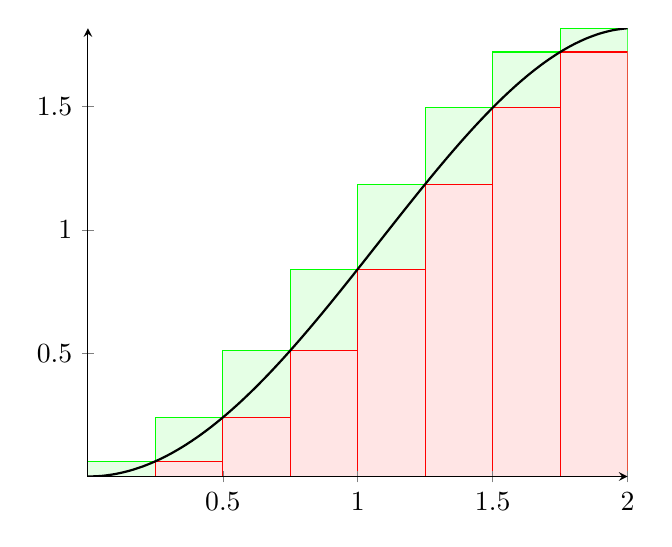
\begin{tikzpicture}[scale=1.0]
\begin{axis}[
    % xtick={0,...,1.5},ytick={0,...,1.5},
    % xmax=2,ymax=1.2,ymin=0,xmin=0,
    % enlargelimits=true,
    axis lines=middle,
    % clip=false,
    domain=0:2,
    axis on top
    ]

\addplot [draw=green, fill=green!10, const plot mark right, samples=9, domain=0:2]
    {x * sin(deg(x))}\closedcycle;
\addplot [draw=red, fill=red!10, ybar interval, samples=9, domain=0:2]
    {x * sin(deg(x))}\closedcycle;

\addplot[smooth, thick,domain=0:2,samples=40]{x * sin(deg(x))};
\end{axis}
\end{tikzpicture}
\caption{Somme di Riemann inferiori e superiori}
\end{figure}

Suddividiamo in un certo numero di rettangoli il sottografico della funzione. Disegnamo $n$ rettangoli, ciascuno con un area (data dalla base per l'altezza), e la somma delle aree \`e minore dell'area che vogliamo calcolare.

I punti scelti costituiscono una partizione dell'intervallo $[a,b]$. Se prendiamo una partizione pi\`u fitta, ottenendo quindi pi\`u rettangoli, la somma delle aree dei rettangoli \`e maggiore a quella precedente, ed \`e pi\`u vicina all'area che vogliamo calcolare.

Questa \`e l'idea di tal Cavalieri, il ``principio di esaustione''. Infittendo la partizione si approssima sempre meglio l'area sotto la curva.

Si pu\`o calcolare la somma delle aree dei rettangoli costruibili \emph{sopra} al grafico. L'area della somma di questi rettangoli \emph{contiene} l'area della funzione. In questo caso, infittendo la partizione, l'area diminuisce.

Vogliamo che queste due aree, quella sopra e quella sotto al grafico, siano, al limite, uguali. Se esiste un punto a cui queste due somme tendono, quel punto sar\`a proprio l'integrale.

\subsection{Somme di Riemann}

Consideriamo ora una funzione $f(x)$, e una partizione $P = \{ x_1, x_2, \ldots, x_n \}$ con $a = x_1 < x_2 < \ldots < x_{n-1} < x_n = b$.

Ora, per ogni coppia $[x_{i-1}, x_{i}]$ prendiamo due punti $l_i, u_i \in [x_{i-1}, x_{i}]$, tali che $f(l_i) \le f(x) \le f(u_i) \forall x \in [x_{i-1},x_{i}]$. I due punti $l_i$ e $u_i$ sono i punti di massimo e minimo della funzione nell'$i$-esimo intervallo.

Stiamo facendo l'ipotesi che in ciascuno di questi intervalli la funzione sia dotata di massimo e di minimo. Il teorema di Weierstrass ce lo garantisce, se la funzione \`e continua nell'intervallo.

Tenendo conto di queste notazioni, chiamiamo $L(P,f)$ la somma delle aree ``sotto'' la funzione, ossia:
\[
L(P,f) = \sum_{i = 1}^{n} f(l_i) \cdot (x_{i} - x_{i-1})
\]
Allo stesso modo, definiamo la somma $U(P,f)$ delle aree sopra la funzione:
\[
U(P,f) = \sum_{i = 1}^{n} f(u_i) \cdot (x_{i} - x_{i-1})
\]
\`E evidente che $L(P,f) \le U(P,f)$. Queste due quantit\`a si chiamano somme di Riemann, somma inferiore la prima e somma superiore la seconda.

Consideriamo due partizioni differenti, $P'$ e $P''$, vale sempre che $L(P',f) \le U(P'',f)$, anche se gli intervalli su cui ciascuna somma \`e basata sono differenti. Una somma fatta dal basso \`e sempre minore o uguale di una somma fatta dall'altro anche con una partizione differente.

Ora possiamo definire l'integrale definito, o integrale di Riemann.

\begin{defn}[Integrale di Riemann]
Se esiste un unico numero $I$ tale che $L(P',f) \le I \le U(P'',f) \forall P', P''$, allora $I$ sar\`a l'integrale di Riemann da $a$ a $b$:
\[
I = \int_{a}^{b} f(x) \dx
\]
\end{defn}
Questo \`e anche l'integrale definito, ma guai (per ora!) pensare di aver gi\`a visto il simbolo di integrale. \`E un simbolo con significato \emph{diverso} dal simbolo di integrale indefinito.

Come pu\`o succedere che non esista un unico numero $I$ che rispetta queste condizioni?

Consideriamo la funzione di Dirichlet, definita come segue:
\[
f(x) = 
\begin{cases}
1 \text{ se } x \in [0,1] \cap \rationals \\
0 \text{ se } x \notin [0,1] \setminus \rationals
\end{cases}
\]
Questa funzione non si pu\`o disegnare. Facciamo le somme di Riemann superiori e inferiori. In ogni intervallo abbiamo sia numeri razionali che numeri irrazionali. Il valore minimo della funzione \`e sempre 0, e il valore massimo \`e sempre 1, qualunque intervallo si scelga. Fra la somma inferiore e la somma superiore ci sono infiniti numeri, e non si pu\`o attribuire un'area al sottografico di questa funzione.

Se la funzione $f$ di cui vogliamo trovare l'area non \`e una funzione positiva nell'intervallo $[a,b]$ in cui cerchiamo l'area, che senso ha quello che stiamo facendo? Dobbiamo iniziare a parlare di \emph{area con segno}: consideriamo negativa un'area sotto l'asse delle $x$. I rettangoli che compongono la somma inferiore saranno pi\`u grandi dei rettangoli della somma superiore, ma attribuendogli un valore negativo la loro area resta minore dell'area dei rettangoli della somma superiore.

\begin{theorem}
\label{integrale_funzione_continua}
Se $f \in C^{0}([a,b])$ ($f$ \`e continua in $[a,b]$), allora esiste l'integrale definito $\int_{a}^{b} f(x) \dx$.
\end{theorem}

\begin{theorem}
Se $f \in C^{1}([a,b])$, ossia se $f$ \`e derivabile e $f'$ \`e continua in $[a,b]$, allora esiste l'integrale definito $\int_{a}^{b} f(x) \dx$.
\end{theorem}
Dimostrarlo per esercizio.

La scrittura $f \in C^{n} ([a,b])$ indica che la funzione $f$ \`e continua, \`e derivabile $n$ volte nell'intervallo $[a,b]$, e ognuna delle $n$ derivate \`e continua in $[a,b]$.

\begin{theorem} \label{integrabilita_riemann}
Usando le somme di Riemann si pu\`o stabilire se esiste l'integrale di Riemann.
\[
\exists \int_{a}^{b} f(x) \dx \iff \forall \epsilon > 0 \exists P \text{ t.c. } U(P,f) - L(P,f) < \epsilon
\]
Ossia, una funzione ha integrale di Riemann se e solo se la differenza fra le due somme (superiore e inferiore) pu\`o essere resa arbitrariamente piccola (con un'opportuna partizione).
\end{theorem}

\begin{oss}
Data una partizione $P$ di $[a,b]$, sia $c_i \in [x_{i-1},x_i]$ un punto qualunque nell'$i$-esimo intervallo determinato dalla partizione. Osserviamo che $f(l_i) \le f(c_i) \le f(l_i)$. Possiamo quindi scrivere che:
\[
L(P,f) = \sum_{i = 1}^{n} f(l_i) \cdot (x_{i} - x_{i - 1}) \le \sum_{i = 1}^{n} f(c_i) \cdot (x_{i} - x_{i - 1}) \le \sum_{i = 1}^{n} f(u_i) \cdot (x_{i} - x_{i - 1}) = U(P,f)
\]
\`E chiaro che se la funzione \`e integrabile, la somma di mezzo viene \emph{schiacciata} dalle altre due.
\end{oss}

Con questa osservazione possiamo tirare fuori una versione diversa del teorema \ref{integrabilita_riemann}.
\[
\int_{a}^{b} f(x) \dx = \lim_{\norm{P} \to 0} \sum_{i = 1}^{n} f(c_i) \cdot (x_i - x_{i - 1})
\]
La norma di $P$ ($\norm{P}$) \`e la massima lunghezza di un intervallo, ossia $\norm{P} = \max(x_i - x_{i-1})$.

% L'area del sottografico \`e l'area compresa fra il grafico e l'asse delle $x$. Se l'asse $x$ \`e sopra il grafico, l'area per convenzione ha segno negativo.

% L'integrale di una funzione dispari su un intervallo simmetrico rispetto all'asse $y$ \`e sempre nullo.

\subsection{Considerazioni sugli integrali definiti}

Per definizione, con gli integrali definiti vale:
\[
\int_{b}^{a} f(x) \dx = - \int_{a}^{b} f(x) \dx
\]
Facciamo qualche considerazione pi\`u o meno banale.
\begin{enumerate}
    \item Se $f(x) \le g(x)$ in $[a,b]$, allora:
    \[
    \int_{a}^{b} f(x) \dx \le \int_{a}^{b} g(x) \dx
    \]
    \item L'integrale definito \`e lineare:
    \[
    \int_{a}^{b} \left[ A \, f(x) + B \, g(x) \right] \dx =
    A \int_{a}^{b} f(x) \dx + B \int_{a}^{b} g(x) \dx
    \]
    Vederlo in maniera geometrica non \`e immediato. Ma abbiamo visto che le derivate sono lineari, visto che le derivate sono limiti e i limiti a loro volta sono lineari. Scriviamo questo integrale come limite, considerando una partizione $P = \{ x_1, x_2, \ldots, x_n \}$ e i punti $c_i \in [x_{i-1}, x_{i}]$:
    \[
    \lim_{\norm{P} \to 0} \sum_{i = 1}^{n} \left[ A \, f(c_i) + B \, g(c_i) \right] \cdot (x_{i} - x_{i-1})
    \]
    Ma il limite della combinazione lineare, abbiamo detto, \`e la combinazione lineare dei limiti:
    \[
    A \, \lim_{\norm{P} \to 0} \sum_{i = 1}^{n} f(c_i) \cdot (x_{i} - x_{i - 1}) +
    B \, \lim_{\norm{P} \to 0} \sum_{i = 1}^{n} g(c_i) \cdot (x_{i} - x_{i - 1})
    \]
    Questa quantit\`a \`e esattamente $A$ volte l'integrale definito di $f(x)$ pi\`u $B$ volte l'integrale definito di $g(x)$.
    \item Se $a < c < b$ ed esiste l'integrale definito $\int_{a}^{b} f(x) \dx$, allora:
    \[
    \int_{a}^{b} f(x) \dx = \int_{a}^{c} f(x) \dx + \int_{c}^{b} f(x) \dx
    \]
    \item Vale questa propriet\`a:
    \[
    \abs{\int_{a}^{b} f(x) \dx} \le \int_{a}^{b} \abs{f(x) \dx}
    \]
    \`E simile alla tipica disuguaglianza triangolare: $\abs{a + b} \le \abs{a} + \abs{b}$.
    \item Considerando integrali definiti su intervalli simmetrici rispetto all'asse $y$, se $f$ \`e pari vale che:
    \[
    \int_{-b}^{b} f(x) \dx = 2 \, \int_{0}^{b} f(x) \dx
    \]
    Se \`e dispari, vale invece che:
    \[
    \int_{-b}^{b} f(x) \dx = 0
    \]
\end{enumerate}

\subsubsection{Teorema del valor medio applicato agli integrali definiti}

Consideriamo un integrale definito di una funzione continua:
\[
\int_{a}^{b} f(x) \dx
\]
Siano, per il teorema di Weierstrass, $m = \min_{[a,b]} f(x)$ e $M = \max_{[a,b]} f(x)$. Possiamo minorare e maggiorare l'integrale definito come segue:
\[
\int_{a}^{b} m \dx \le \int_{a}^{b} f(x) \dx \le \int_{a}^{b} M \dx
\]
Si vede facilmente che $\int_{a}^{b} M \dx = M \cdot (b - a)$, e quindi che:
\[
m \cdot (b - a) \le \int_{a}^{b} f(x) \dx \le M \cdot (b - a) \implies
m \le \frac{1}{b - a} \int _{a}^{b} f(x) \dx \le M
\]
La funzione \`e continua per ipotesi, quindi assume tutti i valori fra minimo e massimo. Questo vuol dire che $\exists c \in (a,b)$ tale per cui:
\[
\frac{1}{b - a} \int_{a}^{b} f(x) \dx = f(c)
\]
Geometricamente, vuol dire che l'area sotto la funzione \`e uguale all'area del rettangolo alto $f(c)$ e largo quanto l'intervallo preso in esame, anche se non conosciamo dove sia il punto $c$.

\begin{exmp}
Consideriamo l'integrale definito $\int_{0}^{2} x \dx$, e la partizione $P_n$ dell'intervallo $[0,2]$ in sottointervalli ciascuno di lunghezza $\frac{2}{n}$. La differenza fra le somme inferiori e superiori di Riemann \`e:
\[
U(P_n, f) - L(P_n, f) = \sum_{i = 1}^{n} \left[ f(u_i) - f(l_i) \right] \cdot \frac{2}{n} = n \cdot \frac{4}{n^2}
\]
L'integrale definito di questa funzione, in questo intervallo, esiste: $\forall \epsilon > 0, \exists N_{\epsilon}$ tale per cui la differenza sopra \`e minore di $\epsilon$, per ogni $n \ge N_{\epsilon}$. Infatti basta che valga:
\[
n > \frac{4}{\epsilon}
\]
Si pu\`o poi far vedere quanto vale questo integrale definito, trovando i limiti delle somme inferiori o delle somme superiori.
\[
\int_{0}^{2} x \dx = 2 = \lim_{n \to \infty} U(P_n, f) = \lim_{n \to \infty} L(P_n, f)
\]
Infatti:
\[
\lim_{n \to \infty} U(P_n,f) = 
\lim_{n \to \infty} \sum_{i = 1}^{n} \frac{i \, 2}{n} \cdot \frac{2}{n} = \lim_{n \to \infty} \frac{4}{n^2} \cdot \sum_{i = 1}^{n} i =
\lim_{n \to \infty} \frac{\cancelto{2}{4}}{\cancel{n^2}} \cdot \frac{\cancel{n^2} + \cancelto{0}{n}}{\cancel{2}} = 2
\]
\end{exmp}

Salvo in casi particolari, l'unico modo per calcolare integrali definiti \`e attraverso l'approssimazione.

\section{Teorema fondamentale del calcolo}

Il teorema fondamentale del calcolo vale per ogni $f \in C^{0} ([a,b])$ (ossia per ogni funzione continua nell'intervallo chiuso e limitato $[a,b]$).

\begin{theorem}[Teorema fondamentale del Calcolo]
Sia $F(x) = \int_{a}^{x} f(t) \dx[t]$, per $a \le x \le b$, ossia la funzione che calcola l'area sotto il grafico della funzione $f$ dal punto $a$ al punto (variabile) $x$, allora:
\begin{enumerate}
    \item $\exists F'(x) = f(x)$
    \item $\forall G$ primitiva di $f$ in $[a,b]$, risulta che:
    \[
    \int_{a}^{b} f(x) \dx = G(b) - G(a) = \increment{\int f(x) \dx}_{a}^{b}
    \]
    L'ultima parte si legge ``incremento dell'integrale indefinito da $a$ a $b$''.
\end{enumerate}
\end{theorem}
Nella premessa, $x$ indica l'estremo superiore di integrazione, mentre la $t$ \`e una variabile muta di integrazione (e quindi non \`e minimamente rilevante la lettera che gli si associa).

La nozione di primitiva di una funzione e quella di area individuata dal grafo della funzione sono legate a doppio filo dal teorema fondamentale del Calcolo.

\begin{proof}
Calcoliamo la derivata della funzione $F(x)$.
\begin{align*}
\lim_{h \to 0} \frac{F(x + h) - F(x)}{h} = 
\lim_{h \to 0} \frac{1}{h} \, \left[ \int_{a}^{x+h} f(t) \dx[t] - \int_{a}^{x} f(t) \dx[t] \right] = \tag{per additivit\`a degli integrali} \\
= \lim_{h \to 0} \frac{1}{h} \, \left[ \cancel{\int_{a}^{x} f(t) \dx[t]} + \int_{x}^{x+h} f(t) \dx[t] - \cancel{\int_{a}^{x} f(t) \dx[t]} \right]
= \lim_{h \to 0} \frac{1}{h} \, \int_{x}^{x+h} f(t) \dx[t] = \tag{per il valor medio} \\
= \lim_{h \to 0} \frac{1}{h} \cdot f(c) \cdot (\cancel{x} + h - \cancel{x}) = \lim_{h \to 0} f(c) \cdot \frac{\cancel{h}}{\cancel{h}} = \lim_{h \to 0} f(c)
\end{align*}
Con $c \in [x, x+h]$, ma per $h \to 0$, si ha che $c \to x$, e quindi la derivata di $F(x)$ (che \`e la funzione che calcola l'area sotto $f(x)$) \`e proprio $f(x)$. 

Vediamo poi che se $G'(x) = f(x)$, allora $G(x) + c = \int_{a}^{x} f(t) \dx[t]$. Cosa segue da questo?

Prima di tutto, prendendo $x = a$, si ha che $G(a) + c = 0$, e quindi $c = - G(a)$.

Poi, prendendo $x = b$, abbiamo che $\int_{a}^{b} f(t) \dx[t] = G(b) + c = G(b) - G(a)$. E quindi una qualsiasi primitiva di $f(x)$ \`e la funzione che calcola l'area sotto il grafico di $f(x)$!
\end{proof}

\subsection{Integrali definiti e derivate}
\label{derivate_di_integrali}

Abbiamo detto che se $f \in C^0 ([a,b])$, ossia se \`e continua in $[a,b]$, allora $f$ \`e integrabile in $[a,b]$, e in particolare per ogni punto $x \in [a,b]$:
\[
F(x) = \int_{a}^{x} f(x) \dx
\]
Facendo variare il punto $x$ si ottiene una funzione che dipende da $x$. Il teorema fondamentale del calcolo integrale ci dice che questa funzione $F(x)$ \`e derivabile, e la derivata \`e la funzione integranda $f(x)$.

Cosa vuol dire questo?
\[
G(x) = \int_{a}^{x^2} f(t) \dx[t]
\]
Vuol dire che $G(x) = F(x^2)$. Infatti, se sostituiamo nell'equazione che segue $y$ con $x^2$, otteniamo la stessa cosa.
\[
F(y) = \int_{a}^{y} f(t) \dx[t]
\]
Se deriviamo $G(x)$ cosa succede?
\[
\deriv{x} G(x) = \deriv{x} F(x^2) = 2 \, x \, f(x^2)
\]
Basta applicare la regola di derivazione delle funzioni composte.

Una nota pedante sulla derivata delle funzioni composte. La derivata di una funzione, come $F(x^2)$, si scrive come la derivata della funzione ``esterna'' $F$ \emph{calcolata} in $x^2$ per la derivata della funzione ``interna'', $x^2$. Si scrive cos\`i:
\[
\deriv{x} F(x^2) = \left( \deriv{y} F \right) \left( x^2 \right) \cdot \deriv{x} \left( x^2 \right)
\]

\begin{exmp}
Guardiamo questa funzione:
\[
G(x) = \int_{0}^{\sin(x)} \frac{1}{1 + t^2} \dx[t]
\]
La sua derivata $G'(x)$ \`e:
\[
G'(x) = \frac{\cos(x)}{1 + \sin^2(x)} = \frac{\cancel{\cos(x)}}{\cos^{\cancel{2}}(x)} = \frac{1}{\cos(x)}
\]

Guardiamo questa:
\[
G(x) = \int_{a}^{\tan \left[ \log(1 + x^2) \right]} \arctan \left[ e^{t^2 + \cos(t)} \right] \dx[t]
\]
Non possiamo neanche lontanamente pensare di trovare l'integrale di questo mostro. Noi vogliamo solo calcolare $G'(x)$. Si prende la funzione integranda e la si calcola nell'estremo superiore, e la si moltiplica per la derivata dell'estremo superiore.
\begin{align*}
G'(x) &= \arctan \left[ e^{{\tan \left[ \log(1 + x^2) \right]}^2 + \cos \left( \tan \left[ \log(1 + x^2) \right] \right)} \right] \cdot \left[ \tan \left[ \log(1 + x^2) \right] \right]' = \\
&= \arctan \left[ e^{{\tan \left[ \log(1 + x^2) \right]}^2 + \cos \left( \tan \left[ \log(1 + x^2) \right] \right)} \right] \cdot \frac{1}{\cos^2 \left[ \log(1 + x^2) \right]} \cdot \frac{1}{1 + x^2} \cdot 2 \, x
\end{align*}

Questi esempi infami servono a capire cosa significa il teorema fondamentale del calcolo, ossia che l'integrale $\int_{a}^{x} f(t) \dx[t] = F(x)$ \`e tale che $F'(x) = f(x)$. Quindi la derivata di questo integrale \`e immediata:
\[
\deriv{x} \int_{a}^{x} \cos (\tan(1 + t^2)) \cdot e^{\arctan(\log(1+t^{2 \, \cos^2(t)}))} \dx[t] = 
\cos (\tan(1 + x^2)) \cdot e^{\arctan(\log(1+x^{2 \, \cos^2(x)}))}
\]
Per calcolare la derivata della funzione $F(x)$ non dobbiamo conosccere la funzione $F(x)$, perch\'e conosciamo la funzione $f(x)$.

E se volessimo derivare un integrale che ha delle funzioni in entrambi gli estremi di integrazione?
\[
G(x) = \int_{\tan(x^2)}^{e^{2x + \cos^2(x)}} \left[ t^a + \log(1 + t^2) \right] \dx[t]
\]
A esser precisi bisognerebbe dire che la $x$ \`e compresa fra $- \frac{\pi}{2}$ e $\frac{\pi}{2}$. Comunque, sappiamo come spezzare questo integrale:
\[
G(x) = \int_{0}^{e^{2x + \cos^2(x)}} \left[ t^a + \log(1 + t^2) \right] \dx[t] - \int_{0}^{\tan(x^2)} \left[ t^a + \log(1 + t^2) \right] \dx[t]
\]
Si possono scambiare gli estremi di integrazione invertendo il segno dell'integrale. Adesso sapppiamo come calcolare la derivata di $G(x)$.
\begin{align*}
G'(x) =& e^{2a \, x + a \, \cos^2(x)} + \log(1 + e^{4 \, x + 2 \, \cos^2(x)}) \cdot e^{2 \, x + \cos^2 (x)} \cdot \left( 2 - 2 \, \sin(x) \cos(x) \right) + \\
&-  {\tan(x^2)}^a + \log(1 + {\tan(x^2)}^2) \cdot \frac{1}{\cos^2(x)} \cdot 2 \, x
\end{align*}

In questo caso non abbiamo assolutamente modo di trovare la primitiva di $f(x)$:
\[
G(x) = \int_{\sin(x)}^{\cos^2(x)} e^{-t^2} \dx[t]
\]
Ma sappiamo sempre trovare la derivata di $G(x)$.
\[
G'(x) = e^{-{\left[ \cos^2(x) \right]}^2} \cdot (- 2 \sin(x) \cos(x)) - 
e^{-\sin^2(x)} \cdot \cos(x)
\]
\end{exmp}

Se adesso vogliamo tirare fuori un caso generale, possiamo scrivere che, dato questo integrale:
\[
G(x) = \int_{\alpha (x)}^{\beta (x)} f(t) \dx[t]
\]
la sua derivata \`e:
\[
G'(x) = f(\beta(x)) \cdot \beta'(x) - f(\alpha(x)) \cdot \alpha'(x)
\]
per il teorema fondamentale del calcolo.

\subsection{Funzioni continue a tratti}

Un esempio di funzione continua a tratti \`e la funzione parte intera.
\[
f(x) = \left[ x \right]
\]
Supponiamo ora di voler calcolare l'integrale:
\[
\int_{\frac{3}{2}}^{4} \left[ x \right] \dx
\]
\begin{figure}[h]
\centering
\begin{tikzpicture}
    \begin{axis}[
            xmin=0,xmax=5,
            ymin=0,ymax=5,
            axis x line=middle,
            axis y line=left,
            axis line style={->},
            % xlabel={$\reals$},
        ]
        \addplot[line width=2pt,-,domain=0:1]{0};
        \addplot[line width=2pt,-,domain=1:2]{1};
        \addplot[line width=2pt,-,domain=2:3]{2};
        \addplot[line width=2pt,-,domain=3:4]{3};
        \addplot[line width=2pt,-,domain=4:5]{4};
        \addplot[fill=black,only marks,mark=*]coordinates{(0,0)(1,1)(2,2)(3,3)(4,4)};
    \end{axis}
\end{tikzpicture}
\caption{La funzione ``parte intera''}
\end{figure}

La funzione non \`e continua, e non \`e continua neanche nell'intervallo [1,2]. \`E continua solo nell'intervallo [1,2) che ha un estremo non chiuso! Ma l'area sotto il rettangolo [1,2] \`e identica all'area sotto il rettangolo [1,2), poich\'e differiscono di un solo segmento.

Quindi l'integrale che abbiamo visto vale:
\[
\int_{\frac{3}{2}}^{4} \left[ x \right] \dx =
\int_{\frac{3}{2}}^{2} \left[ x \right] \dx +
\int_{2}^{3} \left[ x \right] \dx +
\int_{3}^{4} \left[ x \right] \dx
\]

\section{Integrali impropri}

Sappiamo calcolare l'integrale indefinito di:
\[
\int \log (x) \dx = x \, \log (x) - x + c
\]
Poi, $\forall a \ge 0$, sappiamo calcolare questo integrale definito:
\[
\int_{a}^{1} \log (x) \dx = - 1 - a \, \log (a) + a
\]
Facendo il limite per a che tende a $0^+$, vediamo che quest'area vale:
\[
\lim_{a \to 0^+} \int_{a}^{1} \log (x) \dx = -1
\]
Sappiamo calcolare qualunque area di questo tipo, $\forall a, b \ge 0$:
\[
\int_{a}^{b} \log (x) \dx
\]
Abbiamo parlato solo di intervalli $[a,b]$ chiusi e limitati. La cosa pi\`u estrema che abbiamo fatto \`e stato togliere un punto dall'estremo dell'intervallo. Ma in questo caso, se studiamo $\log (x)$ nell'intervallo $(0,1]$, la funzione \`e continua \emph{ma non} limitata.

Prendendo per\`o un qualunque $a \in (0,1]$, la funzione nel punto $a$ \`e sia continua che limitata. Facendo tendere $a$ a $0^+$ vediamo che l'area sotto la funzione \`e limitata, e tende a $-1$. La cosa rilevante \`e che abbiamo attribuito un'area limitata al grafico di una funzione su un insieme illimitato. Adesso possiamo ammettere questo:
\[
\int_{0}^{1} \log (x) \dx = -1
\]
Questo \`e un integrale improprio. Un integrale improprio \`e il limite di un integrale proprio.

\begin{exmp}
Quello che segue \`e un normale integrale definito, per $b \in \reals$.
\[
\int_{1}^{b} \frac{\diff x}{1 + x^2} = \arctan (b) - \frac{\pi}{4}
\]
Ma se facciamo il limite per $b \to \infty$, l'integrale diventa un integrale improprio.
\[
\lim_{b \to \infty} \int_{1}^{b} \frac{\diff x}{1 + x^2} = \frac{\pi}{2} - \frac{\pi}{4} = \frac{\pi}{4}
\]
\end{exmp}

\begin{exmp}
Questo \`e immediatamente riconoscibile come un integrale improprio:
\[
\int_{0}^{1} \frac{\diff x}{x}
\]
La funzione integranda, infatti, non \`e definita in uno degli estremi di integrazione (nello specifico, in 0). Quindi trovare un integrale simile vuol dire trovare questo integrale:
\[
\lim_{a \to 0^+} \int_{a}^{1} \frac{\diff x}{x} =
\lim_{a \to 0^+} \log(1) - \log(a) = 
- \lim_{a \to 0^+} \log(a) = \infty
\]
Qui abbiamo quindi una funzione illimitata su un intervallo limitato, e il suo integrale non esiste.
\end{exmp}

\begin{exmp}
Variazioni sullo stesso integrale improprio.
\[
\int_{1}^{\infty} \frac{\diff x}{x}
\]
Anche questo \`e improprio. Abbiamo una funzione integranda che (in $[1, \infty)$) \`e limitata, nonostante l'intervallo preso non lo sia.
\[
\lim_{b \to \infty} \int_{1}^{b} \frac{\diff x}{x} = \lim_{b \to \infty} \log(b) = \infty
\]
\end{exmp}

Quindi l'integrale definito di $\frac{1}{x}$ non esiste n\'e fra 0 e 1, n\'e fra 1 e $\infty$. $\frac{1}{x}$ \`e una funzione illimitata in 0 e all'infinito. Sar\`a sempre cos\`i, con tutte le funzioni non limitate?

\begin{exmp}
L'integrale che segue sembra simile ai casi precedenti, ma... 
\[
\int \frac{\diff x}{x^2} = - \frac{1}{x} + c
\]
Rifacciamo entrambi i ``test'' fatti prima.
\begin{align*}
\int_{0}^{1} \frac{\diff x}{x^2} \\
\int_{1}^{\infty} \frac{\diff x}{x^2}
\end{align*}
Sempre due integrali impropri. Ma vogliamo capire quale integrale converge e quale diverge.
\[
\lim_{a \to 0^+} \int_{a}^{1} \frac{\diff x}{x^2} =
\lim_{a \to 0^+} - 1 + \frac{1}{a} = \infty
\]
Diverge fra 0 e 1...
\[
\lim_{b \to \infty} \int_{1}^{b} \frac{\diff x}{x^2} =
\lim_{b \to 0^+} - \frac{1}{b} + 1 = 1
\]
E converge a 1 fra 1 e $\infty$.
\end{exmp}

\begin{exmp}
Vediamo un altro caso apparentemente simile ai precedenti. 
\[
\int \frac{\diff x}{\sqrt{x}} = 2 \, \sqrt{x} + c
\]
Quale integrale improprio converge, e quale diverge?
\[
\lim_{a \to 0^+} \int_{a}^{1} \frac{\diff x}{\sqrt{x}} =
\lim_{a \to 0^+} 2 - 2 \, \sqrt{a} = 2
\]
Converge (a 2) fra 0 e 1...
\[
\lim_{b \to \infty} \int_{1}^{b} \frac{\diff x}{\sqrt{x}} =
\lim_{b \to 0^+} 2 \, \sqrt{b} - 2 = \infty
\]
E diverge fra 1 e $\infty$.
\end{exmp}

\subsection{Funzioni razionali e integrali impropri}
\label{integrali_impropri_razionali}

Conosciamo l'integrale di questa funzione generica:
\[
\int \frac{\diff x}{x^p} = 
\begin{cases}
\dfrac{x^{-p + 1}}{- p + 1} + c & \text{ se } p \neq 1 \\
\abslog{x} + c & \text{ se } p = 1
\end{cases}
\]
Vogliamo studiare due integrali impropri a partire da questa funzione generica.
\begin{align*}
\int_{0}^{1} \frac{\diff x}{x^p} \qquad
\int_{1}^{\infty} \frac{\diff x}{x^p}
\end{align*}
\`E chiaro che, per $p$ negativo o nullo ($p \le 0$), il primo \`e un integrale proprio (la funzione, infatti, \`e continua e limitata anche in 0). I casi interessanti sono quelli per $p > 0$. Vogliamo capire per quali valori di $p$ questo integrale converge e per quali diverge.

Abbiamo visto che se $p = \frac{1}{2}$ il primo converge, il secondo diverge, mentre se $p = 2$ il primo diverge e il secondo converge.

Vediamo il primo integrale improprio nel caso generico, per $p \neq 1$:
\[
\int_{0}^{1} \frac{\diff x}{x^p} = 
\lim_{a \to 0^+} \int_{a}^{1} \frac{\diff x}{x^p} =
\lim_{a \to 0^+} \frac{1}{- p + 1} - \frac{a^{-p + 1}}{-p + 1}
\]
Ora, tutto dipende da $-p + 1$. Per a che tende a $0^+$, $a^n$ tende a $0$ se l'esponente \`e positivo, o a $\infty$ se l'esponente \`e negativo. Quindi:
\[
\lim_{a \to 0^+} \frac{1}{- p + 1} - \frac{a^{-p + 1}}{-p + 1} =
\begin{cases}
\dfrac{1}{- p + 1} & \text{ se } p < 1 \\
\infty & \text{ se } p > 1
\end{cases}
\]
Se $p < 1$, abbiamo che $-p > - 1 \implies - p + 1 > 0$.

Vediamo l'altro integrale.
\[
\int_{1}^{\infty} \frac{\diff x}{x^p} =
\lim_{b \to \infty} \int_{1}^{b} \frac{\diff x}{x^p} = 
\begin{cases}
\text{qualcosa} \in \reals & \text{ se } p > 1 \\
\infty & \text{ se } p \le 1
\end{cases}
\]

\subsubsection{Recap}

Nell'intervallo $\ocint{0}{1}$ vale questo:
\[
\int_{0}^{1} \frac{\diff x}{x^p} = 
\begin{cases}
\dfrac{1}{- p + 1} & \text{ se } p < 1 \\
\infty & \text{ se } p \ge 1
\end{cases}
\]
Nell'intervallo $\coint{1}{\infty}$ vale questo:
\[
\int_{1}^{\infty} \frac{\diff x}{x^p} =
\begin{cases}
\text{qualcosa} \in \reals & \text{ se } p > 1 \\
\infty & \text{ se } p \le 1
\end{cases}
\]
E basta.

\begin{exmp}
Basta integrali impropri di funzioni razionali.
\[
\int_{0}^{\infty} x \, e^{-x} \dx =
\lim_{b \to \infty} \int_{0}^{b} x \, e^{-x} \dx = 
\increment{\lim_{b \to \infty} -x \, e^{-x} - e^{-x}}_{0}^{b} =
\lim_{b \to \infty} -b \, e^{-b} - e^{-b} + 1 = + 1
\]
\end{exmp}

\begin{exmp}
Studiamo questo integrale improprio:
\[
\int_{- \infty}^{\infty} e^{-\abs{x}} \dx
\]
La funzione \`e pari, ed \`e limitata. La scriviamo come somma di due integrali impropri:
\begin{align*}
\int_{0}^{\infty} e^{-x} \dx + \int_{-\infty}^{0} e^{x} \dx =
2 \, \int_{0}^{\infty} e^{-x} \dx &= \\
2 \, \lim_{b \to \infty} \int_{0}^{b} e^{-x} \dx = 
\increment{2 \, \lim_{b \to \infty} - e^{-x}}_{0}^{b} = 
2 \, \lim_{b \to \infty} - e^{-b} + e^{0} &= 2
\end{align*}
\end{exmp}

\subsection{Criterio del confronto per determinare la convergenza}

Non tutti gli integrali sono simpatici, non di tutti gli integrali sappiamo trovare l'integrale indefinito.
\[
\int_{0}^{\infty} e^{-x^2} \dx
\]
Non serve a molto riscriverlo cos\`i:
\[
\lim_{b \to \infty} \int_{0}^{b} e^{-x^2} \dx
\]
perch\'e non sappiamo trovare l'integrale indefinito! Ma possiamo usare un criterio del confronto, dicendo prima questo:
\[
e^{-x^2} \le e^{-x}
\]
e quindi:
\[
\lim_{b \to \infty} \int_{0}^{b} e^{-x^2} \dx \le
\lim_{b \to \infty} \int_{0}^{b} e^{-x} \dx = 1
\]

Sono sempre e solo due le cose che si possono fare, per vedere se un integrale improprio converge o diverge:
\begin{enumerate}
    \item maggiorare l'integrale dato con un integrale che converge, e scoprire quindi che l'integrale dato converge, oppure
    \item minorare l'integrale dato con un integrale che diverge, e scoprire quindi che l'integrale dato diverge.
\end{enumerate}

\begin{exmp}
Scopriamo se questo integrale (improprio) converge o diverge.
\[
\int_{-1}^{0} \frac{e^x}{x+1} \dx
\]
\`E improprio, perch\'e per $x$ che tende a $-1$ la funzione integranda tende all'infinito. In 0 la funzione \`e definita (e vale 1).

Si pu\`o vedere che vale questa disuguaglianza, sapendo che $e^0$ vale 1:
\[
\frac{e^x}{x+1} \le \frac{1}{x+1} \text{ per } x \in \ocint{-1}{0}
\]
Infatti sappiamo che $e^x$ in $\ocint{-\infty}{0}$ \`e crescente, con massimo in $0$, e il massimo vale 1. Quindi $e^x$ in $\ocint{-\infty}{0}$ si maggiora con 1!

Per\`o \`e una maggiorazione inutile, visto che la funzione con cui abbiamo maggiorato la funzione integranda \emph{non ha} un integrale convergente.

Ma in $\ccint{-1}{0}$ la funzione $e^x$ ha il minimo in $-1$, e quel minimo \`e $e^{-1}$. Quindi la funzione integranda possiamo minorarla cos\`i:
\[
\frac{e^{-1}}{x+1} \le \frac{e^x}{x+1} \text{ per } x \in \ocint{-1}{0}
\]
La funzione con cui abbiamo minorato \`e simile alla funzione con cui abbiamo maggiorato prima (\`e la funzione di prima moltiplicata per la costante $e^{-1}$), quindi anche l'integrale di questa funzione diverge. Avendo minorato, in questo caso, abbiamo capito che l'integrale improprio iniziale \emph{diverge}.
\end{exmp}

C'\`e una certa disuguaglianza molto importante:
\[
0 \le \frac{\sin(x)}{x} \le 1
\]

\begin{exmp}
La disuguaglianza serve per determinare la convergenza di questo integrale:
\[
\int_{0}^{\frac{\pi}{2}} \frac{\sin(x)}{x^{\frac{7}{4}}} \dx
\]
Prima vediamo qualcosa di sbagliato, sapendo che vale sempre $\sin(x) \le 1$:
\[
\int_{0}^{\frac{\pi}{2}} \frac{\sin(x)}{x^{\frac{7}{4}}} \dx \le
\int_{0}^{\frac{\pi}{2}} \frac{\diff x}{x^{\frac{7}{4}}}
\]
Ma questo diverge. Non serve a niente maggiorare con qualcosa che diverge.

Invece possiamo maggiorarlo con qualcosa che converge:
\[
\int_{0}^{\frac{\pi}{2}} \frac{\sin(x)}{x^{\frac{7}{4}}} \dx =
\int_{0}^{\frac{\pi}{2}} \frac{\sin(x)}{x} \, \frac{\diff x}{x^{\frac{3}{4}}} \le
\int_{0}^{\frac{\pi}{2}} \frac{\diff x}{x^{\frac{3}{4}}}
\]
E quest'ultimo, per le regole viste nella sezione \ref{integrali_impropri_razionali}, converge.
\end{exmp}

\begin{exmp}
Questo integrale:
\[
\int_{1}^{\infty} \frac{x \, \arctan(x)^2}{x^3 + \log(x)} \dx
\]
Maggioriamo il numeratore e minoriamo il denumeratore, per maggiorare tutto l'integrale:
\[
\frac{x \, \arctan(x)^2}{x^3 + \log(x)} \le \frac{x \cdot \left( \frac{\pi}{2} \right)^2}{x^3}
\]
Questo \`e simile a un integrale del tipo $\frac{1}{x^2}$, che sappiamo convergere in $\coint{1}{\infty}$. A posto.
\end{exmp}
















\clearpage

\chapter{Equazioni differenziali}

La forma generale delle equazioni differenziali \`e:
\[
y' = f(t,y)
\]
Le soluzioni saranno tutte le funzioni $y(t)$ tali che $y'(t) = f(t, y(t)) \forall t$.

Facciamo un esempio: l'accelerazione \`e la derivata seconda dello spostamento. Quindi il secondo principio della dinamica (forza = massa per accelerazione) si pu\`o scrivere come:
\[
f(t, y, y') = F = m \cdot a = m \cdot y''
\]
indicando con $y(t)$ lo spostamento al tempo $t$. La forza \`e una funzione dell'istante, dello spostamento e della velocit\`a.

Il caso pi\`u semplice che possiamo affrontare \`e:
\[
y' = a \cdot y
\]
\`E, ad esempio, l'equazione che governa il decadimento radioattivo. E si potrebbe usare per trovare l'equazione di crescita di una popolazione, indicando con $a$ il tasso di natalit\`a meno il tasso di mortalit\`a. O almeno, questa legge \emph{dovrebbe} governare il tasso di crescita (o decrescita) di una popolazione.

Una funzione che verifica $y' = a \cdot y$, per $a = 1$, \`e $e^x$. Generalizzando, ovviamente, la funzione \`e $e^{a \cdot x}$.

Quindi, $y = C \, e^{a \cdot t}$ rappresenta le infinite soluzioni di $y' = a \cdot y$. \`E facilmente verificabile. Ma noi vogliamo una soluzione unica. L'univocit\`a della risposta dipende dal \emph{dato iniziale}. Se stiamo considerando, ad esempio, una popolazione, il numero della popolazione in un certo istante $t'$ dipende dal numero della popolazione all'istante iniziale $t_0$.

Si vede subito che la funzione, all'istante iniziale, vale $y(0) = C$.

\section{Problemi di Cauchy}

Si chiama \emph{problema di Cauchy} la combo di equazione differenziale e valore iniziale:
\[
y' = a \cdot y , \, y(0) = C
\]
La soluzione (ossia la funzione $y$) \`e univoca.

Un'equazione del genere, usata per descrivere la crescita di una popolazione, \`e chiamato \emph{modello maltusiano}.

In realt\`a, l'andamento di una popolazione \`e descritta meglio da un'equazione differenziale del tipo:
\[
y' = a \, y - b \, y^2
\]
detta \emph{equazione logistica}.

Queste sono dette equazioni differenziali del primo ordine. Equazioni differenziali del secondo ordine sono equazioni differenziali contenenti una derivata seconda, come l'equazione differenziale vista all'inizio, per il secondo principio della dinamica, o l'equazione che descrive l'andamento di una molla.

%y'' = y + \omega^2
% CONTROLLARE

\subsubsection{Equazioni differenziali banali}

Un'equazione differenziale del primo ordine molto banale \`e:
\[
y' = f(t)
\]
Non merita neanche di essere chiamata un'equazione differenziale: il problema \`e soltanto trovare le primitive di $f(t)$. Le primitive sono infinite, e questo lo sappiamo. Le soluzioni sono del tipo:
\[
y(t) = \int f(t) \dx[t] = \int_{t_0}^{t} f(s) \dx[s] + C
\]
Per rendere una ricerca di primitive un problema di Cauchy, si deve imporre una condizione del tipo $y(t_0) = y_0$ (detta \emph{condizione di Cauchyt}). Ponendo $t = t_0$, l'integrale \`e 0, e quindi deve essere $C = y_0$. 

Quindi la soluzione generale di $y' = f(t)$ (con condizione di Cauchy $y(t_0) = y_0$) \`e:
\[
y(t) = \int_{t_0}^{t} f(s) \dx[s] + y_0
\]
Fine.

Le equazioni differenziali \emph{banali} sono quelle in cui il secondo membro non dipende dall'incognita, ossia quelle, come appena visto, nella forma:
\[
y' = f(t)
\]
Le equazioni differenziali (del primo ordine) interessanti sono tutte:
\[
y' = f(y)
\]
Torniamo al caso particolare in cui $f(y) = a \, y$. Una funzione che vale identicamente 0 \`e soluzione dell'equazione. Escludiamo questo caso, e scriviamo questo (nei punti in cui $y$ \`e diversa da 0):
\[
y'(t) = a \, y(t) \implies \frac{y'(t)}{y(t)} = a
\]
Se vale questo, possiamo integrare in $\diff t$.
\[
\int_{t_0}^{t} \frac{y'(s) \dx[s]}{y(s)} = a \cdot (t - t_0)
\]
Che possiamo scrivere come:
\[
\int_{y(t_0)}^{y(t)} \frac{\diff y}{y} =
\abslog{y(t)} - \abslog{y(t_0)} =
\log \left( \frac{y(t)}{y(t_0)} \right)
\]
\`E un integrale che sappiamo (e che scriviamo come frazione, senza modulo, perch\'e siamo svegli).

Tornando all'uguaglianza di prima, scriviamo questo:
\[
\log \left( \frac{y(t)}{y(t_0)} \right) = a \, (t - t_0) \implies
\frac{y(t)}{y(t_0)} = e^{a \, (t - t_0)} \implies
y(t) = y(t_0) \, e^{a \, (t - t_0)} = y(t_0) \, e^{- a \, t_0} \, e^{a \, t}
\]
La parte dipendente da $t_0$, ossia $y(t_0) \, e^{- a \, t_0}$, l'abbiamo messa all'inizio per evidenziarla meglio.

\subsection{Equazioni a variabili separabili}

Studiamo una classe delle equazioni differenziali, quella delle equazioni differenziali a variabili separabili.

Le equazioni differenziali a variabili separabili sono le equazioni differenziali riscrivibili come:
\[
y' = a(t) \cdot b(y)
\]
Ossia, per cui riusciamo a identificare e a separare due funzioni dipendenti una dalla $y$ e una dalla $t$ (con $y = y(t)$). Queste equazioni si possono riscrivere cos\`i:
\[
\int \frac{\diff y}{b(y)} = \int a(t) \dx[t]
\]
solo negli intervalli in cui $b(y)$ \`e diversa da 0, ovviamente.
\begin{exmp}[di equazione a variabili separabili]
L'equazione che descrive l'andamento di una popolazione \`e l'equazione logistica:
\[
y' = a \, y - b \, y^2
\]
$a$ indica la differenza fra tasso di natalit\`a e tasso di mortalit\`a. $b$ indica le interazioni (negative, due a due - da cui il segno meno e il quadrato) fra membri della popolazione. Per $b = 0$, \`e l'equazione maltusiana. 

Come si proceder\`a con la risoluzione? Scriveremo questo:
\[
\frac{y'}{a \, y - b \, y^2} = 1
\]
Da cui ricaveremo questo integrale da calcolare:
\[
\int \frac{\diff y}{a \, y - b \, y^2}
\]

Prima, per\`o, si pu\`o riscrivere l'equazione logistica in questo modo (per $b$ diverso da 0):
\[
y' = k \, y \cdot \left( 1 - \frac{y}{L} \right)
\]
$L = \frac{a}{b}$ rappresenta il massimo di popolazione sostenibile, e $k = a$.

Vedendo quest'equazione come un'equazione differenziale a variabili separabili, si vede che $a(t) = k$ e $b(y) = y \cdot \left( 1 - \frac{y}{L} \right)$.

Dobbiamo calcolare questo integrale indefinito:
\begin{align*}
\int \frac{\diff y}{y \, \left( 1 - \frac{y}{L} \right)} &= \int k \dx[t] \implies \\
\int \frac{\diff y}{y} + \int \frac{\diff x}{L - y} &= k \, t + C \implies \\
\abslog{y} - \abslog{L - y} &= \abslog{\frac{y}{L - y}} = k \, t + C 
\end{align*}
Scriviamo, esponenziando entrambi i membri, questo:
\[
\abs{\frac{y}{L - y}} = e^{k \, t} \, e^C
\]
$e^C$ \`e una costante positiva (e quindi il secondo membro \`e sempre positivo). Togliamo il modulo, e prendiamo quindi al suo posto una costante $C_1$ qualsiasi (negativa o positiva):
\begin{align*}
y &= C_1 \, e^{k \, t} \cdot (L - y) \implies \\
y \cdot (1 + C_1 \, e^{k \, t}) &= C_1 \, L \, e^{k \, t} \implies \\
y(t) &= \frac{C_1 \, L \, e^{k \, t}}{1 + C_1 \, e^{k \, t}}
\end{align*}
Con un ultimo passaggio (dividendo numeratore e denominatore per $e^{k \, t})$ otteniamo questa forma della soluzione:
\[
y(t) = \frac{C_1 \, L}{e^{- k \, t} + C_1}
\]
Il valore iniziale $u = y(0)$ sar\`a:
\[
u = \frac{C_1 \, L}{1 + C_1}
\]
Per $t \to \infty$, la funzione che abbiamo trovato tende a $L$. Quindi la popolazione tende alla soglia massima.

Nota a margine: esiste anche una versione discreta dell'equazione logistica.
\[
y_{n+1} = k \, y_n \cdot \left( 1 - \frac{y_n}{L} \right)
\]
\end{exmp}

Facciamo qualche esercizio con equazioni a variabili separabili:
\[
y' = ( \sin (t) ) \cdot (1 + y^2)
\]
Come fatto sopra, la riscriviamo in questo modo e la risolviamo:
\begin{align*}
\int \frac{\diff y}{1+y^2} &= \int \sin (t) \dx[t] \implies \\
\arctan (y) &= - \cos(t) + C \implies \\
y(t) &= \tan \left( -\cos(t) + C \right)
\end{align*}
Per quali valori di $t$ \`e definita? Dipende tutto dal valore che si vuole avere all'istante iniziale. La tangente non \`e definita in $t = \frac{\pi}{2} + k \, \pi$.

Potremmo associare, ad esempio, la condizione di Cauchy che $y(0) = 0$. Dobbiamo trovare $C$:
\[
\tan \left( -1 + C \right) = 0 \implies C = \arctan ( 0 ) + 1 = 1
\]
\subsubsection{Equazioni differenziali lineari omogenee}

Considerando l'equazione differenziale generale seguente:
\[
y' = a(t) \, y
\]
La soluzione generale sar\`a:
\[
y(t) = K \, e^{A(t)}
\]
con $A'(t) = a(t)$ (ossia, $A(t)$ \`e una primitiva di $a(t)$. Equazioni differenziali di questo tipo sono dette \emph{lineari omogenee}.

\subsection{Equazioni non a variabili separabili}

Sommando a un'equazione lineare omogenea una quantit\`a dipendente solamente dalla $t$, otteniamo un'equazione non pi\`u separabile:
\begin{equation}
\label{lineare_non_omogenea}
y' = a(t) \, y + f(t)
\end{equation}
Se $f(t)$ fosse identicamente nullo, la totalit\`a delle soluzioni l'abbiamo vista poco sopra, con le equazioni differenziali lineari omogenee.

Andiamo a studiare una funzione del tipo:
\begin{equation}
\label{variazione_costante}
y(t) = v(t) \, e^{A(t)}
\end{equation}
cercando una funzione $v(t)$ (``variazione della costante'') tale per cui questa $y(t)$ sia soluzione dell'equazione differenziale \ref{lineare_non_omogenea}. Quest'equazione \`e detta \emph{lineare non omogenea}.

Allora: noi vogliamo che $y(t)$ (nell'equazione \ref{variazione_costante}) sia soluzione dell'equazione lineare non omogenea \ref{lineare_non_omogenea}. Quindi, consideriamo solo una parte di quest'ultima (ossia, la parte lineare \emph{omogenea}). Chiamiamola $y_0$:
\[
y_0' = a(t) \, y_0
\]
\`E evidente che $y'(t) = y_0'(t) + f(t)$. La soluzione di questa parte dell'equazione \`e $y_0 (t) = e^{A(t)}$. Ora l'equazione \ref{variazione_costante} si pu\`o scrivere come:
\begin{equation}
\label{variazione_costante_riscritta}
y(t) = v(t) \, y_0 (t)
\end{equation}
Dobbiamo trovare $v(t)$, e nel trovarlo vogliamo imporre quanto segue:
\[
v'(t) \, y_0 (t) + v(t) \, y_0'(t) = a(t) \, v(t) \, y_0 (t) + f(t)
\]
Ossia, vogliamo imporre che la derivata prima dell'equazione \ref{variazione_costante_riscritta} sia uguale all'equazione iniziale \ref{lineare_non_omogenea}.

Per come abbiamo definito la soluzione $y_0 (t)$ dell'omogenea parziale, vale che $y_0' (t) = a(t) \, y_0 (t)$. Possiamo semplificare queste due parti, essendo $v(t) \, y_0' (t) = a(t) \, v(t) \, y_0 (t)$. Ci\`o che resta da imporre \`e:
\[
v'(t) \, y_0 (t) = f(t) \implies v'(t) = \frac{f(t)}{y_0 (t)}
\]
Da qui possiamo trovare $v(t)$, e avere la soluzione dell'equazione lineare non omogenea, data da:
\[
y(t) = v(t) \, y_0 (t)
\]

\begin{exmp}
Consideriamo la lineare non omogenea:
\[
y' + x \, y = x^3
\]
Il primo passo \`e trovare la soluzione dell'omogenea $y_0' = - x \, y_0$.
\[
\int \frac{\diff y_0}{y_0} = - \int x \dx
\]
Abbiamo gi\`a visto quale \`e la soluzione di quest'equazione, ossia:
\[
\abslog{y_0 (x)} = - \frac{x^2}{2} + C \implies
y_0 (x) = K \, e^{- \frac{x^2}{2}}
\]
La costante non \`e importante, per ora.

Siamo arrivati ad una soluzione parziale:
\[
y(x) = v(x) \, e^{-\frac{x^2}{2}}
\]
Quello che ci manca \`e trovare $v(t)$.

La condizione da imporre \`e:
\begin{align*}
v' (x) \, e^{-\frac{x^2}{2}} &= x^3 \implies \\
v'(x) &= x^3 \, e^{\frac{x^2}{2}} \implies \\
v(x) &= \int x^3 \, e^{\frac{x^2}{2}} \dx =
x^2 \, e^{\frac{x^2}{2}} - 2 \, e^{\frac{x^2}{2}} 
\end{align*}
La totalit\`a delle soluzioni \`e data da:
\[
y(x) = \left[ \left( x^2 - 2 \right) e^{\frac{x^2}{2}} + C \right] \, e^{- \frac{x^2}{2}} = 
x^2 - 2 + C \, e^{-\frac{x^2}{2}}
\]
\end{exmp}

\subsection{Equazioni integrali}

Le equazioni integrali sono equazioni di questo tipo:
\[
y(x) = - \int_{\pi}^{x} \left[ y(t) \, \cos(t) - 2 \, t \, e^{- \sin(t)} \right] \dx[t]
\]
Equivalgono a una coppia equazione differenziale + condizione di Cauchy. L'equazione differenziale si ottiene derivando entrambi i membri (come visto nella sezione \ref{derivate_di_integrali}):
\[
y'(x) = y(x) \, \cos(x) - 2 \, x \, e^{-\sin(x)}
\]
La condizione di Cauchy si trova sostituendo nell'equazione integrale la parte inferiore dell'integrale (in questo caso, $\pi$):
\[
y(\pi) = - \int_{\pi}^{\pi} \left[ y(t) \, \cos(t) - 2 \, t \, e^{- \sin(t)} \right] \dx[t] = 0
\]
\section{Equazioni differenziali del secondo ordine}

L'equazione di Newton:
\[
F = m \cdot a
\]
\`e un'equazione differenziale del secondo ordine.
\[
F(t, y(t), y'(t)) = m \cdot y''(t)
\]
L'equazione differenziale pi\`u facile da studiare all'interno del mondo delle equazioni differenziali \`e l'equazione differenziale dell'\emph{oscillatore armonico}:
\[
x'' + \omega^2 \, x = 0 \implies x'' = - \omega^2 \, x
\]
Questa legge ci dice che l'accelerazione \`e proporzionale allo spostamento, ma procede nella direzione opposta. Tanto pi\`u si  tira una molla, tanto pi\`u la forza della molla sar\`a ``forte'' e rivolta nella direzione opposta dello spostamento.

Se si volesse considerare anche l'attrito, questo sarebbe proporzionale alla velocit\`a:
\[
x'' = - \omega^2 \, x + k \, x'
\]
Intuitivamente, si pu\`o pensare al fatto che questo moto \`e periodico. E infatti la totalit\`a delle soluzioni sono:
\[
x(t) = C_1 \, \cos ( \omega \, t) + C_2 \, \sin ( \omega \, t )
\]
Questa espressione di solito si scrive, essendo $C_1$ e $C_2$ costanti arbitrarie, come:
\[
x(t) = A \, \cos (\omega \, t + \varphi )
\]
Con le regole di prostaferesi, si trova facilmente $A$ e $\varphi$ che soddisfino l'equazione. $A$ \`e detta ``ampiezza'', $\varphi$ \`e detta ``fase'', e $\omega$ \`e detto ``periodo''.

A un'equazione differenziale (generica) di secondo grado:
\[
x'' + a \, x' + b \, x = 0
\]
si associa un'equazione algebrica in $\lambda$:
\[
\lambda^2 + a \, \lambda + b = 0
\]
Con:
\[
\lambda = \frac{- a \pm \sqrt{a^2 - 4 \, b}}{2}
\]
Se andiamo a vedere in questo modo l'equazione del moto della molla, vediamo che $\lambda^2 = - \omega^2$, e quindi che $\lambda = \pm i \, \omega$. Abbiamo due soluzioni complesse coniugate (ossia, nella forma $\alpha \pm i \, \beta$).

La regola dice che, in questo caso, le soluzioni sono:
\[
y(x) = C_1 \, e^{\alpha \, t} \, \cos ( \beta \, t) + C_2 \, e^{\alpha \, t} \, \sin( \beta \, t )
\]
Se invece $\lambda_1 = \alpha$ e $\lambda_2 = \beta$, con $\alpha \neq \beta$, la totalit\`a delle soluzioni \`e:
\[
C_1 \, e^{\alpha \, t} + C_2 \, e^{\beta \, t}
\]
Se $\alpha = \beta$:
\[
C_1 \, e^{\alpha \, t} + C_2 \, t \, e^{\alpha \, t}
\]
Per capire come si trovano queste soluzioni, il modo migliore \`e osservare un caso reale.

Noi stiamo andando a cercare una soluzione in questa forma:
\[
x(t) = e^{\lambda \, t}
\]
Quel che viene fuori, sostituendo questo in $x'' + a \, x' + b \, x = 0$:
\[
e^{\lambda \, t} \, \left[ \lambda^2 + a \, \lambda + b \right] = 0
\]
Le soluzioni dell'equazione differenziale sono le soluzioni dell'equazione algebrica di secondo grado.






























\clearpage

\part{Serie}

\chapter{Successioni}


Quando andiamo a studiare le successioni di numeri reali dipendenti da un parametro discreto (ossia, da un numero naturale), che sono qualcosa del tipo:
\[
\{ a_n \}_{n \in \naturals}
\]
quello che ci interessa \`e studiare il limite:
\[
\lim_{n \to \infty} \{ a_n \}
\]
Dobbiamo distinguere i casi in cui il limite, quando esiste, o \`e un numero finito, o \`e $+\infty$ o \`e $-\infty$.

\begin{defn}[Convergenza e divergenza delle successioni]
Si dice che la successione $a_n$ ``diverge'' se $\nexists$ il limite $l$ per $n \to \infty$. Se invece $l$ \`e $+ \infty$, si dice che $a_n$ diverge positivamente, se $l$ \`e $- \infty$, si dice che $a_n$ diverge negativamente, e se invece $l$ \`e un numero reale, si dice che $a_n$ converge a $l$.
\[
\lim_{n \to \infty} \{ a_n \} = 
\begin{cases}
l = \infty \definition \{ a_n \} \text{ diverge positivamente} \\
l = - \infty \definition \{ a_n \} \text{ diverge negativamente} \\
l \in \reals \definition \{ a_n \} \text{ converge a } l
\end{cases}
\]
\end{defn}

Una successione ``divergente'' \`e:
\[
a_n = {\left( -1 \right)}^{n}
\]
Non pu\`o esistere il limite per questa successione. Se per\`o prendiamo i termini con $n$ pari (di grado pari), questa serie converge a 1, e se invece prendiamo i termini di grado dispari, questa serie converge a $-1$.

Una successione che diverge positivamente \`e:
\[
a_n = n
\]
E una che diverge negativamente \`e:
\[
a_n = -n
\]
Una successione che sui termini pari diverge positivamente e sui termini dispari diverge negativamente quindi \`e:
\[
a_n = {\left( -1 \right)}^{n} \cdot n
\]
Anche la successione che segue diverge positivamente sui termini pari e diverge negativamente sui termini dispari. Si spezza, infatti:
\[
a_n = {\left( -2 \right)}^{n} = {\left( -1 \right)}^{n} \cdot 2^n
\]
E questa successione diverge positivamente:
\[
a_n = 2^n
\]

\section{Successioni convergenti}

Passiamo a formalizzare le definizioni date. $\varepsilon$ \`e tipicamente un numero ``piccolo a piacere''. 
\begin{defn}[Successione convergente]
Dire che una successione $a_n$ converge a un certo valore $l$, vuol dire dire che:
\[
\forall \varepsilon > 0 , \exists n_{\varepsilon} \text{ t.c. } \abs{a_n - l} < \varepsilon \text{ se } n > n_{\varepsilon}
\]
\end{defn}
Vuol dire che possiamo rendere lo scarto (la differenza fra $a_n$ e l) \emph{arbitrariamente} piccolo, per un $n$ opportunamente grande.

Consideriamo la successione:
\[
a_n = \frac{1}{n}
\]
\`E evidente che converge a 0. Quindi:
\[
\abs{a_n - 0} = \abs{a_n} = \frac{1}{n} < \varepsilon
\]
Nel caso di $\varepsilon = \frac{1}{1000}$, quanto deve valere $n$? Noi vogliamo questo:
\[
\frac{1}{n} < \frac{1}{1000} \iff n > 1000
\]
Quindi $n$ deve essere almeno 1001.

Andiamo a prendere una successione che sappiamo divergere:
\[
a_n = {\left( -1 \right)}^{n}
\]
Potremmo pensare che converge a 1. Ma non va bene, infatti, andando a formalizzare:
\[
\abs{ {\left( -1 \right)}^{n} - 1} < \varepsilon
\]
Prendiamo, ad esempio, $\varepsilon = \frac{1}{2}$. Per $n$ pari, $\abs{{\left( -1 \right)}^{n} - 1}$ vale 0, quindi la condizione \`e verificata. Ma per $n$ dispari, $\abs{ {\left( -1 \right)}^{n} - 1} = 2$! Sempre!

\section{Successioni divergenti (positivamente o negativamente)}

Formalizziamo la definizione di successioni divergenti. Lasciamo da parte $\varepsilon$, e iniziamo a pensare a un numero $k$. 
\begin{defn}[Successione divergente positivamente]
Dire che una successione diverge positivamente, vuol dire dire che:
\[
\forall k \in \reals , \exists n_k \text{ t.c. } a_n > k \text{ se } n > n_k
\]
\end{defn}
Ossia, possiamo rendere arbitrariamente grandi gli elementi della successione. Possiamo fissare un numero arbitrariamente grande, e fare in modo che tutti i termini della successione siano sempre maggior di questo numero, a partire da un certo numero. 
\begin{defn}[Successione divergente negativamente]
Allo stesso modo, dire che una successione diverge negativamente, vuol dire dire che:
\[
\forall k \in \reals , \exists n_k \text{ t.c. } a_n < k \text{ se } n > n_k
\]
\end{defn}
Ossia, possiamo fissare un numero arbitrariamente \emph{piccolo} (inteso come ``molto negativo'') e trovare un indice per cui la serie sar\`a sempre \emph{minore} di questo numero a partire da questo indice.

Ora che abbiamo la definizione, come vediamo che la successione $a_n = 2^n$ diverge positivamente?

Fissiamo $k = {10}^6$. Bisogna trovare un $n_k$ tale per cui $2^{n} > {10}^6 \forall n > n_k$.
\[
2^n > {10}^6 \iff e^{n \, \log (2)} > e^{\log \left( {10}^6 \right)} \iff n > \frac{6 \, \log (10 )}{\log (2)}
\]
Quel che \`e importante, \`e che questo si pu\`o fare \emph{per ogni} $k$.

Come facciamo con questa successione?
\[
a_n = \frac{2^n}{n!}
\]
Sappiamo che il fattoriale \`e pi\`u forte di tutti, e quindi questa successione converge a 0. Ma come facciamo a dimostrarlo? Dobbiamo maggiorarla. In $2^n$ ci sono n fattori (pari tutti a 2). In $n!$ anche ci sono $n$ fattori. Quindi:
\[
\frac{2^n}{n!} = \overbrace{\frac{2 \cdot 2 \cdot 2 \cdot \ldots \cdot 2}{1 \cdot 2 \cdot 3 \cdot \ldots \cdot n}}^{n \text{ volte}}
\]
Dobbiamo trovare un numero minore di 1 elevato alla $n$, che all'infinito tende a 0... Qui, quel numero \`e $\frac{2}{3}$. Vale infatti che $\frac{2}{n} < \frac{2}{3}$ se $n > 3$.

Quindi, se al posto di tutti i fattori maggiori di 3 mettiamo proprio 3, otteniamo una quantit\`a maggiore. Se questa quantit\`a tende a 0, stiamo a posto.
\[
\frac{2 \cdot 2 \cdot 2 \cdot \ldots \cdot 2}{1 \cdot 2 \cdot 3 \cdot \ldots \cdot n} < \frac{2 \cdot 2}{1 \cdot 2} \cdot \overbrace{\frac{2 \cdot 2 \cdot 2 \cdot \ldots \cdot 2}{3 \cdot 3 \cdot 3 \cdot \ldots \cdot 3}}^{n-2 \text{ volte}} =
2 \cdot {\left( \frac{2}{3} \right)}^{n-2}
\]
Stiamo sfruttando teoremi di confronto. Siccome la parte pi\`u a destra, all'infinito, tende a 0, anche quello che avevamo all'inizio tende a 0.
\[
\lim_{n \to \infty} {\left( \frac{2}{3} \right)}^{n} = 0
\]
Ma stiamo dando qualcosa per scontato... Come facciamo a vedere questo?
\[
\lim_{a \to \infty} \alpha^n = 0 \text{ se } \alpha \in \coint{0}{1}
\]
Dobbiamo passare anche qui ai logaritmi:
\[
\alpha^n = e^{n \, \log (\alpha)} = \frac{1}{e^{-n \, \log(\alpha)}}
\]
$\log{\alpha}$ \`e un numero negativo, se $\alpha \in \coint{0}{1}$ (e quindi, $- \log{\alpha}$ \`e positivo). Al denominatore, quindi, abbiamo una quantit\`a che tende all'infinito ($e^k$ tende all'infinito, per $k \to \infty$). Quindi, il tutto tende a 0.

Remember: l'esponenziale tende all'infinito pi\`u velocemente di ogni potenza. Nel caso uno se ne dimenticasse, basta usare la regola di de l'H\^{o}pital.

Il limite di successioni si pu\`o spesso ricondurre a limiti di funzioni. Ma non sempre! Mentre ha senso parlare di $f(x) = e^x$, non ha alcun senso una funzione del tipo:
\[
f(x) = x!
\]
Quindi, purtroppo, serve studiare i limiti di successioni...

Possiamo estendere quanto visto per $\alpha^n$ anche ai casi in cui $\alpha \in \ocint{-1}{0}$? Non possiamo fare questo:
\[
\alpha^n = e^{n \, \log(\alpha)}
\]
Perch\'e $\alpha$ \`e un numero negativo, e il logaritmo di un numero negativo (o di 0) non \`e definito. Ma stiamo trattando successioni, non funzioni, quindi possiamo far questo:
\[
\alpha^n = {\left( -1 \right)}^n \cdot {\abs{\alpha}}^n \text{ se } \alpha < 0
\]
Abbiamo visto prima che la successione a sinistra diverge, ma quella a destra, essendo $\abs{\alpha} \in \coint{0}{1}$, converge a 0. 

Vale quindi questo:
\[
\lim_{n \to \infty} \abs{a_n} = 0 \implies \lim_{n \to \infty} a_n = 0
\]
\begin{theorem}
Ogni successione convergente \`e limitata.
\end{theorem}

Infatti, vale questa disuguaglianza qui:
\[
\abs{\abs{a_n} - \abs{l}} \le \abs{a_n - l}
\]
Che equivale a scrivere questa disuguaglianza:
\[
\abs{a_n} \le \abs{l} + \abs{a_n - l}
\]
Che, a sua volta, equivale a \emph{questa} disuguaglianza:
\[
\abs{l} \le \abs{a_n} + \abs{a_n - l}
\]
Stiamo usando questa banalissima identit\`a:
\[
a_n = l + a_n - l
\]
La somma dei moduli \`e sempre maggiore del modulo della somma!

Quindi, tornando alla definizione di convergenza di una successione:
\[
\abs{a_n} \le \abs{l} + \abs{a_n - l} \le \abs{l} + \varepsilon
\]
Essendo che:
\[
\abs{a_n - l} \le \varepsilon
\]
Una cosa importante \`e che questo teorema \emph{non si inverte}. Ossia, non \`e vero che ogni successione limitata \`e convergente.
\begin{align*}
\text{successione convergente } \implies \text{ successione limitata} \\
\text{successione limitata } \not\implies \text{ successione convergente}
\end{align*}
\begin{theorem}
Ogni successione \emph{monotona} ammette limite. Ossia, ogni successione monotona non diverge, ma o diverge positivamente, o diverge negativamente, o converge.
\end{theorem}

\begin{defn}[Successioni crescenti e decrescenti]
Una successione \`e crescente se:
\[
a_n \le a_{n+1} \forall n
\]
Una successione \`e decrescente se:
\[
a_n \ge a_{n+1} \forall n
\]
Una successione crescente o decrescente \`e monotona.
\end{defn}

Spesso, con successioni di questo tipo:
\[
\sqrt{a_n} - \sqrt{b_n}
\]
Si pu\`o razionalizzare, e ricondursi allo studio di successioni di questo tipo:
\[
\sqrt{a_n} - \sqrt{b_n} = \frac{a_n - b_n}{\sqrt{a_n} + \sqrt{b_n}}
\]

\section{Limiti di successioni}

Il logaritmo tende all'infinito \emph{pi\`u lentamente} di ogni potenza positiva del suo argomento. L'esponenziale tende all'infinito pi\`u velocemente di ogni potenza positiva del suo argomento.

Per studiare il limite di successioni oscillanti, se si vuole dimostrare che $\lim_{n \to \infty} a_n = 0$, basta dimostrare che:
\[
\lim_{n \to \infty} \abs{a_n} = 0
\]
Passare dall'esponenziale al logaritmo: l'esponente diventa un coefficiente, e si studia a cosa tende l'esponente.




































\clearpage

\chapter{Serie}

Il paradosso di Zenone dice che per percorrere una distanza finita si devono percorrere infinite distanze finite. Ma si risolve subito: infiniti sottointervalli \emph{si possono sommare}. A volte con un risultato finito.
\[
\sum_{n = 1}^{\infty} \frac{1}{2^n} = \frac{1}{2} + \frac{1}{4} + \frac{1}{8} + \ldots = 1
\]
Le serie sono somme di successioni. Quando vogliamo calcolare una serie, vogliamo trovare questo:
\[
\sum_{n = 0}^{\infty} a_n
\]
Possiamo ricondurci a questo limite, in maniera simile a come abbiamo fatto con gli integrali impropri:
\[
\sum_{n = 0}^{\infty} a_n =
\lim_{N \to \infty} \sum_{n = 0}^{N} a_n
\]
\`E pi\`u complicato sommare un certo numero di addendi, che andare a calcolare un integrale. Nel secondo caso abbiamo il teorema fondamentale del calcolo integrale, che ci rende facile calcolare questo integrale improprio:
\[
\int_{0}^{\infty} \frac{\diff x}{1 + x^2} = \lim_{b \to \infty} \int_{0}^{b} \frac{\diff x}{1 + x^2}
\]
Mentre questa somma non \`e altrettanto facile:
\[
\sum_{n = 0}^{\infty} \frac{1}{1 + n^2}
\]

\section{Serie note}

\subsection{Serie geometrica}

L'unica serie che si sa calcolare a colpo sicuro \`e la \emph{serie geometrica}. 
\begin{defn}[Serie geometrica]
La serie geometrica \`e:
\[
\sum_{n = 0}^{\infty} \rho^n
\]
La serie vale:
\[
\sum_{n = 0}^{\infty} \rho^n = 
\frac{1}{1 - \rho}
\]
A patto che $-1 < \rho < 1$.
\end{defn}

Troviamo il suo valore. Sviluppiamola, per un certo $N$:
\begin{align*}
\sum_{n = 0}^{N} \rho^n &=
1 + \rho + \rho^2 + \rho^3 + \ldots + \rho^N = \tag{moltiplicando e dividendo per $(1 - \rho)$} \\
&= \frac{(1 + \rho + \rho^2 + \rho^3 + \ldots + \rho^N) \cdot (1 - \rho)}{1 - \rho} = \tag{sviluppando} \\
&= \frac{1 - \cancel{\rho} + \cancel{\rho} - \cancel{\rho^2} + \cancel{\rho^2} - \cancel{\rho^3} + \ldots - \cancel{\rho^{N}} + \cancel{\rho^{N}} - \rho^{N+1}}{1 - \rho} =
\frac{1 - \rho^{N+1}}{1 - \rho}
\end{align*}
Facendo ora tendere $N$ all'infinito, per $-1 < \rho < 1$:
\[
\lim_{N \to \infty} \frac{1 - \rho^{N + 1}}{1 - \rho} = \frac{1}{1 - \rho}
\]
Prendendo $\rho = \frac{1}{2}$, la serie geometrica tende a 2.

Se la serie geometrica non parte da 0, ma da un certo $n_0$, il valore della serie cambia:
\[
\sum_{n = n_0}^{\infty} \rho^n = 
\sum_{n = 0}^{\infty} \rho^{n+n_0} =
\rho^{n_0} \cdot \sum_{n = 0}^{\infty} \rho^n = \frac{\rho^{n_0}}{1 - \rho}
\]
In generale, con una serie che assomiglia a una serie geometrica, ma che non ha esattamente la forma $\sum_{n = 0}^{\infty} \rho^n$, si ``porta fuori'' dal segno di serie quello che non dipende dalla $n$.
\begin{exmp}
Consideriamo questa serie:
\[
\sum_{n = 13}^{\infty} \frac{5}{10^{3 \, n}}
\]
Il 5 si pu\`o tirar fuori.
\[
\sum_{n = 13}^{\infty} \frac{5}{10^{3 \, n}} =
5 \, \sum_{n = 13}^{\infty} \frac{1}{10^{3 \, n}}
\]
Poi, sfruttando le propriet\`a delle potenze, vediamo che $10^{3 \, n} = {\left( 10^{3} \right)}^{n}$, e quindi:
\[
5 \, \sum_{n = 13}^{\infty} \frac{1}{10^{3 \, n}} =
5 \, \sum_{n = 13}^{\infty} {\left( \frac{1}{10^3} \right)}^{n}
\]
Ora basta cambiare l'indice di partenza, e otteniamo una costante moltiplicata per una serie geometrica.
\[
\frac{5}{10^{39}} \cdot \sum_{n = 0}^{\infty} {\left( \frac{1}{10^3} \right)}^{n}
\]
\end{exmp}
Una curiosit\`a. Questa serie diverge:
\[
\sum_{n = 0}^{\infty} \sqrt{3^n}
\]
Se usassimo la formula vista prima, avremmo che:
\[
\sum_{n = 0}^{\infty} \sqrt{3^n} =
\frac{1}{1 - \sqrt{3}}
\]
Ma questo \`e un numero negativo! Una somma di infiniti numeri \emph{positivi} che d\`a un numero negativo? Assurdo! E infatti stiamo sbagliando: la serie diverge all'infinito.

\subsection{Serie telescopica}

Un'altra serie per cui sappiamo calcolare la somma \`e questa, e tutte le sue parenti.
\begin{defn}[Serie telescopica]
La serie telescopica \`e:
\[
\sum_{n = 1}^{\infty} \frac{1}{n \, (n + 1)}
\]
\end{defn}

Facciamo un'analogia: quando si studiano gli integrali di funzioni razionali, del tipo:
\[
\int \frac{\diff x}{x \, (x + 1)}
\]
Quello che facciamo \`e dividere l'integrale in una somma di due integrali.
\[
\int \frac{\diff x}{x \, (x + 1)} = \int \frac{A \dx}{x} + \int \frac{B \dx}{x + 1}
\]
In questo caso, vale che $A = 1$ e che $B = -1$. Quindi questa serie potremmo spezzarla cos\`i:
\[
\sum_{n = 1}^{\infty} \frac{1}{n \, (n + 1)} = 
\sum_{n = 1}^{\infty} \frac{1}{n} - \frac{1}{n+1}
\]
Proviamo a vedere quanto vale...
\[
\sum_{n = 1}^{\infty} \frac{1}{n} - \frac{1}{n+1} =
1 - \cancel{\frac{1}{2}} + \cancel{\frac{1}{2}} - \cancel{\frac{1}{3}} + \cancel{\frac{1}{3}} - \cancel{\frac{1}{4}} + \ldots = 1
\]
Wow.

\subsection{Serie armonica generalizzata}

Abbiamo studiato, fra gli integrali definiti, questo integrale improprio:
\[
\int_{1}^{\infty} \frac{\diff x}{x^p} = 
\begin{cases}
\text{converge per } p > 1 \\
\text{diverge per } p \le 1
\end{cases}
\]
Esiste una serie che si comporta esattamente come questo integrale improprio, ed \`e:
\[
\sum_{n = 1}^{\infty} \frac{1}{n^p} =
\begin{cases}
\text{converge per } p > 1 \\
\text{diverge per } p \le 1
\end{cases}
\]
\begin{defn}[Serie armonica generalizzata]
La serie $\sum \frac{1}{n^p}$ si chiama \emph{serie armonica generalizzata}.
\end{defn}

Grazie al \emph{criterio di convergenza integrale delle serie} (sez. \ref{sec:criterio_convergenza_integrale}) possiamo confrontare serie e integrali impropri, e dimostrare che la serie armonica generalizzata converge e diverge esattamente come l'integrale improprio $\int_{1}^{\infty} \frac{\diff x}{x^p}$.

Dall'integrale improprio di cui sopra possiamo derivare questa regola:
\[
\int_{1}^{\infty} f(x) \dx = 
\begin{cases}
\text{converge se } 0 \le f(x) \le \frac{1}{x^p} \text{ per un } p > 1 \\
\text{diverge se } f(x) \ge \frac{1}{x^p} \text{ per un } p \le 1
\end{cases}
\]
La regola analoga per le serie sar\`a:
\[
\sum_{n = 1}^{\infty} a_n =
\begin{cases}
\text{converge se } 0 \le a_n \le \frac{1}{n^p} \text{ per un } p > 1 \\
\text{diverge se } a_n \ge \frac{1}{n^p} \text{ per un } p \le 1
\end{cases}
\]

\section{Determinare la convergenza di una serie} 

Consideriamo questa serie:
\begin{equation} \label{eq:serie_non_convergente}
\sum_{n = 0}^{\infty} \frac{n}{n + 2}
\end{equation}
Converge? A cosa? Possiamo vedere che vale questo, studiando la successione associata alla serie:
\[
\lim_{n \to \infty} \frac{n}{n+2} = 1
\]
Pu\`o la somma di infiniti termini che tendono a 1, tendere a qualcosa di finito? Intuitivamente no. E infatti fra poco lo formalizzeremo...

\subsection{Criterio del confronto}

Consideriamo due generiche serie:
\[
\sum_{n = n_0}^{\infty} a_n \qquad
\sum_{n = n_0}^{\infty} b_n
\]
Supponiamo valga, fra le successioni $a_n$ e $b_n$, una disuguaglianza del tipo $0 \le a_n \le b_n$, $\forall n \ge n_0$. Possiamo dire che vale, quindi, questo:
\[
\sum_{n = n_0}^{\infty} a_n \le
\sum_{n = n_0}^{\infty} b_n
\]
Consideriamo la successione $S_N$ definita a partire dalla prima serie.
\[
S_N = \sum_{n = n_0}^{N} a_n
\]
Possiamo vedere che questa successione \`e crescente. Le successioni monotone e limitate convergono, quelle monotone e \emph{non} limitate divergono. Si dice che le successioni monotone sono \emph{regolari}, ossia o divergono -positivamente o negativamente- o convergono.

Facciamo un'analogia con gli integrali. Consideriamo una funzione $f(x) \ge 0$, e l'integrale generico:
\[
F(k) = \int_{1}^{k} f(x) \dx
\]
La funzione $F(k)$ \`e una funzione crescente. Il limite $\lim_{k \to \infty} F(k)$ converge o diverge positivamente, proprio come succede con le successioni.

Quello che abbiamo visto confrontando gli integrali impropri di funzioni tipo $f(x) \le g(x)$, \`e simile a quanto vale con il confronto fra serie. Se l'integrale improprio $\int_{1}^{\infty} g(x)$ converge, anche l'integrale improprio $\int_{1}^{\infty} f(x)$ converge.

Ricapitolando, se vale che $0 \le a_n \le b_n$, sappiamo che entrambe le serie sono regolari, quindi o divergono positivamente o convergono.

Ma possiamo dire di pi\`u:
\[
\sum_{n = n_0}^{\infty} a_n \le
\sum_{n = n_0}^{\infty} b_n
\]
Se la prima serie diverge, anche la seconda diverge. Se la seconda serie converge, anche la prima converge.

Per dimostrare che la serie nell'equazione \ref{eq:serie_non_convergente} diverge, possiamo dire che:
\[
\frac{n}{n+2} \ge \frac{1}{2} \text{ per } n \ge 2
\]
Quindi, per quanto appena visto:
\[
\sum_{n = 2}^{\infty} \frac{n}{n+2} \ge \sum_{n = 2}^{\infty} \frac{1}{2}
\]
E la seconda serie diverge! Quindi, essendo la prima maggiore di qualcosa che diverge, diverge anch'essa.

La successione $a_n = \frac{1}{2}$ \`e una \emph{successione costante}.

\begin{exmp}
La convergenza di questa serie si determina per confronto:
\[
\sum_{n = 1}^{\infty} \frac{1 + n!}{(1 + n)!}
\]
I termini della serie si possono esprimere cos\`i:
\[
\frac{1 + n!}{(1 + n)!} = \frac{1}{(1 + n)!} + \frac{n!}{(1 + n)!} = \frac{1}{(1 + n)!} + \frac{1}{1 + n}
\]
La serie del primo termine \`e convergente:
\[
\sum_{n = 1}^{\infty} \frac{1}{(1 + n)!} \le \sum_{n = 1}^{\infty} \frac{1}{n \, (n + 1)}
\]
La serie del secondo termine non lo \`e, comportandosi come $\frac{1}{n}$. \`E sufficiente ricordarsi che la serie delle somme \`e la somma delle serie.
\end{exmp}

\subsubsection{Criteri del confronto fra integrali e serie}

Possiamo accomunare la convergenza delle serie e la convergenza degli integrali perch\'e entrambi i problemi sfruttano il teorema del confronto, in molti casi, per trovare una risposta.

Data una funzione $f(x)$ tale che $0 \le g(x) \le f(x) \le h(x)$, vale che:
\[
0 \le \int_{a}^{\infty} g(x) \dx \le \int_{a}^{\infty} f(x) \dx \le \int_{a}^{\infty} h(x) \dx
\]
Ora, considerando due funzioni $f(x)$ e $g(x)$, entrambe ``problematiche'' in un certo $x_0$, se vale questo:
\[
\lim_{x \to x_0} \frac{f(x)}{g(x)} = L \in \ooint{0}{\infty}
\]
significa che $f(x) \sim g(x)$, ossia che vale questa disuguaglianza:
\[
\frac{1 \, L}{2} \cdot g(x) \le f(x) \le \frac{3 \, L}{2} \cdot g(x)
\]
Lo stesso ragionamento \`e applicabile alle serie (considerando per ora solo serie a termini positivi).

Se abbiamo tre successioni tali che $0 \le c_n \le a_n \le b_n$, allora vale questo:
\[
0 \le \sum_{n} c_n \le \sum_{n} a_n \le \sum_{n} b_n 
\]
Se $c_n$ diverge, diverge anche $a_n$, se invece $b_n$ converge, converge anche $a_n$.

Con le serie, il criterio asintotico diventa questo:
\[
\lim \frac{a_n}{b_n} = L \in \ooint{0}{\infty}
\]
Questo vuol dire che $a_n \sim b_n$, ossia $a_n$ si comporta \emph{asinotitcamente} come $b_n$, ossia vuol dire che (per un $N$ sufficientemente grande!) vale questo:
\[
\frac{1 \, L}{2} \cdot b_n \le a_n \le \frac{3 \, L}{2} \cdot b_n
\]
Ossia, la convergenza (o divergenza) di $a_n$ dipende dalla convergenza (o divergenza) di $b_n$.

Nel caso delle serie, tutto sta nel trovare delle (altre) serie di cui gi\`a sappiamo convergenza o divergenza con cui fare il confronto.

Tipicamente, si prendono i termini pi\`u importanti del numeratore e del numeratore, si fa il rapporto fra i due e si trova quindi la serie con cui fare il confronto.

\subsection{Condizione necessaria per la convergenza}

All'inizio della sezione precedente, abbiamo promesso di formalizzare qualcosa di intuitivo.
\begin{theorem}
Condizione necessaria affinch\'e la somma di $a_n$ converga \`e che la successione $a_n$ converga (o tenda) a 0.
\end{theorem}
Perch\'e \`e una \emph{condizione necessaria}? Considerando la somma parziale della serie:
\[
S_N = \sum_{n = 0}^{N} a_n
\]
Vale che $S_N = S_{N - 1} + a_n$. Se la serie converge, sia $S_N$ che $S_{N - 1}$ tendono a una certa quantit\`a $L \in \reals$. Quindi, necessariamente, $a_n$ deve tendere a 0.

\subsection{Criterio di convergenza integrale}
\label{sec:criterio_convergenza_integrale}

Consideriamo una successione $a_n$ e una funzione $f(x)$ per cui vale:
\begin{align*}
f(N_0 + 1) &= a_{N_0 + 1} \\
f(N_0 + 2) &= a_{N_0 + 2} \\
\ldots 
\end{align*}
Nella figura \ref{fig:integrale_maggiora_serie}, la somma dei rettangoli (larghi 1 e alti quanto $a_n$) \`e minore dell'integrale della funzione.

\begin{figure}
\centering
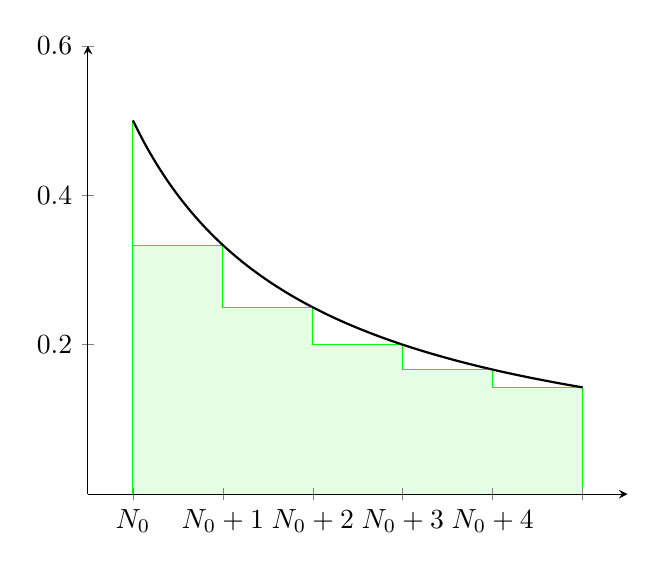
\begin{tikzpicture}[scale=1.0]
\begin{axis}[
    % xtick={0,...,1.5},ytick={0,...,1.5},
    % xmax=2,ymax=1.2,ymin=0,xmin=0,
    % enlargelimits=true,
    xticklabels={$N_0$,$N_0$,$N_0$,$N_0 + 1$,$N_0 + 2$,$N_0 + 3$,$N_0 + 4$},
    axis lines=middle,
    clip=false,
    ymax=0.6,
    ymin=0,
    xmin=1.5,
    xmax=7.5,
    domain=2:7,
    axis on top
    ]

\addplot [draw=green, fill=green!10, const plot mark right, samples=6, domain=2:7]
    {1 / x}\closedcycle;

\addplot[smooth, thick,domain=2:7,samples=40]{1 / x};

\end{axis}
\end{tikzpicture}
\caption{\label{fig:integrale_maggiora_serie}L'integrale della funzione maggiora la serie}
\end{figure}

La serie \`e la somma delle aree dei rettangoli, mentre l'integrale \`e l'area sotto la curva. Vale evidentemente che:
\[
\sum_{n \ge N_0 + 1}^{\infty} a_n \le \int_{N_0 + 1}^{\infty} f(x) \dx
\]
Quindi, se l'integrale improprio converge, converge anche la serie.

Usiamo questa propriet\`a per studiare la convergenza delle serie armoniche generalizzate, come questa:
\[
\sum_{n = 1}^{\infty} \frac{1}{n^2} \le \int_{1}^{\infty} \frac{\diff x}{x^2} < \infty
\]
Il ragionamento alla base di questi confronti \`e propriamente geometrico. 

Quindi, nel caso generale, vale questo:
\[
\sum_{n = 1}^{\infty} \frac{1}{n^p} \le \int_{1}^{\infty} \frac{\diff x}{x^p} < \infty \text{ per } p > 1
\]

Come facciamo vedere, ora, che la serie diverge per $p \le 1$? Vogliamo scrivere che la sommatoria sia maggiore o uguale all'integrale, quindi dobbiamo costruire il grafico (e di conseguenza la funzione) in modo che i rettangoli della serie contengano il grafico della funzione.

\begin{figure}
\centering
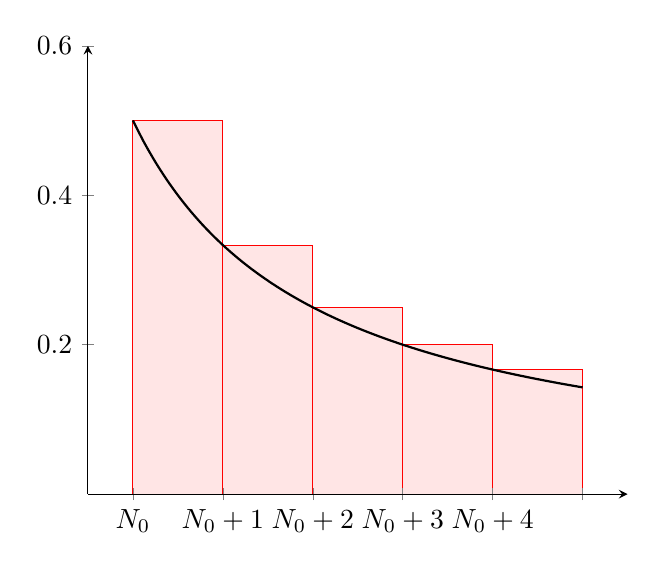
\begin{tikzpicture}[scale=1.0]
\begin{axis}[
    % xtick={0,...,1.5},ytick={0,...,1.5},
    % xmax=2,ymax=1.2,ymin=0,xmin=0,
    % enlargelimits=true,
    xticklabels={$N_0$,$N_0$,$N_0$,$N_0 + 1$,$N_0 + 2$,$N_0 + 3$,$N_0 + 4$},
    axis lines=middle,
    clip=false,
    ymax=0.6,
    ymin=0,
    xmin=1.5,
    xmax=7.5,
    domain=2:7,
    axis on top
    ]

\addplot [draw=red, fill=red!10, ybar interval, samples=6, domain=2:7]
    {1 / x}\closedcycle;

\addplot[smooth, thick,domain=2:7,samples=40]{1 / x};
\end{axis}
\end{tikzpicture}
\caption{\label{fig:serie_maggiora_integrale}La serie maggiora l'integrale della funzione}
\end{figure}

La disuguaglianza che ci interessa ora:
\[
\int_{N_0 + 1}^{\infty} f(x) \dx \le \sum_{n \ge N_0}^{\infty} a_n 
\]

Quindi, alla fine, il sottografico della funzione $f(x)$ (nella figura \ref{fig:serie_maggiora_integrale}) \`e compreso fra le due serie:
\[
\sum_{n \ge N_0 + 1}^{\infty} a_n \le
\int_{N_0 + 1}^{\infty} f(x) \dx \le 
\sum_{n \ge N_0}^{\infty} a_n 
\]
Cambia il punto di partenza delle serie (una parte da $N_0$, l'altra da $N_0 + 1$).

Ai fini pratici, ci interessa il fatto che vale questa disuguaglianza:
\[
\int_{N_0 + 1}^{\infty} f(x) \dx \le 
\sum_{n = N_0}^{\infty} a_n \le
\int_{N_0}^{\infty} f(x) \dx
\]

\begin{exmp}[di applicazione del criterio integrale]
Questa serie \`e impossibile da maggiorare o da minorare:
\[
\sum_{n = 2}^{\infty} \frac{1}{n \, \log (n) \, {\left[ \log \left( \log (n) \right) \right]}^{2}}
\]
Funziona per\`o il criterio integrale, che ci mostra che l'integrale converge:
\[
\int_{2}^{\infty} \frac{\diff x}{x \, \log(x) \, {\left[ \log \left( \log (x) \right) \right]}^{2}} = \increment{- \frac{1}{\log \left( \log(x) \right)}}^{\infty}_{2} = \frac{1}{\log \left( \log(2) \right)}
\]
Osservando la serie iniziale, e pensando all'integrale che le si pu\`o associare, si nota la presenza di una funzione e della sua derivata:
\[
\frac{1}{f'(x) \, {\left[ f(x) \right]}^2}
\]
Con $f(x) = \log \left( \log(x) \right)$, e quindi $f'(x) = \frac{1}{x \, log \left( x \right)}$.
\end{exmp}

\subsection{Criterio asintotico}

Il criterio asintotico permette di determinare la convergenza o divergenza di una serie studiando il comportamento al limite delle successioni loro associate.

Supponiamo di avere due successioni $a_n$ e $b_n$, e che valga questo:
\[
\lim_{n \to \infty} \frac{a_n}{b_n} = L \in \ooint{0}{\infty}
\]
Per un $n$ approriato, varr\`a che:
\[
\frac{L}{2} \le \frac{a_n}{b_n} \le \frac{3 \, L}{2}
\implies
\frac{L \, b_n}{2} \le a_n \le \frac{3 \, L \, b_n}{2}
\]
Quindi, se la serie di $b_n$ diverge, diverger\`a anche la serie di $a_n$, e se la serie di $b_n$ converge, converger\`a anche la serie di $a_n$.

\begin{exmp}
Consideriamo questa serie:
\[
\sum_{n = 1}^{\infty} \frac{1}{n^3 + 2 \, n - \sqrt{n} + 24}
\]
Non viene facile una maggiorazione o una minorazione: al denominatore c'\`e un $- \sqrt{n}$ che non \`e ben chiaro cosa fa. Per\`o, abbiamo il criterio del confronto asintotico per determinare la convergenza della serie. Facciamo quindi il limite del rapporto con $b_n = \frac{1}{n^3}$:
\[
\lim_{n \to \infty} \frac{n^3}{n^3 + 2 \, n - \sqrt{n} + 24} = 1
\]
Quindi, siccome questa serie converge:
\[
\sum_{n = 1}^{\infty} \frac{1}{n^3}
\]
converge anche la serie all'inizio.
\end{exmp}

\subsection{Criterio del rapporto}

Consideriamo una serie $\sum_{n} a_n$, tale per cui $a_n \ge 0$. Per verificare la convergenza o la divergenza della serie si pu\`o usare il criterio del rapporto:
\[
\lim_{n \to \infty} \frac{a_{n+1}}{a_n} = 
\begin{cases}
L < 1 \implies \sum_{n} a_n \text{ converge} \\
L > 1 \implies \sum_{n} a_n \text{ diverge} \\
1 \implies \text{ non si pu\`o dire nulla su } \sum_{n} a_n
\end{cases}
\]
Stiamo vedendo a cosa tende il rapporto fra il termine e il termine che lo precede.

\begin{exmp}
Consideriamo la serie:
\[
\sum_{n = 1}^{\infty} \frac{e^n}{n!}
\]
Applichiamo il criterio del rapporto:
\[
\lim_{n \to \infty} \frac{e^{n+1}}{(n+1)!} \cdot \frac{n!}{e^n} = 
\lim_{n \to \infty} \frac{e}{n+1} = 0
\]
Quindi la serie converge.
\end{exmp}

\subsection{Criterio della radice}

\[
\lim_{n \to \infty} \sqrt[n]{a_n} = 
\begin{cases}
L < 1 \implies \sum_{n} a_n \text{ converge} \\
L > 1 \implies \sum_{n} a_n \text{ diverge} \\
1 \implies \text{ non si pu\`o dire nulla su } \sum_{n} a_n
\end{cases}
\]
Stiamo facendo il limite per $n$ che tende all'infinito della radice $n$-esima dell'$n$-esimo termine della successione.

Entrambi questi criteri si vedono confrontandoli con la serie geometrica. Sono sempre applicazioni del criterio del confronto, da cui viene fuori la serie geometrica. \`E facile vederlo col criterio della radice.

Supponiamo il limite di $\sqrt[n]{a_n}$ sia maggiore di 1. Vuol dire che $\sqrt[n]{a_n} \ge 1 \iff a_n \ge 1$ da un certo punto in poi, e quindi $a_n$ non tende a 0, e quindi necessariamente diverge.

Supponiamo di essere nel caso in cui il limite sia minore di 1. Quindi per ogni $\varepsilon > 0$ tale per cui $L + \varepsilon < 1$, risulta che:
\[
\sqrt[n]{a_n} \le L + \varepsilon \le 1
\]
Questo equivale a dire, elevando entrambi i membri alla potenza $n$, che:
\[
a_n \le \left( L + \varepsilon \right)^{n}
\]
$L + \varepsilon$ \`e minore di 1, quindi la serie geometrica che gli associamo converge:
\[
\sum_{n = 1}^{\infty} \left( L + \varepsilon \right)^{n} \le \infty
\]
Ci siamo procurati una maggiorazione con una serie geometrica dal calcolo della radice $n$-esima di $a_n$.

Con il criterio del rapporto, invece, il ragionamento \`e questo:
\[
\frac{a_{n+1}}{a_n} \le L + \epsilon \iff a_{n+1} \le \left( L + \varepsilon \right) \cdot a_n
\]
Analogamente, valgono queste disuguaglianze:
\begin{align*}
a_{n+2} \le \left( L + \varepsilon \right) \cdot a_{n + 1} \le
\left( L + \varepsilon \right)^2 \cdot a_{n} \\
a_{n+3} \le \left( L + \varepsilon \right)^3 \cdot a_{n}
\end{align*}
E quindi ci esce di nuovo fuori una serie geometrica...

Come mai nessuno dei criteri vale quando il limite tende a 1? Boh.

% TODO riempire

\section{Serie a termini non tutti positivi}

Se non \`e vero che $a_n \ge 0$ per ogni $n$, quanto detto per il criterio del confronto non \`e pi\`u valido.

Tutti i ragionamenti fatti fino ad ora sono stati fatti con serie a termini non negativi. Cosa succede se i termini sono \emph{anche} negativi?

Se la serie \`e (anche) a termini negativi, studiamo la serie dei moduli:
\[
\sum_{n}^{\infty} \abs{a_n}
\]
\begin{defn}
Se la serie di $\abs{a_n}$ converge, si dice che la serie di $a_n$ converge \emph{assolutamente}.

Ossia, se la serie dei moduli converge, converge anche la serie di partenza. Non vale il viceversa.
\end{defn}

Supponiamo di avere una serie a termini $a_n$ anche negativi. Consideriamo la successione:
\[
b_n = a_n + \abs{a_n}
\]
Vale ovviamente che $b_n \ge 0$. Infatti, se $a_n < 0$, $a_n + \abs{a_n} = 0$, altrimenti $a_n + \abs{a_n} = 2 \, a_n \ge 0$.

Quindi $b_n \le 2 \, \abs{a_n}$. Se converge $\abs{a_n}$, converge anche $b_n$. Quindi, essendo $a_n = b_n - \abs{a_n}$, vuol dire che la serie $a_n$ converge.

Se il criterio del rapporto e il criterio della radice non funzionano, tipicamente significa che \`e necessario trovare una serie con cui fare un confronto.

\subsection{Criterio di Leibniz}

Introduciamo il criterio di Leibniz per somma di successioni a termini di segni alterno. 

\begin{theorem}[Criterio di Leibniz]
Se le seguenti ipotesi sono vere:
\begin{enumerate}
    \item $a_n \cdot a_{n+1} \le 0 \forall n$, ossia ogni termine ha segno opposto rispetto al successivo. Quindi la serie sar\`a qualcosa del tipo:
    \[
    \sum_{n} a_n = \sum_{n} (-1)^n \alpha_n
    \]
    Con $\alpha_n \ge 0$, e in particolare $\alpha_n = \abs{a_n}$.
    \item $\abs{a_{n+1}} \le \abs{a_n}$, ossia $\alpha_{n+1} \le \alpha_{n}$, ossia il valore assoluto dei termini non cresce.
    \item $\lim_{n \to \infty} a_n = 0$, ossia la successione associata alla serie tende a 0.
\end{enumerate}
allora la serie di $a_n$ converge.
\end{theorem}

\begin{proof}[del criterio di Leibniz]
Abbiamo una successione $a_n$ e, per ipotesi:
\begin{enumerate}
    \item $lim_{n \to \infty} a_n = 0$
    \item $a_n \cdot a_{n+1} < 0$
    \item $\abs{a_n} \ge \abs{a_{n+1}}$
\end{enumerate}
Senza perdita di generalit\`a, assumiamo valga $a_{2 \, n + 1} > 0$ e $a_{2 \, n} < 0$.

La serie $S_{2 \, n}$ dei termini pari \`e monotona crescente:
\[
S_{2 \, (n + 1)} = S_{2 \, n} + a_{2 \, n + 1} + a_{2 \, n + 2}
\]
Vale infatti che $a_{2 \, n + 1} > 0$ e che $a_{2 \, n + 2} < 0$, e che $\abs{a_{2 \, n + 1}} \ge \abs{a_{2 \, n + 2}}$, da cui segue che $a_{2 \, n + 1} + a_{2 \, n + 2} \ge 0$. Allo stesso modo, la serie $S_{2 \, n + 1}$ dei termini dispari \`e monotona decrescente.

Entrambe le serie sono limitate superiormente e inferiormente. Di base vale che $S_1 = a_1 > a_1 + a_2 = S_2$, e in generale che $S_{2 \, m + 1} > S_{2 \, m}$. Aggiungendoci che le serie sono una decrescente e una crescente, abbiamo che:
\[
S_1 > S_{2 \, m + 1} > S_{2 \, m} > S_2
\]
La serie dei termini dispari \`e monotona decrescente e limitata inferiormente, la serie dei termini pari \`e monotna crescente e limitata superiormente. Entrambe convergono.

Per concludere la dimostrazione, dimostriamo che convergono allo stesso valore. Infatti:
\[
\lim_{n \to \infty} S_{2 \, n + 1} - S_{2 \, n} = 
\lim_{n \to \infty} a_{2 \, n + 1} = 0
\]
La loro differenza tende a 0, quindi convergono entrambe allo stesso valore.
\end{proof}

Consideriamo questa serie:
\[
\sum_{n = 1}^{\infty} (-1)^n \frac{1}{n^p} \qquad \text{con } p \ge 0
\]
Per $p \ge 1$, sappiamo gi\`a che la serie dei moduli converge, e che quindi questa serie converge assolutamente. Ma, grazie al criterio di Leibniz, sappiamo che la serie converge anche per $0 < p \le 1$.

\subsection{Riordinare le serie}

Con serie a termini tutti positivi o tutti negativi, i termini possono essere riordinati senza problemi: si pu\`o ``commutare l'ordine degli addendi'', senza cambiare la convergenza o divergenza della serie, n\'e il valore a cui converge. Riemann dimostr\`o che non si pu\`o sempre fare lo stesso con serie a termini di segno differente.

Consideriamo questa serie:
\[
\sum_{n = 1}^{\infty} \frac{(-1)^n}{\sqrt{n}}
\]
Sommiamo prima i termini pari, fino a un certo termine $a_p$, tale per cui la somma fino a $p$ \`e maggiore di un certo numero, ad esempio $\frac{3}{4}$.
\[
\frac{1}{\sqrt{2}} + \frac{1}{\sqrt{4}} + \frac{1}{\sqrt{6}} + \ldots + \frac{1}{\sqrt{2 \, p}} > \frac{3}{4}
\]
Ora aggiungiamo i termini dispari, fino a quando la somma dei termini pari e dei termini dispari non diventa minore di $\frac{3}{4}$.
\[
\frac{1}{\sqrt{2}} + \frac{1}{\sqrt{4}} + \frac{1}{\sqrt{6}} + \ldots + \frac{1}{\sqrt{2 \, p}} - \frac{1}{\sqrt{3}} - \frac{1}{\sqrt{5}} - \frac{1}{\sqrt{7}} - \ldots - \frac{1}{\sqrt{2 \, p + 1}} < \frac{3}{4}
\]
Continuando a sommare i termini in questo modo, il risultato finale della serie riordinata sar\`a $\frac{3}{4}$: sommando i termini nel modo che abbiamo indicato, infatti, la serie \emph{tende a $\frac{3}{4}$}.

\subsubsection{Riordinare serie convergenti assolutamente}

Consideriamo una serie con termini a segno alterno:
\[
\sum_{n = 1}^{\infty} a_n \text{ t.c. } a_{2 \, k + 1} \ge 0 \land a_{2 \, k} \le 0 \forall k \in \naturals
\]
Se $\sum a_n$ converge assolutamente, allora devono convergere sia la serie dei termini dispari $\sum a_{2 \, k + 1}$, sia la serie dei termini pari $\sum a_{2 \, k}$.

Vale infatti questa disuguaglianza:
\[
\sum_{k = 1}^{N} a_{2 \, k - 1} \le \sum_{n = 1}^{2 \, N -1} \abs{a_n}
\]
Espandendola per $N = 2$, abbiamo:
\[
a_1 + a_3 \le \abs{a_1} + \abs{a_2} + \abs{a_3}
\]
La somma dei termini positivi \`e maggiorata dalla somma dei moduli di tutti i termini. Quindi vale questo, in generale:
\[
\sum_{k = 1}^{N} a_{2 \, k - 1} \le \sum_{n = 1}^{2 \, N -1} \abs{a_n}
\le \sum_{n = 1}^{\infty} \abs{a_n} < \infty
\]
Se la serie converge assolutamente, converge anche la serie dei termini positivi, poich\'e quest'ultima \`e maggiorata dalla serie dei moduli.

I termini di indice pari, invece, sono tutti negativi. La disuguaglianza che vale \`e questa:
\[
\sum_{k = 1}^{N} a_{2 \, k} \ge - \sum_{n = 1}^{2 \, N} \abs{a_n}
\ge - \sum_{n = 1}^{\infty} \abs{a_n} > - \infty
\]
La serie dei termini pari \`e \emph{minorata da un numero negativo}. La serie dei termini pari \`e minore o pari a 0, e quindi il suo valore \`e necessariamente compreso fra 0 e un numero negativo \emph{diverso da $- \infty$}. Quindi converge anche la serie dei termini pari.

Se vale che le serie dei termini pari e quella dei termini dispari convergono, allora converger\`a anche la serie normale:
\[
\sum_{n = 1}^{2 \, M} a_n = \sum_{k = 1}^{M} a_{2 \, k - 1} + \sum_{k = 1}^{M} a_{2 \, k}
\]
L'equazione che abbiamo ora scritto ha \emph{riordinato} i termini. Possiamo farlo perch\'e \emph{entrambe le serie convergono}. Se non convergessero, non si potrebbero riordinare i termini.

\subsubsection{Riordinare serie convergenti semplicemente}

Questo ragionamento non vale pi\`u per serie con termini di segno alterno che convergono \emph{semplicemente}, e che quindi non convergono assolutamente.

Se la serie converge semplicemente, vuol dire che vale questo:
\[
\sum_{k} a_{2 \, k + 1} = \infty \text{ e } \sum_{k} a_{2 \, k} = - \infty
\]
Perch\'e una serie converga semplicemente, le serie dei termini pari e dispari devono tendere rispettivamente all'infinito e a meno infinito (o viceversa). Se tendesse all'infinito positivo solo una delle due (o tutte e due), la serie divergerebbe. Se nessuna delle due tendesse all'infinito, la serie convergerebbe assolutamente.

Se si riordina una serie che converge semplicemente, la si pu\`o far tendere a qualsiasi valore, perch\'e, in realt\`a, si sta creando \emph{un'altra} serie.

% END BOH

\section{Serie di potenze}

Introduciamo le serie di potenze con un esempio.

\begin{exmp}
Consideriamo questa serie:
\[
\sum_{n = 1}^{\infty} \frac{(x - 5)^n}{\sqrt{n}}
\]
Ci chiediamo: per quali valori di $x$ questa serie converge assolutamente? Per quali converge semplicemente? Per quali \emph{non} converge? Possiamo vedere che per $x = 5$, la serie \`e la serie di tutti 0, che converge. Per $x = 6$, la serie diverge.

In generale, se $x \ge 5$, la serie \`e una serie a termini positivi, e quindi possiamo applicare i criteri che abbiamo gi\`a visto. Ad esempio, si pu\`o applicare il criterio del rapporto.
\[
\lim_{n \to \infty} \frac{(x - 5)^{n+1}}{\sqrt{n+1}} \, \frac{\sqrt{n}}{(x - 5)^n} = \lim_{n \to \infty} (x - 5) \frac{\sqrt{n}}{\sqrt{n+1}} = (x - 5)
\]
Quindi il rapporto tende a $x - 5$. Se $5 < x < 6$, la serie converge, quindi sappiamo che la serie converge per $x \in \coint{5}{6}$, diverge per $x \in \coint{6}{\infty}$.

Per scoprire dove converge assolutamente, studiamo la serie:
\[
\sum_{n = 1}^{\infty} \frac{\abs{x - 5}^n}{\sqrt{n}}
\]
Applicando il criterio del rapporto a questa serie troviamo che converge per $\abs{x - 5} < 1$, e che diverge per $\abs{x - 5} > 1$.

Quindi, per $\abs{x - 5} < 1$, ossia per $4 < x < 5$, la serie converge assolutamente. Per $x$ pari a $5$, la serie diverge. Per $x$ pari a $4$, la serie converge, essendo uguale a:
\[
\sum_{n = 1}^{\infty} \frac{(-1)^n}{\sqrt{n}}
\]
Che converge (semplicemente) per il criterio di Leibniz.
\end{exmp}

Per studiare queste serie, si applica il criterio del rapporto alla serie dei moduli, per trovare gli intervalli in cui la serie converge assolutamente. Poi, si studiano i punti in cui il criterio del rapporto ha limite 1, per scoprire se la serie converge o diverge anche in quei punti.

Le serie di potenze sono serie nella forma:
\[
\sum_{n = 0}^{\infty} a_n \cdot (x - x_0)^n
\]
$x_0$ \`e chiamato ``centro''. I casi che possono verificarsi sono:
\begin{enumerate}
    \item la serie converge solo per $x = x_0$
    \item la serie converge per ogni $x$
    \item esiste un numero $R \in \ooint{0}{\infty}$ tale che la serie converge assolutamente per $\abs{x - x_0} < R$ e non converge per $\abs{x - x_0} > R$. Non diciamo niente sui casi in cui $\abs{x - x_0} = R$.
\end{enumerate}

Per verificare cosa succede, facciamo subito la sostituzione $y = x - x_0$, e riconduciamoci alla serie seguente (di centro 0):
\[
\sum_{n = 0}^{\infty} a_n \cdot y^n
\]
Studiamo la serie dei moduli, cercando per quali valori di $y$ si ha che $\abs{a_n} \cdot \abs{y}^n < \infty$.

Dobbiamo applicare il criterio del rapporto, avendo una serie a termini positivi.
\[
\lim_{n \to \infty} \frac{\abs{a_{n+1}} \cdot \abs{y}^{n+1}}{\abs{a_n} \cdot \abs{y}^n} = \frac{\abs{a_{n+1}}}{\abs{a_n}} \cdot \abs{y}
\]
Supponiamo che il limite $\frac{\abs{a_{n+1}}}{\abs{a_n}}$ tenda a un certo $L \in \ooint{0}{\infty}$. Quindi il limite del rapporto tende a $\abs{y} \cdot L$.
\begin{itemize}
    \item se $\abs{y} \cdot L < 1$, la serie converge assolutamente.
    \item se $\abs{y} \cdot L > 1$, la serie diverge.
    \item se $\abs{y} \cdot L = 1$, non sappiamo niente.
\end{itemize}

La serie converge assolutamente per $\abs{y} < \frac{1}{L}$, quindi per $\abs{x - x_0} < \frac{1}{L}$, ossia:
\[
x_0 - \frac{1}{L} < x < x_0 + \frac{1}{L}
\]
$R = \frac{1}{L}$ si chiama \emph{raggio di convergenza}.

\begin{exmp}
Consideriamo questa serie di potenze:
\[
\sum_{n = 1}^{\infty} \frac{x^n}{n^p} \forall p
\]
Il centro della serie \`e 0. Il suo raggio di convergenza \`e 1:
\[
\lim_{n \to \infty} \frac{n^p}{(n+1)^p} = 1
\]
Quindi la serie converge assolutamente per $-1 < x < 1$. Ma per $x = 1$ e per $x = -1$? Dobbiamo studiare questi casi a parte.

Per $x = 1$, la convergenza e divergenza dipende dal valore del parametro $p$.
\[
\sum_{n = 1}^{\infty} \frac{1}{n^p} < \infty \iff p > 1
\]
Per $x = -1$, la serie diventa:
\[
\sum_{n = 1}^{\infty} \frac{(-1)^n}{n^p}
\]
\`E una serie a termini di segno alterno. Se $p > 1$, la serie converge assolutamente, poich\'e la serie dei moduli \`e quella appena vista. Per $0 < p \le 1$, la serie converge semplicemente.

In sintesi, la serie converge assolutamente per $\abs{x} < 1$, non converge per $\abs{x} > 1$.

Per $x = 1$, la serie converge $\iff p > 1$.

Per $x = -1$, la serie converge assolutamente se $p > 1$, converge semplicemente se $0 < p \le 1$.
\end{exmp}

\subsection{Serie di potenze, derivate, e integrali}

Consideriamo una generica serie di potenze:
\[
\sum_{n = 0}^{\infty} a_n \, (x - x_0)^n
\]
con raggio di convergenza $R \in \ocint{0}{\infty}$. Vuol dire che la serie converge per $- R < x - x_0 < R$.

Possiamo vedere questa serie come una funzione $f(x)$, definita per $\abs{x - x_0} < R$, ossia per $x \in \ooint{x_0 - R}{x_0 + R}$ (che \`e chiamato \emph{intervallo di convergenza}). 
\[
f(x) = \sum_{n = 0}^{\infty} a_n \, (x - x_0)^n
\]
Questa funzione \`e derivabile, e la sua derivata \`e la somma delle derivate:
\[
f'(x) = \sum_{n = 1}^{\infty} n \, a_{n} \, (x - x_0)^{n - 1}
\]
E non solo: essendo derivabile, questa funzione \`e anche integrabile:
\[
\int_{x_0}^{x} f(x) \dx = 
\sum_{n = 0}^{\infty} \int_{x_0}^{x} a_n \, (x - x_0)^n =
\sum_{n = 0}^{\infty} a_n \, \frac{(x - x_0)^{n + 1}}{n + 1}
\]
Le serie di potenze sono integrabili e derivabili termine a termine \emph{all'interno dell'intervallo di convergenza}. E il discorso, poi, vale anche per la derivata della derivata, e per la derivata della derivata della derivata... La derivata $k$-esima \`e:
\[
f^{(k)} (x) = \sum_{n = k} n \cdot (n - 1) \cdot \ldots \cdot (n - k + 1) \, a_n \, (x - x_0)^{n - k}
\]
Dicendo che $0^0 = 1$ (\`e un abuso di notazione, ma a noi va bene), vediamo quanto vale la funzione (e le sue derivate) in $x = x_0$:
\begin{align*}
f(x_0) &= a_0 \\
f'(x_0) &= a_1 \\
f''(x_0) &= 2 \, a_2 \\
&\vdots \\
f^{(k)}(x_0) &= k! \, a_k
\end{align*}
Abbiamo scritto poco sopra, infatti:
\[
f^{(k)} (x_0) = \sum_{n = k} n \cdot (n - 1) \cdot \ldots \cdot (n - k + 1) \, a_n \, (x_0 - x_0)^{n - k} =
k \cdot (k - 1) \cdot \ldots \cdot 1 \, a_{k} = k! \, a_{k}
\]
$0^0$ \`e un abuso di notazione perch\'e quello che si dovrebbe scrivere \`e:
\[
a_0 + \sum_{n = 1}^{\infty} a_n \, (x - x_0)^n
\]
Ma, siccome $n^0 = 1 \forall n \in \reals - \{ 0 \}$, si preferisce abusare della notazione matematica e scrivere:
\[
\sum_{n = 0}^{\infty} a_n \, (x - x_0)^n
\]
Quindi, sapendo che $a_k = \frac{f^{(k)}(x_0)}{k!}$, possiamo riscrivere:
\[
f(x) = \sum_{n = 0}^{\infty} a_n \cdot (x - x_0)^n =
\sum_{n = 0}^{\infty} \frac{f^{(n)} (x_0)}{n!} \cdot (x - x_0)^{n}
\]
Che \`e la famosa serie di Taylor.

Ogni serie di potenze \`e, all'interno dell'intervallo di convergenza, la serie di Taylor della sua somma.

A cosa ci serve questo? Sappiamo una cosa:
\[
\sum_{n = 0}^{\infty} x^n = \frac{1}{1 - x}
\]
Quindi, $f(x)$ vale:
\[
f(x) = \frac{1}{1 - x}
\]
Quale \`e la derivata $k$-esima di questa funzione nell'origine? L'abbiamo visto prima: $a_n$ \`e sempre 1, e quindi:
\[
f^{(k)} (0) = k!
\]
Guardiamo questa funzione:
\[
f(x) = \frac{1}{(1 - x)^2}
\]
\`E il quadrato \emph{e} la derivata di $\frac{1}{1 - x}$. Quale \`e il suo sviluppo in serie?
\[
\frac{1}{(1 - x)^2} = \left[ \frac{1}{1 - x} \right]' = 
\sum_{n = 0}^{\infty} \left[ x^{n} \right]' = \sum_{n = 1}^{\infty} n \, x^{n - 1}
\]
La derivata della funzione (che \`e la serie), \`e la serie delle derivate! Il termine con $n = 0$ scompare, una volta derivato: \`e una costante.

Prendiamo quest'altra funzione:
\[
\frac{1}{1 + x} = \sum_{n = 0}^{\infty} (-1)^n \, x^n
\]
Si vede chiaramente, infatti \`e sufficiente sostituire $x$ con $-x$ nell'equazione di poco sopra...

Quale sar\`a lo sviluppo in serie di potenze di questa funzione?
\[
f(x) = \log (1 + x)
\]
\`E una primitiva della funzione vista sopra... Quindi il suo sviluppo in serie di potenze sar\`a:
\[
\log (1 + x) = \sum_{n = 0}^{\infty} (-1)^n \, \frac{x^{n+1}}{n+1}
\]
Sviluppandolo viene questo:
\[
\log (1 + x) = x - \frac{x^2}{2} + \frac{x^3}{3} - \frac{x^4}{4} + \ldots
\]
Tutto questo vale all'interno dell'intervallo di convergenza. Quest'ultimo caso sarebbe vero anche per $x = 1$, anche se l'intervallo di convergenza \`e $-1 < x < 1$. Sostituendo $x = 1$ troviamo questo:
\[
\log (2) = \sum_{n = 1}^{\infty} \frac{(-1)^{n+1}}{n}
\]
La serie armonica a termini di segno alterno vale $\log (2)$.

Sappiamo quanto vale questa serie:
\[
\sum_{n = 0}^{\infty} (-1)^n x^{2 \, n} = \frac{1}{1 + x^2}
\]
La primitiva di una somma \`e la somma delle primitive... E la primitiva di una serie \`e la serie delle primitive.
\[
\arctan (x) = \sum_{n = 0}^{\infty} (-1)^n \frac{x^{2 \, n + 1}}{2 \, n + 1}
\]
Anche qui si pu\`o fare qualche operazione impropria: per $x = 1$, abbiamo uno sviluppo in serie di $\arctan (1) = \frac{\pi}{4}$.

Quando scriviamo un polinomio di Taylor come questo:
\[
f(x) = \sum_{n = 0}^{N} \frac{f^{(n)} (x_0)}{n!} \, (x - x_0)^n
\]
Stiamo trascurando un errore, dipendente da $N$:
\[
E_N (x) = \frac{f^{(N + 1)} (\xi)}{(N + 1)!} \, (x - x_0)^{N + 1}
\]
La serie di Taylor \`e il limite del polinomio di Taylor, per $N \to \infty$.

Studiamo questa serie:
\[
\sum_{n = 0}^{\infty} \frac{x^n}{n!}
\]
Il raggio di convergenza \`e $\infty$, quindi converge per ogni $x$. Questo polinomio qui:
\[
\sum_{n = 0}^{N} \frac{x^n}{n!} + E_N (x)
\]
\`e il polinomio di Taylor di $e^x$ di centro uguale a 0. Le derivate di $e^x$ sono tutte $e^x$, e nell'origine valgono sempre 1. L'errore varr\`a:
\[
E_N (x) = e^\xi \cdot \frac{x^{N+1}}{(N+1)!}
\]
Maggioriamo l'errore cos\`i:
\[
\abs{E_N (x)} \le \frac{e^{\abs{x}} \, \abs{x}^{N+1}}{(N + 1)!}
\]
Per $N$ che tende all'infinito, l'errore tende a 0. Quindi la serie di prima \`e la serie di Taylor di $e^x$:
\[
e^x = \sum_{n = 0}^{\infty} \frac{x^n}{n!}
\]
Ripeschiamo il polinomio di Taylor della funzione seno:
\[
\sin (x) = x - \frac{x^3}{3!} + \frac{x^5}{5!} - \frac{x^7}{7!} + \ldots
\]
La serie di Taylor della funzione sar\`a il limite per $n \to \infty$ del polinomio di Taylor.






























\clearpage

\chapter{Roba utile}

\section{Integrali immediati utili}

\begin{gather*}
\int x^{\alpha} \dx = 
\begin{cases}
\frac{x^{\alpha + 1}}{\alpha + 1} + c \text{ se } \alpha \neq -1 \\
\abslog{x} + c \text{ se } \alpha = -1
\end{cases} \\
\int f(\alpha \, x) \dx = \frac{F(\alpha \, x)}{\alpha} + c \\
\int \sin (x) \dx = - \cos (x) + c \\
\int \cos (x) \dx = \sin (x) + c \\
\int \frac{\diff x}{\cos^2 (x)} = \int \sec^2 (x) \dx = \tan (x) + c \\
\int \frac{\diff x}{\sin^2 (x)} = \int \csc^2 (x) \dx = \cot (x) + c \\
\int \tan (x) \dx = - \abslog{\cos (x)} + c \\
\int \cot (x) \dx = \abslog{\sin (x)} + c \\
\int \sec (x) \, \tan (x) \dx = \int \frac{\sin(x)}{\cos^2 (x)} \dx =
- \frac{1}{\cos(x)} + c \\
\int \frac{1}{\sqrt{a^2 - b^2 \, x^2}} \dx =
\frac{1}{a} \, \arcsin \left( \frac{a}{b} \, x \right) + c
\end{gather*}

\section{Equivalenze trigonometriche}

Equivalenze fra funzioni trigonometriche:
\begin{align*}
\tan (x) &= \frac{\sin(x)}{\cos(x)} & \sec (x) &= \frac{1}{\cos(x)}  \\
\cot (x) &= \frac{\cos(x)}{\sin(x)} & \csc (x) &= \frac{1}{\sin(x)}
\end{align*}

L'equivalenza pi\`u semplice \`e:
\[
\cos^2 (x) + \sin^2 (x) = 1
\]

\subsection{Duplicazione}

Le formule di ``duplicazione'' che si vedono generalmente:
\begin{align*}
\cos(\alpha + \beta) &= \cos(\alpha) \, \cos(\beta) - \sin(\alpha) \, \sin(\beta) \\
\cos(\alpha - \beta) &= \cos(\alpha) \, \cos(\beta) + \sin(\alpha) \, \sin(\beta) \\
\sin(\alpha + \beta) &= \sin(\alpha) \, \cos(\beta) + \cos(\alpha) \, \sin(\beta)\\
\sin(\alpha - \beta) &= \sin(\alpha) \, \cos(\beta) - \cos(\alpha) \, \sin(\beta)
\end{align*}
% Sono facili da memorizzare: \emph{coscia coscia, seno seno} e \emph{seno coscia, coscia seno}.

Da queste si ricavano due formule di vera duplicazione:
\begin{align*}
\sin( 2 \, x) &= 2 \, \sin (x) \, \cos (x) \\
\cos (2 \, x) &= \cos^2 (x) - \sin^2 (x)
\end{align*}
E dall'ultima in particolare, si tira fuori un'equivalenza per il $\sin^2$ e il $\cos^2$:
\begin{align*}
\cos^2 (x) &= \frac{1 + \cos (2 \, x)}{2} \\
\sin^2 (x) &= \frac{1 - \cos (2 \, x)}{2}
\end{align*}

Un'ultima formula di duplicazione, generale ma poco utile:
\[
\sin(\alpha) - \sin(\beta) = 
2 \, \sin \left( \frac{\alpha - \beta}{2} \right) \, \cos \left( \frac{\alpha + \beta}{2} \right)
\]

\subsection{Limiti notevoli}

Le funzioni trigonometriche hanno qualche limite notevole associato. Il primo che si vede \`e:
\[
\lim_{x \to 0} \frac{\sin (x)}{x} = 1
\]
Sostituendo $x$ con $\frac{1}{y}$ (e mandando il limite all'infinito) si pu\`o scrivere come:
\[
\lim_{y \to \infty} \frac{\sin \left( \frac{1}{y} \right) }{\frac{1}{y}} = 1
\]
Vale ovviamente un limite simile con la tangente:
\[
\lim_{x \to 0} \frac{\tan (x)}{x} = 1
\]

Poi c'\`e il limite notevole del coseno:
\[
\lim_{x \to 0} \frac{1 - \cos (x)}{x^2} = \frac{1}{2}
\]
Attenzione all'$x^2$! Con $x$ vale infatti questo:
\[
\lim_{x \to 0} \frac{1 - \cos (x)}{x} = 0
\]


\clearpage

\end{document}
